\documentclass[A4paper, 11pt]{book}
\usepackage{Informatica}
\usepackage{listings}


\title{\Huge \bfseries \scshape Informatica 1}
\author{\Large \bfseries \scshape Lorenzo Uboldi}
%\title{}
%\author{}
\date{}
%\titlepic{\includegraphics[width=\textwidth]{copertina.png}}
\makeindex

\begin{document}

	\frontmatter
	\maketitle
	
	% Colophon
	\null % Bisogna inserire qualcosa prima di \vfill, altrimenti non funziona
	\vfill % Riempie lo spazio verticale della pagina
	\hspace*{-1.5em}\includegraphics[scale=.7]{Immagini/by-nc-sa-eu.eps}
	\begin{flushleft}
		Quest'opera è stata rilasciata con licenza \emph{Creative Commons} Attribuzione - Non commerciale - Condividi allo stesso modo 4.0 Internazionale. Per leggere una copia della licenza visita il sito web \url{http://creativecommons.org/licenses/by-nc-sa/4.0/}.\\[1cm]
		Versione aggiornata al \today,\\
		Lorenzo Uboldi (\href{mailto:lorenzo.uboldi@studenti.unimi.it}{\ttfamily lorenzo.uboldi@studenti.unimi.it}), Milano.\\[0.2cm]
		L'ultima versione, aggiornata e rivista, è sempre disponibile a: \url{https://github.com/ulorentz/Informatica1}
	
	\end{flushleft}

	\cleardoublepage
	\pdfbookmark[1]{Indice}{tableofcontents}
	\tableofcontents %metto all'inizio l'indice
	
	%Prefazione, dopo l'indice o prima?
	\chapter{Guida alla lettura}
Questo scritto  è ``a più livelli''. Come noterai sono presenti diverse note a piè di pagina, appendici, ecc\ldots Tutto ciò è un ``di più'', non strettamente necessario a passare l'esame, ma se da subito ti accorgi che l'Informatica ha un suo fascino, potrebbe stimolarti ad ``andare oltre'': qualche piccola curiosità quà e là, qualche approfondimento, qualche chiarimento\ldots

Ovviamente, puoi saltare tutto e andare solo al dunque. 

In appendice, sono presenti una rapida guida per familiarizzare con Linux, una guida per l'installazione di ROOT e qualche tema d'esame risolto.\\


Ci tengo a sottolineare una cosa: queste note non sono appunti del corso o, tanto meno, una ``\emph{dispensa del corso}'' ufficiale. Piuttosto, dopo essermi appassionato all'Informatica e dopo aver approfondito questa materia, ho deciso, anni dopo il corso, di provare a ``buttare giù'' qualche riga. Ti dico tutto ciò per metterti in guardia: ho seguito una mia linea espositiva cercando di coprire tutti gli argomenti del corso, ma lungi da me l'intento di sostituirmi alle lezioni, preziosissime e da frequentare! Confrontati sempre con loro!\\

Infine, così come il corso, queste note sono pensate per essere ``introduttive'' al \verb|C++| e alla programmazione; per cui, a volte, l'esposizione è semplicistica per favorire la comprensione. Sappi, però, che il \verb|C++| è estremamente più vasto, complesso e completo di quanto da queste note possa apparire, citando l'autore del libro che più mi ha istruito\footnote{Thinking in C++, Bruce Eckel}: ``\emph{C} -e, per eredità, il \verb|C++|- \emph{ has never been a language to bar entry where others fear to tread}''. \\

Detto ciò, buona lettura\ldots Ah, se trovi imprecisioni, errori o chissà quale altra castroneria, segnalamela (\href{mailto:lorenzo.uboldi@studenti.unimi.it}{\ttfamily lorenzo.uboldi@studenti.unimi.it}), te ne sarò grato!
	\chapter{Leggimi please!}
L'attuale versione di queste note è un \emph{work in progress}: in primis non è ancora completa, in secondo luogo è in corso di revisione. Purtroppo, vi sarà sicuramente qualche errore. 

Essendo uno dei primi lettori, ti chiedo gentilmente di comunicarmi tutto per poter correggere (\href{mailto:lorenzo.uboldi@studenti.unimi.it}{\ttfamily lorenzo.uboldi@studenti.unimi.it}), grazie!

(Mi auguro di far sparire al più presto questa stupida pagina\ldots)
	\mainmatter
	%Capitoli
	\chapter{Introduzione alla programmazione}
Tutti i giorni, quando accendiamo il computer o usiamo il nostro smartphone, abbiamo a che fare con programmi. Ti sei mai chiesto cosa c'è sotto? Come è nato e come è stato costruito quel programma?

Se anche queste domande non ti avessero mai neanche lontanamente sfiorato, nel corso di Informatica 1 ti toccherà imparare le basi del retroscena dei programmi che usi con nonchalance tutti i giorni. Vedremo giusto le fondamenta della programmazione, niente di più! Chi lo sa, magari troverai perfino interessante questo mondo\ldots

Bando alle ciance, iniziamo!
\section{Com'è fatto un computer?}
Il computer (calcolatore in inglese) è una macchina in grado di eseguire istruzioni e di fare calcoli:  per come lo schematizzeremo noi, è composto dal processore, dalla memoria RAM e dai dispositivi di input e output. 

Il processore è la parte che fa i conti, che ragiona: è il cervello del computer, è la parte pensante.

La memoria di cui parleremo, trattando di programmazione, è sempre la RAM (Random Access Memory); quando un programma ``gira'', viene caricato sulla RAM, non sull'hard disk. Sistema operativo, drivers, programmi ``vivono'' tutti nella RAM: questa è la memoria con cui ci interfacciamo quando programmiamo. 

I dispositivi di input sono (al nostro livello) solo due: la tastiera e l'hard disk. I files, infatti, a differenza dei programmi, sono archiviati sull'hard disk e un programma può accedervi facilmente, sia in lettura che in scrittura. L'hard disk è, quindi, sia un dispositivo di output che di input.
\\L'altro dispositivo di output sarà, per noi, lo schermo.

\section{Cosa vuol dire programmare?}
Il computer è una macchina che ragiona in linguaggio binario: la lingua che ``parla'' è fatta di 0 e 1. Ovviamente i computer non nascono ``imparati'', loro sanno fare solo conti: bisogna istruirli su che conti fare. 

Un programma non è altro che un'istruzione per il computer, un'insieme di parole (del computer, non le nostre parole!) che, una dopo l'altra, con la loro logica, rappresentano dei calcoli e delle operazioni.
\subsection{Linguaggio macchina}
Ecco quindi introdotto il concetto di linguaggio macchina: è una serie di 0 e 1 che rappresentano istruzioni. Il computer, oltre a saper elaborare questi 0 o 1, li sa immagazzinare: l'unità logica che può contenere questo dato è il \emph{bit} (un bit o vale zero o vale uno). La memoria del computer è, in realtà, organizzata in \emph{byte}: un byte è composto da 8 bit. Il byte è l'unità elementare della memoria, nei termini che interessano a noi: i dati che noi trattiamo sono sempre multipli di questa unità.

Ma torniamo al linguaggio macchina.  Se volessimo scrivere un programma (anche il più semplice, un banale calcolo) sarebbe quasi impossibile, o comunque di una complicazione estrema. 

Con la nascita dell'informatica, per rendere più agevole la scrittura di programmi da parte degli informatici, sono stati sviluppati i primi linguaggi di programmazione, decisamente più comprensibili rispetto ad una serie di 0 e 1.

\subsection{Linguaggi di programmazione}
I linguaggi di programmazione si dividono in due grandi categorie: di basso livello e di alto livello. Cosa vuol dire? Non ci si riferisce certo alla qualità, bensì a quanto il linguaggio di programmazione è vicino al linguaggio macchina. 

Un linguaggio di basso livello è composto da istruzioni elementari, del tipo: prendi il dato, spostalo in tale cella di memoria, prendi l'altro dato, spostalo nell'altra cella, ecc\ldots. 

Un linguaggio di basso livello è estremamente complicato da comprendere, e scrivere programmi complessi richiede capacità veramente notevoli, oltre a tempi ingenti. Un esempio di linguaggio di basso livello è l'\emph{assembly}.\\

I linguaggi ad alto livello sono nati per semplificare ulteriormente la vita ai programmatori: sebbene l'assembly sia molto più comprensibile dei fatidici 0 e 1, scrivere un programma in assembly è estremamente complesso e lungo. Nei linguaggi ad alto livello, molte delle istruzioni necessarie in assembly sono rese implicite. \`E tutto molto più ``chiaro'': spesso, leggendoli, sembrano una serie di istruzioni in simil-inglese. Potremmo dire che, nei linguaggi ad alto livello, al programmatore è affidata la parte logica del programma, ma non la gestione della macchina (computer), che è invece resa implicita. Linguaggi ad alto livello sono \verb|C|, \verb|C++|, \verb|Java|, \verb|Python| e molti altri.

I linguaggi ad alto livello si dividono in ``procedurali'' ed in ``orientati agli oggetti''. In realtà non credo sia fondamentale, per questo corso, capire la differenza. Ti basta sapere che \verb|C| è un linguaggio procedurale, mentre \verb|C++| (che è la sua evoluzione) è un linguaggio orientato agli oggetti. Noi studieremo quest'ultimo ma, sfortunatamente, per come viene affrontato nel corso di Informatica 1, ci limiteremo alla parte procedurale: impareremo poco di più di quanto si potrebbe studiando \verb|C|. Solo nei corsi futuri (o nelle lezioni facoltative di questo corso) affronterai la programmazione ad oggetti.

\subsection{Da C++ a linguaggio macchina}
Ma come avviene il passaggio da \verb|C++| (d'ora in poi parleremo solo di lui, non degli altri linguaggi), che come ho accennato ha elementi  di inglese e tra poco ne vedrai un esempio, a linguaggio macchina? 

Essenzialmente bisogna invocare un programma, detto compilatore, che si occupa di tradurre il \verb|C++| in linguaggio comprensibile alla CPU. Nella sezione \ref{catena} approfondiremo meglio il discorso. Per ora ti basta sapere che il compilatore esiste e fa il lavoro sporco per noi.
%Ci sono vari passaggi ma, essenzialmente, il concetto è che esiste un programma, chiamato \emph{compilatore}, che si occupa di ``tradurre'' il tuo codice in linguaggio assembly (ricordi? il linguaggio di basso livello); quindi entra in gioco l'\emph{assembler}, un programma che traduce il codice assebly in linguaggio macchina, il cosiddetto eseguibile (comprensibile dal computer). Quest'ultimo non è altro che il programma vero e proprio, che puoi lanciare ed usare.
\\

%TODO: Elimino?
%In realtà l'operazione di compilazione avviene in due passi: non lavora subito il compilatore, infatti, il primo step viene portato avanti dal \emph{preprocessore}. Il preprocessore si occupa di preparare il file da mandare in pasto al compilatore. Sostituisce parole con intere righe di codice; se il codice si sviluppa su file differenti, prende i vari pezzi e li incolla fisicamente tutti assieme nello stesso file. Ti sembrerà di star parlando di aria fritta, ma ti dò queste informazioni perché più avanti avremo a che fare proprio con preprocessore e compilatore. In tutti i tuoi esperimenti di programmazione, ti confronterai con il compilatore, imparerai prima ad odiarlo e poi ad apprezzarlo: non si limita a tradurre il linguaggio ma ti corregge, ti dice dove e cosa hai sbagliato, e ti dà consigli. Questo vuol dire che il compilatore sa le regole del \verb|C++|, si accorge di errori all'interno del tuo codice. Il preprocessore (che incontreremo un paio di volte più avanti), invece, no: agisce sotto i tuoi piedi (non ti accorgi che sta lavorando) e non controlla moltissime cose come invece il compilatore sa fare. Il preprocessore, quindi, non ti avvisa di molti errori che potresti commettere nel codice che lo riguarda. Vedremo che, mentre in una situazione il preprocessore è fondamentale, nelle altre lo si può evitare.\\

	
Ma basta parlar di teoria, è arrivato il momento di vedere un po' di codice!
\section{Il tuo primo programma}
Ti riporto un esempio di programma e poi (promesso!) ti spiegherò tutto: cosa vogliono dire quelle strane parole, ma anche come compilare tutto ciò ed eseguirlo!

\subsection{Il codice}
\begin{lstlisting}
#include<iostream>
using namespace std;

int main(){//Qui inizia il nostro programma
	cout << "Hello World!" << endl;
	return 0; //e qui finisce
}
\end{lstlisting}
Analizziamo riga per riga: 
\begin{itemize}


\item\textbf{\#include<iostream>} Questa è una direttiva per il preprocessore (così come lo è tutto ciò che inizia con \#). Stiamo dicendo al preprocessore di includere nel nostro codice l'\emph{header} (dall'inglese: intestazione) di una libreria, \emph{iostream}. L'\emph{header}  è essenzialmente un file dentro cui è contenuto del codice dove sono dichiarati degli ``strumenti''; includendolo nel nostro codice possiamo usare gli strumenti della libreria\footnote{Nel capitolo \ref{lib}, vedremo  che per usare le librerie scritte da noi dovremo fare qualche passo in più.}.

Includere l'\emph{header} di una libreria vuol dire che il preprocessore va a cercare il file dove è contenuto, copia tutto il codice e lo incolla al posto della riga ``\#include \ldots'': ci risparmia un noiosissimo lavoro e ci evita di lavorare con file composti da migliaia di righe di codice, magari neanche scritte da noi. 

Per le librerie standard del \verb|C++|, includere l'\emph{header} è tutto ciò che dobbiamo fare per poter usare la libreria per cui, d'ora in poi, con un abuso di linguaggio, dirò ``includere la libreria'' per rendere più chiaro il concetto.

Iostream vuol dire ``in-out stream'', ovvero canale di ingresso e uscita. Lì dentro sono definite alcune funzioni per comunicare con l'utente, come quelle per stampare a video parole e numeri o quelle per leggere da tastiera degli input. 

Anche se ancora non abbiamo parlato di in e out, includi sempre nei tuoi programmi \emph{iostream}.

\item\textbf{using namespace std;} Te lo dico subito: questo codice ti rimarrà oscuro fino alla fine del corso. Spiegarti cosa significa vorrebbe dire immergersi in un argomento, il \emph{namespace}, che non userai mai in questo corso. Quindi evitiamo. Solo una cosa: ricordati di metterlo in ogni file dopo le inclusioni delle librerie. È importante!


\item\textbf{int main()\{ \}} Eccoci qua: questo è il programma vero e proprio! Main() è una funzione (nei prossimi capitoli impareremo di più sulle funzioni), è l'``entità'' che viene lanciata dal sistema operativo (d'altronde, ``main'', significa ``principale''), è qui che inizia il programma vero e proprio!

Il programma è tutto ciò che è racchiuso tra le due parentesi graffe, può essere scritto su file differenti, può svilupparsi in migliaia di righe di codice ma, sul piano logico, tutto è racchiuso tra queste due parentesi. 

In poche parole, in ogni programma che scrivi deve esistere il \emph{main}: tutto si svolge tra quelle parentesi graffe. Senza \emph{main} non esiste il programma (e se per caso provi a compilare un file sorgente senza \emph{main}, il compilatore ti avvisa della sua mancanza e non compila).

\item\textbf{//} Il doppio slash è il simbolo in \verb|C++| per inserire un commento. Cos'è un commento? \`E qualcosa che viene completamente ignorato dal compilatore, può quindi essere inserito nel codice per commentare quello che abbiamo scritto senza intaccare la funzionalità del programma. Ad esempio, può trattarsi di frasi per spiegare i vari passaggi del nostro codice ed aumentarne la comprensibilità. 

I commenti in \verb|C++| sono tutto ciò che segue il doppio slash (rimanendo sulla stessa riga). Oppure tutto ciò che è contenuto tra ``/*'' e ``*/'': il primo simbolo dà inizio al commento, il secondo lo conclude; possono essere anche molte righe e non semplicemente una!

\item\textbf{cout\ldots endl;} Cout è l'abbreviazione di ``console output'': è il codice per utilizzare il dispositivo di output primario, lo schermo (tramite il terminale, che tra poco introdurremo). Quando vogliamo stampare a video qualcosa, dobbiamo chiamare la funzione \emph{cout}. Questa parola va seguita da ``\verb|<<|'' che,	 simbolicamente, rappresenta un flusso in uscita. Dopo possiamo mettere ciò che vogliamo stampare: una stringa di lettere racchiusa tra virgolette, come il nostro ``Hello World!'', o una variabile (vedi il prossimo capitolo). 

Alla fine dobbiamo ``mandare a capo'',  e per farlo inseriamo di nuovo il simbolo ``<<'' seguito dalla parola \emph{endl}, che significa ``end line'': appunto, ``vai a capo!''.
	
\item\textbf{return 0;} In tutte le chiacchiere che andremo a fare non ci occuperemo mai di sistemi operativi, di cosa fanno, di perché esistono e a cosa servono (puoi, però, trovare una brevissima introduzione all'uso di Linux in appendice \ref{linux}). 

In ogni caso, in questa riga stiamo comunicando con il sistema operativo. Essenzialmente quando il programma arriva a questo punto si conclude. Nel finire, però, restituisce qualcosa al sistema operativo (un numero): ``0'' sta per ``va tutto bene''. Se tutto non va bene, puoi restituire al sistema operativo un altro numero, ma è una finezza\ldots

\item\textbf{Il punto e virgola!}
Puoi vedere il codice di un programma \verb|C++| come una serie di istruzioni e operazioni. Ogni istruzione va conclusa, bisogna dire al compilatore: ``l'istruzione finisce qua, quello che segue è un'altra cosa!''. Mandare a capo non ha questo significato (mandare a capo rende più leggibile il codice per il programmatore, e se tu non mandassi a capo compilerebbe lo stesso, ma per carità, non lo fare!): è il punto e virgola che conclude un'istruzione! Alla fine di ogni unità logica è necessario un punto e virgola. 

Ci sono solo due situazioni del codice dove non ci vuole il punto e virgola, anche se viene conclusa un'unità logica: alla fine di una direttiva per il preprocessore e dopo la chiusura di una parentesi graffa (esistono delle eccezioni a quest'ultimo caso, le vedremo più avanti).

Nel mio codice, come puoi vedere, dopo ``\verb|#include <iostream>|'' non c'è un punto e virgola. Non c'è nemmeno dopo la chiusura della graffa del \emph{main}.
\end{itemize}
Tutto chiaro?
\subsection{Spazio di tab e leggibilità del codice}
Mandare a capo non è l'unica cosa che rende il codice più leggibile: ce n'è una seconda che, purtroppo, all'inizio gli studenti sono davvero restii a fare, ma è importante!


Ciò che è racchiuso tra due parentesi graffe è detto \emph{scope} (vedi il prossimo capitolo per una definizione migliore): ogni volta che apriamo una parentesi graffa stiamo scrivendo un piccolo ``capitolo'' del nostro codice (e alla fine di questo capitolo la parentesi va chiusa). \`E elegante, e rende il codice molto più agevole da leggere, dare uno spazio di tab in più (tasto della tastiera)  per gli elementi all'interno delle graffe, uno spazio in più rispetto al ``livello'' delle graffe. 

Ti faccio un esempio di codice, ma non cercare di capire ciò che succede, semplicemente mi interessa che ti chiarisca le questioni grafiche.
	
	\begin{lstlisting}
#include <iostream>
using namespace std;
int main(){ //apro graffa, tutto cio' che segue va preceduto da uno spazio di tab
	int j=10;
	for(int i=0; i<10; i++){//nuovo scope, ci vuole un ulteriore spazio di tab
		cout << i << endl;
		if(i==5){//nuovo scope, nuovo spazio!
			cout << "Sono a meta'!" << endl;
		} //chiudo al ``livello'' dell'apertura
	} 
	return 0;
}
	\end{lstlisting} 
Questa tecnica aiuta a capire cosa è dentro cosa, con una sorta di matriosca di graffe. Aiuta a distinguere graficamente i vari ``capitoli'' del nostro codice. Dà un impatto grafico agli scopes\footnote{In alcuni linguaggi, come il Python, non esistono le parentesi graffe che delimitano gli scopes, ma sono proprio gli spazi di tab a definirli. Prendere l'abitudine ad usare gli spazi di tab ti faciliterà la vita se vorrai imparare un linguaggio di quel tipo (e a Fisica, in alcuni corsi, il Python ti sarà richiesto).}. 

Ti assicuro che rende il tuo codice molto più leggibile, per te e per gli altri. Inoltre, mancare di questa accortezza ti fa togliere punti all'esame.
\\

La leggibilità del codice non è da sottovalutare, e un'altra cosa che aiuta a renderlo più leggibile sono i commenti. Commentare tanto (spiegando quello che fai) rende tutto più chiaro, non solo a chi deve leggere quello che hai scritto, ma anche a te stesso! Se dopo mesi riprendi in mano un tuo programma e lo devi modificare, ti posso assicurare che non ti ricorderai niente di quello che hai scritto: avere tanti bei commenti ti risparmierà ore a cercare di capire cosa ti era passato per la testa mesi prima. Se poi stai scrivendo codice con altri, commentare è davvero importantissimo: non tutti sono nella tua testa! (Neanche il prof all'esame\ldots)

\section{Il file sorgente, il terminal e il compilatore}
Ho parlato di codice e te ne ho introdotto uno molto semplice, ma credo che ancora non ti sia chiaro dove va fisicamente scritto, come va compilato e, una volta fatto ciò, come si usa il programma.

\subsection{Quale sistema operativo?}
Ho promesso che non mi sarei dilungato a parlare di sistemi operativi, ma un piccolo accenno, puramente pratico, conviene farlo. 

L'ambiente di programmazione ideale è il sistema operativo Linux. Linux è completamente free (open source) ed è altamente performante, tanto che si adatta perfettamente ai centri di calcolo, server di Google, supercomputer, ecc\ldots 

Se non disponi di Linux, te lo puoi procurare installandolo su un tuo computer, in una partizione dedicata o in virtual machine. Consiglio, tra le tante distribuzioni, Ubuntu o una sua derivata (Kubuntu o, se hai un computer non molto prestante, le più leggere Xubuntu o Lubuntu): in università molti hanno questa distribuzione e puoi trovare colleghi disposti ad aiutarti, sia nell'istallazione che nell'uso. Ubuntu è user-friendly, comodo e bello da usare, ma ovviamente non è l'unica distro possibile: ce ne sono tante (altre molto valide: Fedora, Manjaro, \ldots), scegli tu quella che più ti aggrada!

Non sei obbligato ad installarti Linux, puoi lavorare usando le macchine del laboratorio in remoto anche da Windows (ovviamente con una lentezza esasperante): se sei interessato consulta la sezione ``materiale didattico'' del sito del laboratorio, dove è spiegato tutto: \url{http://www.l30-informatica.di.unimi.it/}. 

Se sei un Mac user, tienti stretto il tuo computer: va benissimo per programmare, sempre su quel sito ci sono istruzioni su come puoi fare.\\

Io uso Linux e in queste note mi baserò, nei rarissimi casi dove è necessario differenziare, su questo sistema operativo. La programmazione in \verb|C++| è uguale (al nostro livello) dappertutto: a seconda del sistema operativo cambia solo il programma con cui scrivere, come compilare e come far girare il programma stesso. 

Nell'appendice \ref{linux} ho raccolto qualche nota sull'uso di Linux, i comandi base che ti servono per lavorare a casa o in remoto, collegato al laboratorio dell'università.
\subsection{I file sorgente}
Dove si scrive il codice? Sono dei semplici file, molto simili a dei file di testo. I file di codice \verb|C++|, però, hanno un'estensione riservata: ``.cpp'' (sono estensioni del \verb|C++| anche ``.cxx'' e ``.C'', scegli tu quale preferisci\ldots). Per modificare il file sorgente hai bisogno di un editor di testo qualsiasi. I più user friendly su Linux sono Gedit e Kate. 

Apri l'editor e salva il file con l'estensione richiesta, ad esempio ``helloworld.cpp''; ora puoi scrivere il tuo codice! 

Se hai installato Lubuntu, l'editor di testo è il più sfortunato Leafpad. Non è un gran che e ti consiglio di rimuoverlo e installare Gedit. 
\\Per farlo apri il terminale (ctrl+alt+T, oppure cercalo tra i programmi) e scrivi:
	\begin{shaded}
		\begin{minipage}{\textwidth}
			\begin{verbatim}
sudo apt-get remove leafpad
			\end{verbatim}%
		\end{minipage}
	\end{shaded}
	Ti verrà chiesta la tua password e poi di confermare. 
	
	Una volta completata la disinstallazione, installa Gedit e, sempre nel terminale, scrivi:
	
	\begin{shaded}
		\begin{minipage}{\textwidth}
			\begin{verbatim}
sudo apt-get install gedit
			\end{verbatim}%
		\end{minipage}
	\end{shaded}
Conferma tutto e installa. Bene, ora sei pronto!
\\

Una volta scritto il tuo file sorgente e salvatolo con l'estensione giusta (prima salvalo, poi scrivi: così facendo Gedit capisce che è codice \verb|C++| e ti colora le parole del linguaggio), è arrivato il momento di compilare!

Due parole per i Mac users: usate Xcode. Lì scrivete il vostro codice e salvate (sempre con estensione ``.cpp''); non usate Xcode per compilare, ma il terminal: questo è per essere in un ambiente più simile a quello che userete all'esame!

\subsection{Il terminale e il compilatore}
Abbiamo detto che, una volta scritto il codice sorgente, bisogna compilarlo; il programma che effettua questa operazione è il compilatore. Per lanciare quest'ultimo abbiamo bisogno del terminal. Il terminale è una versione elementare di un computer, è come i computer degli anni '80: un cursore lampeggiante, uno sfondo inerte e la possibilità di interagire solo tramite la tastiera. 

Inoltre, su Linux, il terminale è forse lo strumento più potente che dà accesso al controllo totale del nostro sistema operativo. 

Per poter compilare il file dobbiamo ``spostarci'' con il terminal nella cartella del codice sorgente. Per capire di più sull'uso del terminale, prova a leggere l'appendice \ref{linux}.

%Se sei su Mac, il terminal non è particolarmente diverso!\\
%TODO e compilatore su mac? FARE
Una volta posizionatici nella cartella del file sorgente, possiamo avviare il compilatore. Il codice da scrivere nel terminale è il seguente: 
		\begin{shaded}
			\begin{minipage}{\textwidth}
				\begin{verbatim}
g++ nomefilesorgente.cpp -o nomeprogramma
				\end{verbatim}%
			\end{minipage}
		\end{shaded}
	Analizziamolo.
	
	\verb|g++| è il nome del compilatore, e scrivendo così lo stiamo ``chiamando''. Il compilatore vuole degli argomenti, per sapere cosa fare. Il primo è il nome del file sorgente (che deve terminare, come detto, con le estensioni citate); poi abbiamo il ``-o'', un'opzione che essenzialmente dice al compilatore di creare un file eseguibile con il nome che segue; infine il nome del file eseguibile: puoi mettere un'estensione (ad esempio in Informatica 1 usano spesso ``.x''), o puoi evitarla. 
	\\
	
	Il compilatore viene avviato e inizia a controllare, prima di tutto, che il codice abbia senso. Se trova errori, non prova neanche a compilare, in compenso ti avvisa degli errori che ha trovato. Lentamente imparerai a capire gli strani messaggi che ti invia anche se, probabilmente, all'inizio lo odierai terribilmente.
	
	Scherzi a parte, un piccolo consiglio su come interpretare i suoi messaggi: inizia sempre dal primo messaggio d'errore, mai dall'ultimo o dal centro. Perché? Magari il primo messaggio è l'unico vero errore, i successivi potrebbero esserci solo perché, a causa del pezzo di codice sbagliato, tutto il resto perde di senso. Ad esempio: se ti dimentichi un punto e virgola in alcuni luoghi del codice, il compilatore ti avvisa, ma siccome anche il codice che segue perde di senso, ti dà altri errori che in realtà non ci sono. 
	
	Per cui: parti sempre dal primo errore, correggi quello che hai scritto e poi prova a compilare di nuovo. Se ci sono altri errori, continua cosi: correggi un errore alla volta (il primo) e ricompila. \\
	
	Se il compilatore ritiene che il codice sia sensato, lo compila e produce il file eseguibile. Come lo lanciamo? Se ci fai ``doppio click'' sopra non succede niente: lo devi avviare sempre dal terminal. 
	
	Per lanciare un file eseguibile devi usare questo codice:
	\begin{shaded}
		\begin{minipage}{\textwidth}
			\begin{verbatim}
./nomefilesegubile
			\end{verbatim}%
		\end{minipage}
	\end{shaded}
	
	Niente di complicato, quindi! 
	
	Che dire? Prova a scrivere il programma ``Hello World!'', compilalo e fallo partire; così vedi se ti è tutto chiaro.
	
	\begin{small}
	\subsection{La catena di compilazione: preprocessore, compilatore, assembler e linker.}\label{catena}
	Iniziamo con il primo ``fuori programma'': ciò che segue non è essenziale per superare l'esame ma, nella tua carriera da programmatore, è sicuramente utile conoscerlo. 
	
	Quando scriviamo ``\verb|g++ filesorgente.cpp -o programma|'', quello che succede è una conversione tra codice \verb|C++| a linguaggio macchina. Questo processo non è eseguito solo dal compilatore e, soprattutto, non avviene ``tutto di un botto''. 
	
	Supponiamo che ``\verb|hello.cpp|'' contenga il nostro programma ``Hello World!''; quando scriviamo ``\verb|g++|  \verb|hello.cpp| \verb|-o hello|'', vengono chiamati in sequenza quattro personaggi: il preprocessore, il compilatore, l'assembler e il linker.
	
	Il preprocessore è il signore più ``stupido'' della nostra catena. È in grado, semplicemente, di sostituire delle parole (dette ``macro'', che studieremo più avanti) con dei pezzi di codice. Non sa né leggere né scrivere: semplicemente sostituisce parole, ma non è in grado di valutare se queste sono corrette (e, infatti, abusare del preprocessore, è pericoloso\footnote{Il C++, infatti, ha introdotto diverse nuove funzionalità che sostituiscono strutture del C precedentemente gestite solo dal preprocessore.}). 
	
	Il compilatore, invece, è il protagonista del processo; se non altro è colui con cui ti interfaccerai di più: conosce perfettamente il \verb|C++| e, ogni volta che fai un errore di sintassi, ti avviserà con messaggi adeguati a caso. Le funzioni del compilatore sono due: controllare il codice alla ricerca di errori (e di comunicarti quali sono) e, se non ne trova, di tradurre il codice \verb|C++| in \emph{assembly} (il linguaggio a basso livello per antonomasia)\footnote{Se sei curioso di vedere il codice assembly prodotto dal tuo programma puoi dire a g++ di fermarsi prima di chiamare l'assembler scrivendo ``g++ file.cpp -S''.}.
	
	Ora entra in gioco l'assembler: è colui che traduce il codice assembly nel vero e proprio linguaggio macchina (00100011100\ldots). C'è poco altro da dire: l'assembler, per qualsiasi programmatore che non scriva in assembly, è un fantasma silenzioso ed efficiente che lavora senza farsi vedere.
	
	Il codice prodotto dall'assembler non è ``completo''. Il nostro programma si articola in diverse parti, ognuna delle quali viene compilata e assemblata individualmente (per esempio le chiamate al sistema operativo non sono dentro il nostro codice). In queste piccole porzioni individuali di linguaggio macchina, vi sono delle ``referenze'' a pezzi esterni: vere e proprie parole da sostituire con codice eseguibile. Il linker si occupa di prendere i diversi mattoncini, metterli insieme e costruire il programma finale da essere eseguito. 
	
	Il linker agisce sempre ma, in molti casi (ad esempio quando abbiamo un solo file sorgente), risulta  invisibile (però agisce: il nostro eseguibile viene sempre linkato con eseguibili del sistema operativo). Invece, lo incontreremo come parte attiva nel capitolo sulle librerie.
	\end{small}

	
	\chapter{Tipi di dato standard e variabili}
	Cos'è un dato? 

	In sostanza, quando pensiamo ad un dato immaginiamo qualcosa che può essere ``immagazzinato'' da qualche parte, e a cui poi possiamo successivamente accedere. 
	
	In realtà, se spogliamo al massimo il concetto, un dato è un'informazione e, ovviamente, l'informazione può essere immagazzinata.
	
	In matematica, ad esempio, un dato può essere un numero. \`E interessante il parallelo con la matematica, perché ci permette di aggiungere alcune caratteristiche importanti al concetto di dato che stiamo cercando di costruire. 
	
	Pensiamo ad un numero: la prima cosa che ci viene da fare è creare delle categorie, degli ``insiemi''. Ma perché lo facciamo? Essenzialmente gli elementi di questi insieme hanno delle caratteristiche, o anche delle proprietà, in comune. 
	
	Ad esempio: i numeri naturali, $\mathbb{N}$, sono i numeri interi che vanno da $0$ ad infinito; inoltre su di essi sono definite alcune operazioni, come la somma e il prodotto, con le relative proprietà. 
	
	Sempre nel parallelo con la matematica, potremmo dire che ``$17$'' è un \emph{dato} che appartiene ad $\mathbb{N}$; i numeri interi, invece, sono un \emph{tipo di dato}. 
	
	Sono sicuro che avrai già capito la generalizzazione: un dato è un singolo elemento, mentre un tipo di dato è un insieme di elementi con proprietà comuni su cui, spesso, sono anche definite delle operazioni. 
	
	Altri notevoli tipi di dato, in matematica, sono i numeri relativi, razionali e reali. Vedremo che, in informatica, questi insiemi numerici (o meglio, la loro rappresentazione in macchina) sono i principali tipi di dato standard.
	
	L'ultimo concetto da chiarire, prima di parlare dell'informatica, è quello di \emph{variabile}. 
	\\ Quando in matematica scriviamo $\forall \, x \in \mathbb{R}$ intendiamo che $x$ è una \emph{variabile} di tipo ``numero reale''. 
	
	Ecco il concetto di variabile: un tipo di dato è un insieme, una variabile è, invece, un elemento di questo insieme che può assumere valori diversi. Il valore che assume la variabile è il dato.
	
	Abbiamo introdotto, appoggiandoci ad un mondo che ci è più amico (la matematica), tutto ciò di cui, tra poco, andremo a parlare.
	
	\section{I dati in informatica}
	
	In informatica i tipi di dato principali sono i seguenti: \textbf{int}, \textbf{long}, \textbf{float}, \textbf{double}, \textbf{char}, \textbf{bool}.
	
	Non preoccuparti! Tra poco ti verranno spiegati tutti; prima, però, approfondiamo il concetto di variabile e di dato.
	
	Abbiamo già visto la struttura elementare di un programma dove, però, non compariva alcuna variabile. \`E arrivato il momento di trovare un posto alle nostre variabili all'interno del programma. Ecco un esempio:
	
	\begin{lstlisting}
#include <iostream>
using namespace std;
		
int main(){
	int x; //dichiarazione della variabile
	x=7; //operazione di assegnazione
	cout << "Valore della variabile x: " << x << endl;
	
	return 0;
}
\end{lstlisting}
	%TODO: lascio paragraph o no?
	\paragraph{Dichiarazione di variabili}Dunque, cosa significa \textbf{int} \verb|x|? Stiamo dichiarando la variabile \verb|x|: istruiamo il computer a riservare della memoria per la nostra \verb|x|. Senza dichiarare le variabili è impossibile usarle! Nella riga successiva uguagliamo \verb|x| a $7$; se non avessimo dichiarato la variabile, per il computer questa riga non avrebbe senso: per lui \verb|x| non esisterebbe!
	
	Dovrebbe essere chiaro cosa significa dichiarare una variabile: vuol dire informare il computer della sua esistenza.  Il che, tradotto, ha come risultato il far riservare della memoria per la nostra variabile per poterla successivamente usare nel programma.
	
	Quando hai tante variabili dello stesso tipo da dichiarare, non devi per forza specificare il tipo di dato per ognuna: basta farlo una volta e separare i nomi delle variabili con una virgola. Ecco un esempio:
	\begin{lstlisting}
int main(){
	int a; //dichiaro le tre variabili una alla volta in righe diverse
	int b;
	int c;
	
	int d, e, f; //Questa scrittura e' piu' sintetica, ma comunque valida!
	return 0;
}
	\end{lstlisting}
	
	\paragraph{Assegnazione}Torniamo all'esempio precedente, non penso ci sia molto da dire sul significato di \verb|x=7|\ldots ma, per amor di precisione: stiamo assegnando un valore alla variabile. Lo possiamo fare sia esplicitamente, assegnando un numero, sia uguagliando una variabile ad un'altra (generalmente dello stesso tipo, o comunque compatibile, ne parleremo più avanti\ldots). Esempio:
	\begin{lstlisting}
#include <iostream>
using namespace std;

int main(){
	int a;
	int b;
	a=15;
	b=a;
	a=13;
	cout << a << endl << b << endl;
	return 0;
}
	\end{lstlisting}
	Cosa succede in queste righe di codice? \\
	Ho dichiarato le variabili \verb|a| e \verb|b|, poi ho assegnato ad \verb|a| il valore $15$, successivamente   ho uguagliato \verb|b| ad  \verb|a| (ora valgono entrambe $15$), infine ho posto \verb|a| uguale a $13$.
	
	Nota una cosa fondamentale: quando si uguagliano due variabili \emph{si uguaglia il loro contenuto}, solo quello! Nel nostro caso,  \verb|b| non diventa  \verb|a|, semplicemente  \verb|b| viene riempito con lo stesso valore contenuto in  \verb|a|! Questo vuol dire che il successivo cambiamento di  \verb|a| non ha alcuna influenza su \verb|b|.
	
	Il precedente codice dovrebbe rendere chiaro che, una volta dichiarata una variabile, posso successivamente modificarla quante volte voglio.
	
	Giusto per chiarezza, lo ripeto: il comando \verb|cout << nome della variabile| va a stampare a video il \emph{ contenuto} della variabile. 
	
	\paragraph{Inizializzazione}
	Prima di parlare dei tipi di dato specifici, voglio spiegarti una cosa importante che, sin da subito, devi imparare a fare sempre. 
	
	Cosa succede se noi dichiariamo una variabile, tipo ``\textbf{int} a;'' e poi la andiamo ad usare? Questa variabile non è stata inizializzata (non le abbiamo assegnato un valore) e non è detto che contenga 0: molto probabilmente è riempita con un valore casuale! Non inizializzare le variabili è estremamente pericoloso: se poi ci dimentichiamo di assegnare un valore, ci ritroveremo variabili contenenti dati assolutamente non voluti (ed usandole, potremmo incappare in risultati molto fastidiosi). 
	
	Quindi, ogni volta che dichiari una variabile, inizializzala subito, ovvero assegnale un valore, anche 0 se per ora non sai quanto deve valere. Puoi farlo sia nella dichiarazione che subito dopo, entrambe le seguenti scritture sono valide:
	\begin{lstlisting}
int main(){
	int a=0;
	int b;
	b=0;
	return 0;
}
	\end{lstlisting}
	
	A volte ti sembrerà inutile, o magari ridondante, ma fallo sempre! Inizializzare le variabili può salvarti da brutte situazioni e, comunque, è indice di un buono stile di programmazione (per dirla in soldoni: è anche apprezzato all'esame!).
	
	\paragraph{NOTA:}
	Sebbene le variabili possano essere dichiarate in qualsiasi punto del codice, nell'esame di Informatica 1 si richiede che vengano dichiarate all'inizio di uno \emph{scope} (o comunque all'inizio del \emph{main}, più avanti vedremo in dettaglio cos'è uno scope). Probabilmente questo è per aiutarti a scrivere un codice più organizzato, obbligandoti a pianificare quello che ti serve ed evitando di farti ``pasticciare'' con il codice. Quando diventerai un programmatore più esperto, inizierai a trovare più comodo e intelligente dichiarare le variabili dove servono, ma, per ora, per imparare, attieniti alle richieste dei tuoi professori. Dichiara (e inizializza) tutte le variabili all'inizio del main!
	
	\section{Tipi di dato specifici}
	Ora, viste le caratteristiche comuni a tutte le variabili, possiamo passare ad analizzare i singoli tipi di dato. Rivediamo quali sono: \textbf{int}, \textbf{long}, \textbf{float}, \textbf{double}, \textbf{char}, \textbf{bool}. Li riporto in grassetto non a caso: se provi a scrivere queste parole su un file di codice \verb|C++|, a seconda dell'editor, ti verranno evidenziate in grassetto e di un colore specifico. Questo perché sono \emph{parole riservate}, ovvero possono essere utilizzate \emph{solo} per indicare il relativo tipo di dato. Nel tuo codice non puoi usare la parola \textbf{int} per nessun altro scopo se non quello di indicare il tipo di dato \textbf{int}. Le parole riservate in \verb|C++| sono tante. Tra queste rientrano tutte quelle che vedi scritte in grassetto negli esempi di codice finora presentati e quelle che vedrai in esempi futuri.
	
	\subsection{Int}
	Il nome di questo dato lascia poco spazio all'immaginazione: le variabili di tipo \textbf{int} possono contenere i numeri interi, positivi e negativi.
	
	Abbiamo accennato al fatto che i dati possono essere immagazzinati: ogni variabile di uno specifico tipo occupa una certa quantità di memoria. Le variabili \textbf{int} occupano $4$ byte. 
	
	Sorge spontanea un'osservazione: i numeri relativi vanno da meno infinito a più infinito, ma $4$ byte sono tutt'altro che infiniti! Da questo discende che un	\textbf{int} può contenere un numero relativo di grandezza finita. 
	
	Il più grande intero rappresentabile è $2147483647$; il più piccolo è $-2147483648$. \footnote{Nei dati con \emph{segno}, il primo bit è zero se il numero è positivo, uno se è negativo. Un int è composto da 4 byte, ovvero 32 bit. Se un bit è usato per il segno, ne rimangono 31: il numero più grande rappresentabile in base due è $2^{31}$. I numeri positivi partono da 0, quindi arrivano a $2^{31}-1$, quelli negativi da -1, quindi il massimo è proprio $-2^{31}$. Se fai i conti, sono esattamente i numeri riportati sopra.}
	
	In informatica il ``segno'' di un numero occupa spazio, esattamente un bit (ricorda: un bit rappresenta uno 0 o un 1; in sistema binario, avere un bit in più a disposizione vuol dire poter immagazzinare un numero due volte più grande); possiamo liberare questo bit decidendo di trattare numeri solamente positivi. Come facciamo? Anteponiamo ad \textbf{int} la parola riservata ``\textbf{unsigned}''. 
	
	Il valore massimo rappresentabile da un \textbf{unsigned int} è: $4294967295$.\footnote{Se aggiungiamo il bit del segno abbiamo 32 bit, dovendo partire da zero, il massimo numero rappresentabile in base due sarà $2^{32}-1$, esattamente quello riportato nel testo. }\\
	
	Bene, abbiamo parlato di cosa può immagazzinare un \textbf{int} e di quanta memoria occupa, rimane da parlare delle operazioni che si possono fare tra dati di tipo \textbf{int}.
	
	Propongo un esempio di codice che poi analizzeremo:
	
	\begin{lstlisting}
#include <iostream>
using namespace std;

int main(){
	int a, b, c;
	a=5;
	b=2;
	
	//SOMMA
	c=a+b;
	cout << "Somma: " << c << endl;	
	
	//DIFFERENZA
	c=a-b;
	cout << "Differenza: " << c << endl;	
	
	//MOLTIPLICAZIONE
	c=a*b;
	cout << "Moltiplicazione: " << c << endl;	
		
	//DIVISIONE
	c=a/b;
	cout << "Divisione: " << c << endl;	
	
	return 0;
}
	\end{lstlisting}
	Per quanto riguarda le prime tre operazioni non c'è alcuna sorpresa, l'ultima è l'unica un po' delicata (in realtà se ci si pensa bene il risultato non dovrebbe affatto stupire); ecco l'output del programma:
	\begin{shaded}
		\begin{minipage}{\textwidth}
			\begin{verbatim}
	Somma: 7
	Differenza: 3
	Moltiplicazione: 10
	Divisione: 2
			\end{verbatim}%
		\end{minipage}
	\end{shaded}
	La divisione è la divisione intera (insomma, alla fin dei conti stiamo lavorando con numeri interi\ldots)!

	$5$ diviso $2$ dà come risultato $2$ con il resto di $1$; il semplice operatore ``slash'' istruisce il computer a fare la divisione e restituisce il risultato senza resto. Noi, però, potremmo essere interessati anche a quest'ultimo e il simbolo necessario per richiederlo è ``\%''. Ecco un esempio di codice:
	
	\begin{lstlisting}
#include <iostream>
using namespace std;
		
int main(){
	int a, b;
	a=5;
	b=2;
	cout << "5 diviso 2 = " << a/b << " con il resto di " << a%b << endl;
	
	return 0;
}
	\end{lstlisting}
	
	L'output sarà il seguente:
	\begin{shaded}
		\begin{minipage}{\textwidth}
			\begin{verbatim}
	5 diviso 2 = 2 con il resto di 1
	\end{verbatim}%
\end{minipage}
\end{shaded}
	
	Dobbiamo stare attenti quando facciamo la divisione tra interi: a meno di forzare il meccanismo, non dobbiamo mai aspettarci il risultato decimale. Per quanto riguarda il ``forzare il meccanismo'' ne riparleremo nella prossima sezione.
	
	\paragraph{Incremento di variabili} Un'operazione utile è incrementare una variabile intera, ovvero sommarle 1 (quando parleremo dei cicli vedrai quanto spesso si userà!). Se \verb|a| è la nostra variabile da incrementare, al posto di scrivere \verb|a=a+1| possiamo usare la scrittura più compatta \verb|a++|\footnote{Una curiosità: ti sei chiesto cosa significa il nome C++? La risposta sta proprio nel concetto di incremento: C++ vuol dire un passo avanti al C.} oppure \verb|++a|.
	
	Cosa cambia? Vediamo il seguente codice:
	\begin{lstlisting}
#include <iostream>
using namespace std;
int main(){
	int a=1;
	int b=1;
	cout <<"a all'inizio: " << a++ << endl;
	cout <<"b all'inizio: "<< ++b << endl;
	
	cout << "ora a=b? " << a << "=" << b << "? " << endl;
	
	return 0;
}
	\end{lstlisting}
	Ecco l'output:
	\begin{shaded}
		\begin{verbatim}
		a all'inizio: 1
		b all'inizio: 2
		ora a=b? 2=2? 
		\end{verbatim}
	\end{shaded}
	Cosa succede? Cosa cambia nelle due scritture?\\
	Scrivendo \verb|a++| prima usiamo \verb|a| e poi la incrementiamo; scrivendo \verb|++b| per prima cosa viene incrementata, poi viene usata. 
	
	Ti propongo un codice: per esercizio prova a capire cosa succede senza compilarlo!
	\begin{lstlisting}
int main(){
	int a=13;
	int b=1;
	int c=0;
	
	c++;
	c=c+(b++);	
	b=b-(++a);
	c=c+(c++);
		
	return 0;
}
	\end{lstlisting}
	Quanto valgono a, b e c alla fine del codice?\\
	
	Nota che quanto detto vale sia per il \verb|++| che per il \verb|--| (quindi per ridurre la variabile).
	
	Un'ultima cosa che potresti trovare in alcuni codici e che ti spiego per non farti trovare impreparato. Scrivere \verb|a=a+b| (quindi dire che \verb|a| è uguale a se stesso a cui si aggiunge \verb|b|) può essere abbreviato con la scrittura \verb|a+=b| (lo stesso vale per divisione e moltiplicazione: \verb|a/=b| e \verb|a*=b|).
	
	
		
	\subsection{Long}
	
	Il tipo di dato \textbf{long} è essenzialmente un \textbf{int} più grande. Ha le stesse identiche caratteristiche di un \textbf{int} (quindi le operazioni che possiamo fare sono le stesse e possiamo immagazzinare sempre numeri interi), solo che può contenere numeri molto più grandi. 
	
	Una variabile di tipo \textbf{long} occupa $8$ byte, il doppio di una variabile \textbf{int}. 
	
	Il più grande numero rappresentabile da una variabile \textbf{long} è $9223372036854775807$; il più piccolo è $-9223372036854775808$.
	
	Anche in questo caso possiamo utilizzare il bit riservato al segno anteponendo la parola \textbf{unsigned} (potendo, però, immagazzinare solo numeri positivi).
	\\Il più grande intero rappresentabile da una variabile di tipo \textbf{unsigned long} è: \\$18446744073709551615$.
	
	Come vedi sono numeri decisamente più grandi rispetto agli \textbf{int}, ma purtroppo c'è un prezzo da pagare: viene usato il doppio della memoria.
	\\
	
	Nella prossima sezione parleremo delle relazioni reciproche tra \textbf{int} e \textbf{long}: quando una variabile di un tipo può essere assegnata all'altra e viceversa.
	
	\subsection{Short}
	Il dato \textbf{short} è un \textbf{int} più corto. \`E composto da solo 2 byte. Il numero più grande rappresentabile è: $32767$. Il più piccolo: $-32768$. Essendo fondamentalmente un  \textbf{int}, possiamo anche qui dichiararlo senza segno potendo così rappresentare un numero due volte più grande.
	
	L'unica utilità dei dati \textbf{short} è di risparmiare memoria quando sappiamo in anticipo che i numeri che immagazzineremo sono piccoli. \`E una vera e propria finezza che, se sei un programmatore inesperto e intenzionato semplicemente a passare l'esame, ti puoi anche dimenticare\ldots
	
	
	
	\subsection{Float}
	Abbiamo parlato finora di numeri interi. Bene, ora è naturale introdurre i numeri decimali. ``Float'' significa ``floating point'', ovvero virgola mobile, e tra poco capiremo cosa vuol dire.
	
	Dunque, se in teoria gli \textbf{int} dovrebbero rappresentare $\mathbb{Z}$ con i relativi limiti, i \textbf{float} dovrebbero rappresentare $\mathbb{R}$ con i relativi limiti. I quali limiti, purtroppo, non sono pochi. 
	
	In macchina i numeri \textbf{float} sono composti da due parti: l'esponente e la mantissa. La mantissa contiene le cifre vere e proprie del numero; l'esponente, invece, indica dove è posizionata la virgola (da qui, virgola mobile). L'esponente può essere molto grande: i \textbf{float}, oltre a rappresentare numeri decimali possono rappresentare numeri alla potenza di dieci notevole.  
	
	Si tratta di una rappresentazione a cui siamo già abituati: pensa a come rappresentiamo i numeri reali in notazione scientifica. Qui, un numero $a$ viene scritto come $a = M \times 10^E$, dove $M$ rappresenta la mantissa e $E$ l'esponente. La differenza in informatica è che si lavora in base 2 anziché base 10. 
	
	I limiti dei \textbf{float} sono principalmente due. Vediamo il primo.
	
	Dal momento che occupano solo 4 byte, le cifre che il dato \textbf{float} può contenere sono limitate, così come è limitato l'esponente. In particolare, un \textbf{float} ha una precisione di 6 cifre decimali (può contenere fino a 6 cifre), mentre il numero può avere un esponente minimo pari a $10^{-37}$ e massimo pari a $10^{38}$.
	
	Ora, il fatto di contenere al massimo sei cifre ci porta subito ad introdurre l'errore di troncamento. Pensiamo a 1234567.89. Le cifre di questo numero sono ben più di sei, sono nove. In notazione a virgola mobile questo numero viene rappresentato così: $1.23456\cdotp10^6$. Cosa succede? Perdiamo le cifre successive alla sesta, semplicemente non ci stanno!
	
	Un altro esempio notevole (dove questo errore può dare molto fastidio) è il seguente: 1.000000356. In macchina viene troncato: le ultime cifre eccedono le sei possibili. Se facciamo dei conti, ad esempio sottraendo a quel numero un altro simile, avremo risultati sbagliati! 
	\\Esempio:
	\begin{lstlisting}
#include <iostream>
using namespace std;

int main(){
	float a= 1.000000356;
	float b= 1.000000321;
	float c=a-b;
	cout << c << endl;

	return 0;
}
	\end{lstlisting}
	L'output di questo programma sarà un tristissimo ``0''.
	\\
	
	Parliamo del secondo problema. Abbiamo accennato al fatto che in macchina i numeri sono rappresentati in base due. La conversione tra sistema decimale a sistema binario porta con sé dei problemi delicati. 
	
	Mi spiego meglio: essenzialmente alcuni numeri, che in sistema decimale sono finiti, in sistema binario non lo sono. Quando questi numeri vengono rappresentati in macchina, dal momento che può essere contenuto un numero finito di cifre binarie, vengono troncati. Questo avviene non a livello delle cifre decimali (che magari sono finite), ma delle cifre binarie! Quindi il numero originario, in macchina, non è il numero voluto, ma qualcosa che si avvicina. Di tutto ciò, a meno di conoscere il sistema binario, non ce ne accorgiamo facilmente! Facendo conti con questi numeri, all'apparenza innocui, possono succedere cose spiacevoli. Un esempio di numero che in base due non è finito è 0.1. Ti mostro un codice e il relativo output:
	\begin{lstlisting}
#include <iostream>
#include <iomanip>
using namespace std;

int main(){
	float a=0.3;
	float b=0.2;
	float c=0.1;
	float d=a-b-c;
	cout << d << endl;
	return 0;
}
	\end{lstlisting}
	A video viene stampato il seguente numero: $7.45058e-09$, che è il modo del computer per dire $7.45058\cdot10^{-09}$, in ogni caso non zero!
	\\
	
	Un piccolo appunto su come vanno scritti i \textbf{float}. Prima di tutto avrai notato che nei numeri decimali ho sempre usato il punto e mai la virgola, questo perché in informatica va utilizzato il punto e non la virgola (ricordatene quando assegni ad una variabile decimale un numero!). In secondo luogo possiamo assegnare alle variabili numeri esponenziali. Per farlo si scrive così: ad esempio $1.34\cdot10^{7}$ va assegnato come $1.34E07$, oppure $3.14\cdot10^{-12}$ diviene $3.14E-12$. 
	
	
	
	\subsection{Double}
	Così come i \textbf{long} sono essenzialmente degli \textbf{int} più grandi, i \textbf{double} sono dei \textbf{float} più grandi e di maggiore precisione.
	
	Un \textbf{double} occupa 8 byte e può rappresentare dati in virgola mobile. Ha una precisione di 15 cifre (ben maggiore delle 6 dei \textbf{float}!); il massimo esponente rappresentabile è $10^{308}$, il minimo $10^{-307}$.
	
	Nel laboratorio di Informatica 1, se non ricordo male, l'uso dei \textbf{double} viene sconsigliato in favore dei \textbf{float} (stesso vale per \textbf{long} e \textbf{int}): insomma, se usi un \textbf{double} devi avere una buona ragione per farlo. Più avanti, invece, per la loro maggiore precisione, userai praticamente solo loro.
	
	\subsection{Char}
	Char significa ``carattere''. Un dato \textbf{char} può contenere un carattere della tastiera (in particolare sono utili le lettere dell'alfabeto). I caratteri che può contenere sono quelli ASCII: puoi cercare in internet quali sono.
	Per assegnare una lettera ad una variabile \textbf{char} ci sono due modi: 
	\begin{itemize}
		\item Assegnando il codice del carattere ASCII, es:
		\begin{lstlisting}
char esempio=97;
		\end{lstlisting}
		Dove 97 è il codice per la lettera ``a''.
		\item Assegnando il carattere che ci interessa, es:
		\begin{lstlisting}
char esempio='a';
		\end{lstlisting}
		Nota che, con questo secondo metodo, assegniamo la lettera racchiusa tra apici (apici, non virgolette!): senza gli apici il compilatore darà errore.
	\end{itemize}
	
	\subsection{Bool}
	Il dato \textbf{bool} può contenere una variabile booleana, una variabile logica: 1 o 0, vero o falso. 
	Occupa solo un byte (e questo è il vantaggio rispetto ad usare un \textbf{int} a cui assegnare 0 o 1!) e ti accorgerai, più avanti, che è un dato estremamente utile, non tanto per immagazzinare dati esterni, quanto come strumento di controllo all'interno del tuo codice. Ne riparleremo nel capitolo 4!
	
	Un dato \textbf{bool} può essere uguagliato ad 1, 0, \textbf{true} e \textbf{false} (nota: sono parole riservate). Ovviamente 1 equivale a \textbf{true} e 0 a \textbf{false}, ma le parole rendono il codice molto più chiaro e leggibile!
	 
	\subsection{Riassumiamo\ldots}
	Nota che le parole \textbf{unsigned}, \textbf{long}, \textbf{short} sono degli ``specificatori''. Essenzialmente, posti prima di un tipo di dato, ne modificano alcune caratteristiche. Un \textbf{long} è in realtà un \textbf{long int} (e, infatti, se li metti entrambi nel codice è corretto, ma per brevità \textbf{int} si omette). Stesso vale per un dato \textbf{short}. Perché ti dico ciò? Perché una di queste parole può essere usata anche con i \textbf{double}: esiste il dato \textbf{long double}. Detto ciò, sappi che questo è assolutamente inutile saperlo, per l'esame, ma magari ho stimolato il tuo interesse\ldots \\
	
	Ti dico un'altra cosa non fondamentale per l'esame, ma che potrebbe esserti utile sapere. I \textbf{long} e i \textbf{double} occupano 8 byte, ovvero 64 bit. Non tutti i computer sono in grado di gestirli: i processori da 32 bit sanno gestire pacchetti di dati grandi, al massimo, 32 bit. I \textbf{long} e i \textbf{double} troppo grandi per processori di questo tipo! Su una macchina a 32 bit un \textbf{long} diventa un normale \textbf{int} e un \textbf{double} un \textbf{float}. Va detto, però, che oggi giorno quasi tutti i processori sono a 64 bit e questo problema ormai non si pone più\ldots, ma meglio conoscere i limiti dei computer più datati, se mai dovrai programmare su uno di quelli! Per ulteriori informazioni sulla differenza tra CPU a 32 e 64 bit, puoi leggere i complementi al terzo capitolo.\\
	
	
	Ti riporto, per riassumere, un output di un programma con tutte le caratteristiche dei dati numerici visti finora. Sappi che, in realtà, nell'esame di Informatica 1 ti ritroverai ad usare praticamente solo \textbf{int} e \textbf{float}; più avanti, però, ti saranno utili anche gli altri.
	
	\begin{shaded}
	
			\begin{verbatim}
	INT dim (byte): 4
	Minimo: -2147483648
	Massimo: 2147483647
	Unsigned: 4294967295
	
	SHORT dim (byte): 2
	Minimo: -32768
	Massimo: 32767
	Unsigned: 65535
	
	LONG dim (byte): 8
	Minimo: -9223372036854775808
	Massimo: 9223372036854775807
	Unsigned: 18446744073709551615
	
	FLOAT dim (byte): 4
	Cifre di precisione: 6
	Esponente minimo: -37
	Esponente massimo: 38
	
	DOUBLE dim (byte): 8
	Cifre di precisione: 15
	Esponente minimo: -307
	Esponente massimo: 308
	
	LONG DOUBLE dim (byte): 16
	Cifre di precisione: 18
	Esponente minimo: -4931
	Esponente massimo: 4932	
\end{verbatim}%
\end{shaded}\label{caratt}
	\`E implicito che, per l'esame, non devi assolutamente sapere a memoria i limiti di ogni tipo di dato. Però, è importante sapere che i limiti esistono ed avere un'idea dei relativi ordini di grandezza. Più avanti, nella scrittura di programmi di calcolo più complessi, la conoscenza dei limiti diverrà molto importante.
	

	
	\section{Operazioni tra tipi di dato diversi}
	Cosa succede se nel nostro programma ci troviamo  a lavorare con variabili di tipo diverso? Se abbiamo \textbf{int}, \textbf{long},\textbf{float} e \textbf{double}, come ``interagiscono'' tra di loro? Possiamo uguagliare variabili di natura differente?
	\\Essenzialmente sì: sono tutti numeri e il compilatore effettua una conversione implicita. Il problema è che non sono numeri uguali e la conversione porta con sé delle modifiche spesso indesiderate. 
	
	\subsection{Conversione tra tipi di dato diversi}
	Vediamo in breve cosa succede nei vari casi.
	\paragraph{int $\leftrightarrow$ long} Se una variabile \textbf{int} viene assegnata ad una di tipo \textbf{long} non succede assolutamente nulla di male: il \textbf{long} è un \textbf{int} più grande, quindi lo può contenere senza alcun problema.
	
	L'operazione inversa può presentare problemi. Se assegniamo ad un \textbf{int} un \textbf{long}, le cui dimensioni (in valore assoluto) sono inferiori alle dimensioni massime  rappresentabile da un \textbf{int}, allora non abbiamo nessun problema: la conversione implicita va a buon fine. Se invece il numero in questione è più grande (sempre considerando il valore assoluto) dei limiti degli \textbf{int}, allora incorriamo nel problema dell'\emph{overflow}: non riuscendo ad immagazzinare quel numero, si esce dai limiti della variabile e, all'interno della stessa, viene immagazzinato un numero più o meno casuale (spesso anche di segno opposto), insomma ci ritroviamo qualcosa che non c'entra nulla con quello che volevamo!
	\paragraph{float $\leftrightarrow$ double} Valgono, con le dovute precisazioni, le stesse identiche considerazioni fatte nel paragrafo precedente (con la differenza che abbiamo a che fare con numeri con la virgola). Non credo ci sia molto altro da aggiungere.
	\paragraph{int $\leftrightarrow$ float}
	Ben più interessante e complicata è la relazione tra interi e numeri in virgola mobile. 
	Sono due i ``paletti'' da rispettare: i limiti di grandezza dei numeri rappresentabili (problema di overflow) e il fatto che uno ha la virgola e l'altro no.
	
	Se assegniamo un intero ad un numero in virgola mobile, l'unico problema possibile è gli \textbf{int} e i \textbf{long} possono avere più cifre delle sei disponibili in un \textbf{float} (ricorda: il massimo numero \textbf{int} è 2147483647, ad esempio in questo caso verrà approssimato a 2.13748E09, perdendo alcune cifre finali). Per il resto, se uguagliamo numeri piccoli non incappiamo in alcun problema, la conversione è fattibile e innocua. 
	
	Il contrario lo è un po meno: se assegniamo ad un \textbf{int} un \textbf{float}, la parte decimale viene completamente troncata! Nota: non approssimata, troncata! Ad esempio 11.89 diviene 11; 0.782 diviene 0; 1.1 diviene 1 e così via. 
	
	Non è l'unico problema possibile. Il secondo è dovuto al fatto che le cifre più l'esponente potrebbero essere, in valore assoluto, decisamente maggiori del più grande \textbf{int}: se proviamo a convertire in \textbf{int} $10^{13}$ andremo sicuramente in \emph{oveflow}.
	\\
	
	Tutte queste considerazioni, a meno delle diverse grandezze, valgono per le relazioni tra \textbf{long}, \textbf{double}, ecc\ldots
	
	\subsection{Operazioni numeriche tra interi e decimali}
	Cosa succede quando facciamo operazioni matematiche usando sia \textbf{float} che \textbf{int}? Quale tipo di operazione viene effettuata?
	
	Questo problema, oltre ad essere di notevole importanza nella scrittura di programmi di calcolo, è uno dei punti fondamentali dell'esame scritto di informatica, quindi presta attenzione!
	
	Premetto che il caso più importante è quello della divisione, in quanto, come abbiamo visto, la divisione tra \textbf{int} è la divisione intera, un'operazione decisamente diversa dalla divisione tra numeri reali.
	\\
	
	Per qualsiasi operazione tu vada a fare nel tuo codice, starai eguagliando una variabile (posta a sinistra dell'uguale) a qualche operazione tra variabili (poste a destra dell'uguale). Voglio che ti entri bene in testa un concetto: il computer per prima cosa calcola quello che si trova a destra dell'uguale e, mentre lavora, non gli interessa assolutamente nulla di cosa ci sia a sinistra dell'uguale (quindi il tipo di variabile posta a sinistra). Lui fa i suoi conti, poi, una volta finiti, assegna alla variabile di sinistra il risultato. Ma ricorda: ciò avviene solo dopo aver fatto i conti; la variabile di sinistra non influenza quello che accade a destra!
	
	Ci sono due problemi: i conti da fare e il fatto che il risultato deve essere convertito alla variabile di sinistra, con tutte le problematiche analizzate prima. 
	
	\paragraph{Somma, sottrazione e moltiplicazione} Per quanto riguarda queste tre operazioni, il concetto è molto semplice: a destra dell'uguale avviene esattamente quello che ci aspettiamo. Se facciamo un'operazione tra interi avremo come risultato un intero; se facciamo operazioni tra interi e decimali avremo come risultato un decimale; un'operazione tra decimali avrà come risultato un decimale. 
	
	Bene, l'unico problema, allora, nasce da quello che vi è a sinistra dell'uguale: se abbiamo un \textbf{int} e il risultato sarà decimale avremo i problemi analizzati precedentemente, così come negli altri casi.
	
	Insomma, niente di particolarmente complicato da capire. 
	
	\paragraph{Divisione}
	La divisione presenta una difficoltà in più: quello che succede a destra dell'uguale non è così banale. 
	
	Ricordati che se la divisione è tra \textbf{int} (o \textbf{long} o \textbf{short}) viene effettuata la divisione intera, e se questo non è quello che desideri, puoi forzare il computer a fare la divisione decimale.
	Se, invece, anche solo il numeratore o solo il denominatore sono decimali, allora viene fatta la divisione decimale.
	
	Vediamo degli esempi:
	\begin{lstlisting}
#include <iostream>
using namespace std;

int main(){
	int a=3, b=5, c=0;
	float d=7., e=9., h=0.;
	
	h=b/a; //a destra interi: divisione intera, poi convertito ad un float (ma non influenza il tipo di divisione)
	h=(float)b/a; //forziamo a fare la divisione decimale
	h=b/(float)a; //stesso di prima
	h=7/2; //a destra costanti intere, divisione intera
	h=7./2; //7. e' una costante float, divisione decimale
	h=7/2.; // stesso di prima
	c=7./2; //viene fatta la divisione decimale e poi il risultato troncato nella conversione ad int
	c=d/e; //divisione decimale, poi troncato (risultato diviene zero)
	h=e/d; //tutti float, nessun problema!
	
	return 0;
}
	\end{lstlisting}
	
	Se non sei convinto scrivi un programma che stampi i risultati! Magari prova anche a fare un po' di esperimenti per capire meglio come funziona!
	\\
	
	Hai visto come forzare la divisione ad essere decimale: mettere ``(\textbf{float})'' converte la variabile a \textbf{float}; puoi porre anche ``(\textbf{double})'' davanti, l'idea è la stessa (ma usi 8 byte al posto di 4, guadagnando in precisione).
	
	Per quanto riguarda le costanti numeriche, se non sono presenti punti o parti decimali, il computer li interpreta come interi e si comporta di conseguenza. Inserire un punto alla fine li trasforma in \textbf{float}.
	
	
	\paragraph{Un paio di esami risolti\ldots} Come ho accennato, il problema della divisione viene spesso affrontato negli scritti. Proviamo a vedere un paio di esercizi d'esame insieme.
\begin{itemize}


\item	Il testo del primo esercizio è:

\begin{shaded}
	
Sia \textbf{int} \verb|matr| un intero che contiene il vostro numero di matricola ed inoltre

\qquad\textbf{float} \verb|matr1, matr2, matr3;|\\
se

\qquad\verb|matr1 =(int)(matr/(matr+1.));|

\qquad\verb|matr2 = (matr+1)/matr;|

\qquad\verb|matr3=((matr+1)/100)/(matr/100);|\\
scrivere il valore di:

\qquad\verb|matr1________________matr2__________________matr3__________________|

\end{shaded}
	Dunque, poniamo che il mio numero di matricola sia 543987 (completamente inventato, ma di lunghezza giusta). \\
	Vediamo cosa succede a \verb|matr1|. Non dobbiamo farci confondere da quell'\textbf{int}, che è posto prima della parentesi tonda: vuol dire che converte in intero il risultato che esce dalle parentesi. Nella parentesi abbiamo a numeratore un intero, mentre a denominatore un numero decimale (somma tra un \textbf{int} e un \textbf{float}, che abbiamo visto dare come risultato un \textbf{float}). Verrà fatta la divisione decimale e il risultato (che non ci interessa con precisione) sarà comunque minore di 1, uno 0.qualcosa che, convertito in \textbf{int}, diviene 0.
	
	Passiamo a \verb|matr2|. A numeratore e denominatore abbiamo interi, quindi avremo una divisione intera. \`E evidente che il risultato sarà 1; a sinistra dell'uguale abbiamo un \textbf{float} ma, comunque, 1, convertito rimarrà immutato.
	
	Sotto con \verb|matr3|! Abbiamo tutti interi, tutte divisioni intere (e di nuovo, anche se a sinistra dell'uguale c'è un \textbf{float} per ora ci importa davvero poco!). Senza analizzare tutti i passaggi possiamo concludere che il risultato sarà comunque 1, che convertito a \textbf{float} rimane 1. 
	
\item Il testo del secondo esercizio è:
\begin{shaded}

Sia \textbf{int} \verb|matr| un intero che contiene il vostro numero di matricola ed inoltre:

\qquad\textbf{int} \verb|a,b|;

\qquad\textbf{float} \verb|x,y|;\\
dopo:

\qquad\verb|a=matr/1000;|
    
\qquad\verb|b=matr/0.1E4;|

\qquad\verb|x=matr/1000;|

\qquad\verb|y=matr/0.1E4;|\\
avremo:

\qquad\verb|a=_____ b=_____ x=_____ y=_____|
\end{shaded}

Di nuovo, dobbiamo curarci solo di quello che è alla destra dell'uguale: prima viene effettuata l'operazione e solo dopo il risultato viene convertito al tipo di dato posto a sinistra! Ipotizzando che il nostro numero di matricola sia ancora 543987, la situazione tra \textbf{a} e \textbf{b}, e tra \textbf{x} e \textbf{y} è pefettamente simmetrica: nel primo caso (\verb|matr/1000|) il risultato è 543 (le ultime tre cifre vengono troncate: divisione tra interi); nel secondo caso (\verb|matr/0.1E4|) il risultato è 543.987 (divisione tra un intero e un float). A questo punto avviene la conversione al tipo di dato a sinistra dell'uguale, e avremo quindi i seguenti risultati: \verb|a=543; b=543; x=543; y=543.987|.
\item Un esercizio un po' più fine è il seguente:
\begin{shaded}
Sia \verb|expr| un'espressione che convolge \textbf{int} e \textbf{float}. Fare dei semplici esempi che giustifichino le seguenti affermazioni:\\
a) non vale la proprietà associativa;\\
b) non vale la proprietà commutativa.
\end{shaded}

	Quello che il tema d'esame ci sta chiedendo è di trovare degli esempi in cui non valgono, effettuando operazioni tra \emph{int} e \emph{float}, la proprietà associativa  e la proprietà commutativa\footnote{Associativa: $(a+b)+c=a+(b+c)$ oppure, per la moltiplicazione, $(a\cdot b)\cdot c=a\cdot(b\cdot c)$. Commutativa: $a+b=b+a$ per l'addizione, oppure, $a\cdot b=b\cdot a$ per la moltiplicazione. Ah! non ho dubbi che tu sappia benissimo cosa sono, volevo solo fare il punto della situazione.}.
	
	Per quanto riguarda la proprietà associativa è abbastanza semplice: basta trovare casi patologici in cui, se effetuiamo prima un'operazione o l'altra, andiamo o non andiamo in \emph{overflow}. Ad esempio, nel caso della moltiplicazione, possiamo prendere due numeri molto grandi, \verb|a| e \verb|b|, e uno molto piccolo, chiamiamolo \verb|x|. Se calcoliamo $(x\cdot a)\cdot b$, normalmente non avremo problemi; $x\cdot (a\cdot b)$, invece, potrebbe andare in \emph{overflow} e i due risultati sarebbero diversi. 
	
	Se consideriamo l'addizione, possiamo sostituire al numero molto piccolo un numero molto grande ma negativo, chiamiamolo \verb|c|: $a+(b+c)$ non darà problemi, mentre $(a+b)+c$ rischia l'\emph{overflow} nella parentesi. \\
	
	Per quanto riguarda la proprietà commutativa, non ho trovato esempi con solo due variabili per cui essa non vale. Se invece ne consideriamo tre, il discorso è simile a prima: se \verb|a| e \verb|b| sono molto grandi e \verb|x| molto piccolo, $a\cdot x\cdot b$  non dovrebbe dare problemi (le operazioni vengono calcolate da sinistra a destra), mentre  $a\cdot b\cdot x$ rischia di essere patologico, e tanti saluti alla proprietà commutativa.
	
	Per l'addizione il discorso è analogo. 
\end{itemize}

	Questi temi d'esame dovrebbero farti riflettere non solo sul fatto che il computer non è perfetto, ma --in particolare l'ultimo-- anche sul fatto che il programmatore può evitare situazioni patologiche se conosce in anticipo, ad esempio, gli ordini di grandezza delle variabili (o il risultato che gli interessa quando ci sono in gioco operazioni tra float ed int). A proposito di ciò, ti invito a considerare la sezione  \ref{precfis} dove ho voluto presentare due situazioni più applicative. 
	\section{Il discorso della precisione: l'importanza per un Fisico}\label{precfis}
	Dovresti aver capito che i computer non sono così ``precisi'' come ci si aspetta. La rappresentazione in macchina è finita, e questo causa numerosi problemi. I casi più patologici sono dati dai numeri in virgola mobile. 
	
	Hai già visto che sommare e sottrarre \textbf{float} può dare risultati inattesi. La moltiplicazione e la divisione sono ancora più problematici. Banalmente, se dividiamo due numeri il cui risultato è inferiore alla precisione della macchina il risultato sarà errato. 
	
	Ma perché farsi questi problemi? A questa domanda è facile rispondere tenendo presente \emph{perché} un Fisico dovrebbe utilizzare la programmazione.
	
	Sia uno sperimentale che un teorico si ritrovano ad affrontare situazioni per cui un computer è fondamentale. Per i primi, quasi tutti gli esperimenti producono una mole di dati ingestibile con carta e penna, così come da programmi come Excel. Una singola presa dati del CERN occupa diversi terabyte: un esperimento di rivelazione della radiazione nucleare deve registrare milioni di eventi, e così via. I dati che escono dall'esperimento, di per sé, sono privi di significato: bisogna elaborarli. Per esempio, un rivelatore di radiazione registra l'energia della radiazione incidente tramite dei canali discreti: dovremo convertire questi canali, con dei calcoli, all'energia della radiazione. Inoltre, per dar senso alla nostra misura, dovremo rimuovere la radiazione di fondo ambientale, effettuare della statistica per ricavare grandezze veramente significative ed utili, ecc\ldots Sapere che i calcoli che facciamo potrebbero essere ``patologici'' e che il risultato potrebbe essere sbagliato, è importante (siamo Fisici: ci interessa il dato finale, che non deve essere errato). Dobbiamo sapere cosa possiamo fare, cosa potrebbe essere fonte di errore e dove andare a correggere. Una cifra diversa, anche di poco, in un esperimento può portare a conclusioni fisiche sbagliate\ldots
	
	Un teorico, viceversa, è spesso interessato a simulare situazioni che non possono essere analizzate con carta e penna: il comportamento di migliaia di particelle e la reciproca interazione, il comportamento degli ioni di un cristallo, ecc\ldots è palese che un computer può risultare molto comodo. 
	
	A qualsiasi Fisico può capitare di affrontare problemi matematici la cui soluzione analitica è troppo lunga e complessa o banalmente non esiste. Risolvere un sistema lineare di diecimila equazioni è fattibile a priori, ma auguri! Forse non hai ancora affrontato integrali ed equazioni differenziali, ma nel corso di Analisi 2 vedrai che questi oggetti matematici non sempre hanno soluzione analitica, anzi: nella maggior parte dei casi non ce l'hanno. Esistono però tecniche numeriche per risolverli\footnote{Se sai cos'è l'integrale di Riemann, ti sarà noto che rappresenta l'area sotto una funzione. Se l'integrale non può essere calcolato esplicitamente, una tecnica numerica può essere quella di lanciare casualmente punti in una figura geometrica di area nota che racchiude la funzione, quindi calcolare il rapporto tra i punti caduti sotto la funzione e quelli sopra.}, e i computer si prestano in maniera eccelsa. Di nuovo, però, è importante tenere conto della precisione limitata del computer.
	
	Vediamo un paio di esempi:
	
	\paragraph{Calcolo delle derivate}
	Dai dati del nostro esperimento, vogliamo estrapolare una funzione (leggi: ho i punti su un grafico, voglio trovare una funzione che ci passa) la cui derivata è la grandezza fisica che voglio studiare (esempio banale: il mio rivelatore è in grado di trovare la posizione di una particella, ma a me interessa la funzione velocità). Misurati i punti del mio esperimento, con tecniche numeriche estrapolo la funzione che meglio li approssima e ne calcolo la derivata in diversi punti con il computer. 
	
	Con ingenuità, so dal corso di Analisi che la derivata di una funzione in un punto è definita come:  $$f'(x_{0})= \lim\limits_{h\to0}\frac{f(x_{0}+h)-f(x_{0})}{h}$$
	Ma pensiamoci bene: sopra ho qualcosa di piccolo, e sotto qualcosa che tende a zero. ``Piccolo'' e ``tende a zero'' sono quanto di più patologico esista nell'aritmetica di un computer. È implicito che, se prendo un ``h'' molto piccolo, il risultato che troveremo sarà sicuramente sbagliato, per ``colpa'' del computer; se invece è troppo ``grande'', sarà sbagliato per ``colpa'' della matematica\footnote{Le derivate, tendenzialmente, è meglio calcolarle a mano e non con computer. Piuttosto, conviene estrapolare (tramite il calcolatore) una funzione che meglio approssima i dati e, quindi, derivarla con carta e penna.}.
	
	\paragraph{Un prototipo di simulazione} 	
	Vogliamo studiare come varia l'energia totale e lo stato di eccitazione delle molecole di un cristallo quando quest'ultimo viene colpito da una radiazione ionizzante, il tutto al variare di parametri quali ``energia della radiazione'' e ``punto del cristallo che viene colpito''. Se consideriamo che il nostro cristallo, per quanto piccolo, avrà milioni, se non miliardi, di molecole, è chiaro che il problema non può essere risolto con carta e penna. 
	
	Iniziamo a considerare un problema monodimensionale: il cristallo è rappresentato da una retta e le molecole sono particelle equidistanziate tra loro in grado di scambiarsi energia quando eccitate. 

	Nel nostro primo test, ipotizziamo che ci siano centomila molecole su una retta lunga 10000 e distanti 0.1 (sì, numeri adimensionali). Per riempire la retta usiamo il seguente codice:
	\begin{lstlisting}
....
int a=0;
while(a<=10000){ //"while" serve per eseguire il codice tra le graffe finche' a e' minore di 10000
	a+=0.1;
	//riempi punto della retta
}
....
	\end{lstlisting}
	Dove ``\verb|a|'' rappresenta la posizione della retta. Il \emph{ciclo} \textbf{while} esegue il codice tra le graffe finché la condizione tra le tonde è verificata (ovvero finché \verb|a| è minore di 10000), nel capitolo \ref{cicli} affronteremo il discorso in maniera sistematica. Sicuri di noi, lanciamo la simulazione e troviamo un risultato che non ci aspettavamo. 
	
	Dopo aver perso tempo a capire che è successo, scopriamo che nel riempimento qualcosa è andato storto. Prova ad eseguire il seguente codice:
	\begin{lstlisting}
#include <iostream>
int main(){
	float a=0; //posizione
	int n=0; //numero di particelle
	while(a<=10000){
		a+=0.1;
		n++;
		std::cout << "Particella numero: " << n << "\t Posizione: " << a << std::endl;
	}
	std::cout <<"Numero totale di particelle: " <<n<< std::endl;
}	
	\end{lstlisting}
	Ti accorgerai che il numero totale di particelle è 100015 e non le centomila che ci aspettavamo. Il tutto perché 0.1, come hai già visto, non ha una rappresentazione finita in macchina: sommare ripetutamente 0.1 non porta al risultato desiderato, perché in effetti non stiamo sommando \emph{esattamente} 0.1 (già con a<=100 il risultato non è quello atteso\ldots).
	
	Ti vengono in mente possibili soluzioni? Ad esempio, avremmo potuto usare, per riempire la retta, un ciclo \textbf{for} contando esattamente il numero di particelle: in questo modo, però, avremmo riempito un segmento un po' più corto. Avere sia la lunghezza esatta che il numero di particelle desiderate, con questi numeri, è impossibile.
	
	Un'altra soluzione potrebbe essere di scalare il problema su grandezze meno patologiche: ad esempio, moltiplicando la dimensione del reticolo per 10 e così anche lo step (che diventerebbe, quindi, 1). Una volta distribuiti i punti, scalare ``indietro'' tutto. Questa soluzione presenta due problemi: la prima è che dilatando le dimensioni potremmo finire in \emph{overflow}; la seconda è che quando rimpiccioliamo la retta riempita, potremmo andare incontro a nuovi errori di precisione.\\
	
	
	Ovviamente, questi erano casi banali. Ma, per quanto semplici, sono esempi di situazioni patologiche che possono falsare i risultati.  Stai attento, quindi, quando fai conti in \verb|C++|: cerca sempre di capire  dove possono nascere errori, ed evitali quando puoi; il discorso della precisione non serve solo a passare l'esame! 
	\section{Visibilità delle variabili}
	Abbiamo già introdotto il concetto di \emph{scope} ma, per chiarezza, lo approfondisco. Uno \emph{scope} è essenzialmente l'area in cui ``vive'' una variabile. Se una variabile è locale (dopo spiego) allora uno scope è ciò che è racchiuso tra due parentesi graffe. Per ora hai presente solo le parentesi graffe del \emph{main} ma, in un programma, possono esservene molte altre: quelle dei cicli, delle strutture di selezione, di funzioni. 
	
	Una variabile ``nasce'' dove viene dichiarata, e ``muore'' alla fine dello \emph{scope}. Che implicazioni ha tutto ciò? Una variabile può essere vista ed usata solo all'interno dello \emph{scope} in cui è stata dichiarata; finito lo \emph{scope} la variabile ``muore'' e non può più essere usata né  vista. Se provi ad usare una variabile fuori dal suo \emph{scope}, il compilatore ti avviserà dell'errore. 
	
	Gli \emph{scope} funzionano un po' come matriosche: possono esserci \emph{scope} uno dentro l'altro. Una variabile dichiarata in uno \emph{scope} più esterno viene vista in tutti gli \emph{scope} contenuti in esso. Il viceversa, invece, non è vero. 
	
	Una variabile dichiarata all'interno di parentesi graffe si dice locale, e il motivo credo sia chiaro: viene vista solo localmente. Vi è un secondo tipo di variabile: quella globale. Una variabile globale viene dichiarata, per esempio, fuori dal \emph{main}, nell'intestazione del file. Questo tipo di variabile viene vista dappertutto, non solo in quel file, ma anche in tutti quelli che lo includono (capirai quando parleremo di librerie). Proprio per il fatto che sono visibili e modificabili in qualsiasi parte del codice, le variabili globali sono molto pericolose e, personalmente, ne sconsiglio fortemente l'uso. Se tu dichiari un ``\textbf{int} a'' globale, questo è visibile in ogni file che include il file dove è dichiarato. Se altrove dichiari un altro ``\textbf{int} a'', fai, come si suol dire, un bel casino. Il \verb|C++| ha sviluppato un potentissimo strumento per proteggere i nomi delle variabili: il \emph{namespace}. Purtroppo questo argomento non rientra in quelli richiesti in Informatica 1, per cui non approfondiremo.
	\\
	
	Ora ti riporterò un esempio di codice che dovrebbe chiarire l'ambito di visibilità delle variabili, ma non preoccuparti di capire cosa succede: userò costrutti che non abbiamo ancora analizzato, l'unica cosa che mi interessa è che tu segua il ragionamento delle variabili. 
	
	\begin{lstlisting}
#include <iostream>
using namespace std;

int global; //variabile globale, puo' essere vista ovunque!

int main(){
	int i=0; //puo' essere vista in tutto cio' che e' contenuto nello scope del main	
	global=15; //viene vista dappertutto, posso modificarla
	while(i<global){ //inizio scope
		int local=global; //variabile locale
		i++; //siamo in uno scope contenuto in quello del main, i viene vista!
		local--;
	} //fine scope, fuori da qui local non esiste piu'
	cout << local << endl; //sono fuori dallo scope di "local", l non esiste piu', non posso farlo!
		
	return 0;
}
	\end{lstlisting}
	\section{Macro e costanti}
	Una macro è una qualsiasi riga di codice che inizia col carattere ``\#'' (asterisco). Ad esempio il ``\#include <iostream>'' è una macro. 
	
	Le macro non vengono analizzate dal compilatore, bensì dal preprocessore. Prima che inizi la compilazione, il preprocessore si occupa di sostituire le macro con ciò che è opportuno. Per esempio, dove trova ``\#include <iostream>'' il preprocessore prende la libreria iostream e fisicamente la incolla al posto di quella riga di codice. In poche parole: questo meccanismo è ideato per evitare di avere migliaia di righe di codice quando quelle scritte da noi magari sono poco più di una decina. Il preprocessore, poi, fà il lavoro sporco per noi, senza che ce ne accorgiamo. Una volta incollato tutto il codice, il file formatosi viene compilato dal compilatore.\\
	
	C'è un altro tipo di macro, tipica del \verb|C|, ovvero quella usata per definire delle costanti. 
	Esempio:
	\begin{lstlisting}
#include <iostream>
using namespace std;

#define PI 3.14159
int main(){
	float p=PI;
	cout << p << endl;
	return 0;
}
	\end{lstlisting}
	Abbiamo definito la costante PI: per farlo si scrive, come puoi vedere, ``\#define'' seguito dal nome della costante e, dopo uno spazio e nessun ``='', il valore dalla costante,  senza punto e virgola alla fine (ti ricordi il paragrafo sul punto e virgola? Questa è una direttiva preprocessore!).
	
	Se scrivi il nome di quella macro nel codice, il preprocessore andrà a sostituirla con il valore che le hai assegnato. 
	
	In realtà, per come la vedo io (e molti altri), è meglio evitare l'uso delle macro (ad esclusione degli ``\#include''): il preprocessore non effettua tutti i controlli che il compilatore, invece, assicura. Lui semplicemente sostituisce la parola col valore, ma non controlla che le variabili siano compatibili o che quello che stiamo scrivendo abbia senso. \`E uno strumento del \verb|C|, infatti, nel \verb|C++| è stato introdotto un nuovo tipo di costante gestita, invece, dal compilatore. 
	
	Se vuoi avere dei dati costanti nel tuo codice, dichiara una variabile e precedi il tipo di dato con la parola riservata \textbf{const}.
	
	L'esempio di prima diventa:
	\begin{lstlisting}
#include <iostream>
using namespace std;
	
const float PI=3.14159;
int main(){
	float p=PI;
	cout << p << endl;
	return 0;
}
	\end{lstlisting}
	Ora PI è una variabile globale gestita dal compilatore (e quindi a minor rischio di errore), ma è costante. Se provi a modificarla nel codice, il compilatore ti dà errore. Può sembrare una cosa inutile ma, se nel tuo programma inserisci costanti fisiche o matematiche, renderle costanti anche nel computer è una sicurezza in più. 
	
	La differenza tra macro e variabili costanti è, di nuovo, una finezza e, se non ricordo male, probabilmente nel corso di Informatica 1 nemmeno si sottolinea. Il concetto è che sei liberissimo di usare le macro (nello stesso corso credo si usino spesso), ma sappi che l'idea del \verb|C++| è di evitare di usarle; se la cosa ti interessa approfondisci tu l'argomento!
	
	\section{\emph{cout} e \emph{cin}}\label{coutcin}
	\emph{Cout} e \emph{cin} fanno parte della classe degli stream di dati, che sono canali di input ed output: ti ricordi la schematizzazione del computer? Abbiamo detto che esistono RAM, CPU e dispositivi di input e output; ecco: \emph{cin} e \emph{cout} fanno parte degli strumenti del \verb|C++| per far comunicare CPU e RAM con i dispositivi di input ed output. Questi strumenti saranno analizzati diffusamente nel capitolo \ref{inout}, però ci saranno utile nel corso degli esempi di codice dei capitoli precedenti. Quindi, ti accenno una rapida spiegazione molto pragmatica.
	
	
	\emph{Cout} sta per ``console output'',  in cui la console è il terminal. Insomma, output su terminale: serve per stampare a video stringhe e variabili. Prende una stringa o una variabile e stampa a video il loro contenuto.
	
	\emph{Cin}, viceversa, sta per ``console input'', quindi l'input da console (che avviene tramite tastiera). \emph{Cin} aspetta che l'utente inserisca da tastiera un valore, premendo invio lo passiamo a cin, il quale lo passa ad una variabile.
	
	Per poter usare sia \emph{cin} che \emph{cout} è necessario includere la libreria ``iostream''.
	Al posto di grandi discorsi, ecco un esempio concreto:
	\lstinputlisting{codice/tipidato/t1.cpp}
	
	Ecco l'output:
	\begin{shaded}
\begin{verbatim}
Benvenuto in questo programma!                                                                                                                                          
Inserisci un numero intero: 17                                                                                                                                          
Hai inserito: 17                                                                                                                                                        
Alcuni caratteri speciali:      backslash t è uno spazio di tab                                                                                                         
backslash n manda a capo                                                                                                                                                
Per stampare più variabili e stringhe separali con <<:                                                                                                                  
1       2       3     
\end{verbatim}
	\end{shaded}
%\newpage
%\begin{subappendices}
%	\section*{COMPLEMENTI}
%	\addcontentsline{toc}{section}{Complementi}
%	\subsection{I bit delle variabili intere}
%\end{subappendices}

		\chapter{Rappresentazione in memoria}\label{mem}
	%todo si può fare una sorta di introduzione anche grafica?
	Premessa: questo capitolo ti sembrerà estremamente astratto e fine a se stesso. Non è così, o meglio: è sì astratto, ma è molto utile per poter capire due argomenti decisamente pratici che affronteremo più avanti: gli \emph{array} e i \emph{puntatori} (oltre al fatto che alcune nozioni di questo capitolo sono oggetto dello scritto). In ogni caso, tranquillo: sarà un capitolo breve.\\
	
	
	Qualsiasi programma, per funzionare, deve essere caricato nella memoria. Ricordo che per \emph{memoria} intendiamo la RAM, non il disco fisso. Quando avviamo un programma, il sistema operativo va a leggere il codice eseguibile che è immagazzinato nel disco fisso, pensa quest'ultimo come un deposito dove le informazioni possono essere solo stanziate, ma non ``usate'' in maniera attiva; da lì prende il pacchetto di dati che rappresenta il programma e lo carica sulla RAM, e così il programma diventa ``vivo'', cioè può iniziare a funzionare. \\
	
	
	Piccolo inciso (giusto per curiosità, non sono informazioni necessarie per l'esame): la differenza a livello pratico tra hard disk e RAM è che il primo è molto più lento del secondo. Gli hard disk classici sono composti da dischi di materiale magnetico che girano con una testina che legge i dati. La RAM, invece, è una memoria composta da circuiti a stato solido: è estremamente veloce e, mentre la testina dell'hard disk ha difficoltà a muoversi casualmente da un punto all'altro del disco, i dati sulla RAM possono essere letti in maniera sparsa in modo estremamente rapido: non a caso RAM, significa ``random access memory'', memoria ad accesso casuale. I nuovi dischi a stato solido, gli SSD, sono più veloci rispetto a quelli ``classici'', ma comunque lentissimi a confronto con la RAM.
	
	Questa non è l'unica differenza. L'altra sta nel fatto che l'hard disk, magnetico o a stato solido, non ``perde la memoria'': i dati hanno vita virtualmente infinita. Anche quando viene a mancare la corrente di alimentazione, i dati ``sopravvivono''. Lo stesso non vale per la RAM: quando viene meno la corrente (si spegne il computer), si perdono tutti i dati contenuti.  Infine, gli hard disk possono essere centinaia di volte più capienti della RAM. 
	
	Insomma, tutto ciò per dire che il processore ha accesso diretto alla RAM e non all'hard disk. Possiamo pensare il computer come un cervello: il processore è la parte pensante; la RAM è la memoria a breve termine dove vengono caricati i pensieri e i ragionamenti che la parte pensante elabora; l'hard disk è la memoria a lungo termine a cui la parte pensante fa più fatica ad accedere e su cui non può ``ragionare'', e per farlo deve spostare i pensieri sulla memoria a breve termine. Paragone temerario, ma spero un minimo efficace\ldots

	
	\section{La struttura della memoria}	
	Dovrebbe esserti chiaro, ormai, che in informatica nulla è lasciato al caso. Come fa il processore, una volta caricato un programma, a sapere dov'è? Quando usiamo delle variabili, come fa a sapere dove si trovano nella RAM? Insomma: le moderne RAM spesso superano i 4 gigabyte, e un modesto \textbf{int} da 4 byte come può non perdersi in quel mare di memoria?
	
	\`E semplice! Non devi pensare la memoria come un ``continuo'': visto che siamo Fisici, potremmo dire che la memoria è ``quantizzata''. Esistono pacchetti minimi di memoria che il sistema operativo può gestire: i \emph{byte}. La memoria è organizzata in byte: è divisa in tante cellette, una adiacente all'altra, ognuna grande un byte. \\
	Ogni celletta non è persa nel nulla, ma ha un \emph{indirizzo}. 
	
	Voglio che ti sia chiaro un concetto: le cellette di memoria non sono sparse in modo generico, e non sono neanche poste in maniera ``bidimensionale'': sono come lungo una retta, una dopo l'altra. Ogni celletta di memoria confina solo con altre due celle. Immaginati la RAM come una lunghissima striscia suddivisa in miliardi di caselle (sì, miliardi!: un gigabyte sono più di un miliardo di byte) contigue e ordinate (ordinate? ovvero ognuna con un proprio indirizzo!).
	\subsection{Indirizzi di memoria}
	Ogni cella ha un proprio indirizzo, bene, ma come è fatto? 
	
	Un indirizzo di memoria non è altro che un numero intero che la rappresenta: ad esempio, la prima celletta potrebbe essere $00001$, la seconda subito adiacente $00002$, la terza $00003$ e così via fino ad arrivare $78354$ o addirittura $99999$. Insomma: finché c'è spazio la numerazione continua. Io ho usato interi a cinque cifre, ma se la memoria fosse molto più estesa, perché non spingersi fino a 9, 10, ecc\ldots cifre? Nessuno lo vieta, se non la dimensione dalla RAM e l'architettura della CPU; se sei interessato all'argomento prova a leggere i complementi di questo capitolo (\ref{archCPU}).
	
	Però ho commesso, volontariamente, un ``errore'' per aiutarti a capire. I byte non sono indicizzati in sistema decimale (che io ho usato), ma esadecimale (base 16). 
	
	Quando chiediamo al computer di stamparci l'indirizzo di uno specifico byte, ci viene riportato il numero in base 16: dobbiamo velocemente imparare a contare in sistema esadecimale per risolvere gli esercizi di esame (e capire cosa vogliono dire quegli strani simboli che il computer ci riporta quando lo interroghiamo su un indirizzo).
	
	Ho parlato di simboli perché la base 16 ha bisogno di sedici cifre, ma le cifre decimali sono dieci. Le restanti sei dove le troviamo? Le lettere! Ecco: le ``cifre'' della base sedici sono dieci cifre numeriche e sei lettere. Contiamo da 1 a 16: $0, 1, 2, 3, 4, 5, 6, 7, 8, 9, a, b, c, d, e ,f$.
	
	Se vogliamo scrivere il numero 17 in base esadecimale sarà: 10; 18 diventerà 11 e così via. 
	
	Insomma non ti stupire se trovi numeri di questo tipo: $1a34f2d$. \\
	
	In ``informatica'' i numeri costanti esadecimali,  per contrassegnarli dalle normali stringhe di lettere (e dai numeri in base dieci), iniziano in un modo particolare: $0x\ldots$\\
	Un generico indirizzo di memoria potrebbe essere: $0x7ffd97889f98$ (generico ma sensato: l'ho preso dal mio computer!).

	Abbiamo parlato di questa immaginaria striscia di cellette di memoria da un byte l'una e abbiamo detto che ognuna di loro ha un indirizzo, ecco un'immagine di come puoi pensarla:
	
\begin{figure} [ht]
	\centering
	\includegraphics[scale=0.3]{Immagini/memory.pdf}  
	\captionsetup{justification=centering,margin=2cm}
	\caption{Rappresentazione di un pezzo di memoria: ogni cella, con il relativo indirizzo, rappresenta un byte\protect\footnotemark.}
	\label{memory1}
\end{figure}
\footnotetext{Ringrazio Stefano Balzan per la realizzazione dell'immagine.}
	\section{Stack e Heap}\label{stackheap}
	La RAM è, sul piano logico, suddivisa in due: la \emph{stack} e la \emph{heap}. Si potrebbe dire molto sulle reciproche differenze, ma cercherò di limitarmi alle informazioni che ci saranno utili. 
	
	La \emph{stack} è completamente gestita dal compilatore, e perché ciò avvenga è necessario che la memoria del programma sia già definita a \emph{compile time}, cioè al momento della compilazione. La \emph{stack} è la cosidetta \emph{memoria statica}. 
	
	Quando noi dichiariamo una serie di variabili, per esempio nel \emph{main}, la memoria necessaria è completamente definita al momento della compilazione: se abbiamo dichiarato un \textbf{char} e tre \textbf{int} il compilatore sa che deve riservare un byte per il primo e dodici byte per i secondi. Viene detta \emph{memoria statica} perché non può essere modificata dall'utente a \emph{run time}, durante l'esecuzione del programma. 
	
	Il compilatore, nel momento in cui definiamo una variabile, le riserva lo spazio necessario nella \emph{stack}; quando la variabile esce dallo \emph{scope} essa, come abbiamo visto, ``muore'': il compilatore, allora, libera quella memoria. Insomma, fa tutto lui.
	
	Essendo gestita dal compilatore, la \emph{stack} riesce ad essere molto ordinata: è completamente deframmentata. Se dichiariamo tre variabili nel \emph{main}, queste vengono poste in memoria una dopo l'altra, contigue, senza buchi in mezzo.\\
	
	La \emph{heap}, invece, è gestita dal programmatore. Il vantaggio di questa memoria è che può modificarsi a \emph{run time} (per esempio su richiesta dell'utente durante l'uso del programma), si dice infatti che è \emph{dinamica}. Vedremo solo successivamente il problema dell'allocazione dinamica della memoria, ma quel che volevo introdurti è che questa memoria è molto più ``delicata''. Perché? Perché siamo noi a doverla gestire. Quando riserviamo spazio nella \emph{heap} ad una variabile, dovremo essere noi a liberarla, non sarà il compilatore a farlo per noi.
	
	Per queste caratteristiche, la \emph{heap} è molto più ``disordinata'': il compilatore non può ottimizzarla, non conoscendo come si modificherà durante l'esecuzione del programma. La \emph{heap}, infatti, è frammentata: se riserviamo memoria per tre variabili \emph{distinte} non è detto che le relative celle di memoria siano contigue (sottolineo: variabili distinte; questo non vale per gli array, che vedremo tra poco).
	
	\section{I dati e la memoria} 
	Ci manca da capire come, esattamente, i dati vengono immagazzinati in memoria. A questo punto il passo da fare è estremamente semplice. Sappiamo che la memoria è organizzata in cellette successive da un byte l'una, inoltre conosciamo la dimensione di ogni tipo di dato. L'idea è: una variabile \textbf{int} occupa quattro byte, quindi quattro cellette di memoria. Possiamo pensare una variabile di un determinato tipo come una cella diversa da quella elementare, una cella composta dalle cellette elementari di memoria. Quindi, quando pensiamo ad una variabile di un tipo di dato, immaginiamola come una casella non spezzettata e della dimensione necessaria. Ma che indirizzo avrà questa casella? Quello del primo byte che occupa! Il compilatore sa che se usiamo, per esempio, un \textbf{int}, l'indirizzo di questo dato inizierà nel primo byte e occuperà quattro cellette (\textbf{int} = 4 byte), non una singola. \\
	
	In \verb|C++| esiste un operatore per richiedere l'indirizzo: ``\verb|&|''; posto prima di una variabile, ne restituisce l'indirizzo in memoria. Vi faccio un esempio:
	\begin{lstlisting}
#include <iostream>
using namespace std;
int main(){
	int a, b;
	double c, d;
	cout << "A: " << &a << endl << "B: " << &b << endl;
	cout << "C: " << &c << endl << "D: " << &d << endl;
	return 0;
}
	\end{lstlisting}
	Sul mio computer l'output di questo programma è:
	
		\begin{shaded}
			\begin{verbatim}
	A: 0x7fff0d9ba298
	B: 0x7fff0d9ba29c
	C: 0x7fff0d9ba2a0
	D: 0x7fff0d9ba2a8
		\end{verbatim}
	\end{shaded}
	Sappiamo che gli \textbf{int} occupano 4 byte,  mentre i \textbf{double} 8 byte. Inoltre, essendo nella \emph{stack} (per ora sarà tutto sulla \emph{stack}, la \emph{heap} la vedremo solo nel capitolo sull'allocazione dinamica), i dati sono contigui. Tutto ciò è visibile negli indirizzi di memoria che il mio computer ha stampato. \\
	Guarda l'ultima cifra, 8: siccome \verb|a| è un \textbf{int} occupa 4 byte. Per arrivare al dato successivo dobbiamo spostarci di quattro cellette di memoria:  8, 9, a, b. Il dato successivo inizierà nella celletta con indirizzo che termina per ``c''. 
	\\Abbiamo un altro \textbf{int}, stesso ragionamento di prima: c, d, e, f. 
	\\Il dato che segue inizierà nella posizione successiva, dopo la f abbiamo terminato le cifre della nostra base esadecimale, quindi (come faremmo in base 10), scala la cifra prima e la nostra torna a zero: la cifra precedente era 9, diventa ``a'', la nostra cifra torna a 0.\\
	Ci troviamo tra le mani un \textbf{double}, 8 byte, partiamo da 0 e abbiamo: 0,1,2,3,4,5,6,7. Il dato che segue inizierà, quindi, in posizione ``8''. 
	
	Tutto chiaro?
	\section{Array: elementi di memoria contigui}
	In \verb|C++| esiste una struttura di dati estremamente utile: l'\emph{array}\footnote{NOTA: segue una brevissima introduzione dell'argomento. L'anticipo qui giusto per analizzare alcune caratteristiche della memoria; una spiegazione più esaustiva verrà presentata nel capitolo dedicato.}. Cos'è?
	
	L'\emph{array} rappresenta una struttura matematica molto utilizzata: il vettore. Un vettore è un insieme di elementi generalmente dotati di caratteristiche comuni, come potrebbero essere le coordinate di un punto. \`E naturale raggruppare gli elementi di un vettore in una struttura unica. 
	
	Ti faccio un rapidissimo esempio: pensiamo alle coordinate di un punto nello spazio. Possiamo immagazzinarle in tre variabili distinte:
	\begin{lstlisting}
	float x, y, z;
	\end{lstlisting}
	Ma perché non raggrupparle in un vettore? In \verb|C++| esiste l'\emph{array}, dichiariamo un \emph{array} di tre elementi così:
	\begin{lstlisting}
	float coordinate[3];
	\end{lstlisting}
	Per accedere agli elementi dell'\emph{array}, è necessario scrivere il nome della variabile con in parentesi quadre il numero dell'elemento che richiediamo. Attenzione: si parte a contare da 0, non da 1!
	
	Esempio:
\begin{lstlisting}
int main(){
	float coordinate[3];
	coordinate[0]=1.;
	coordinate[1]=12.2;
	coordinate[2]=-17.17;
	return 0;
}
\end{lstlisting}
	Per quanto riguarda l'uso e le proprietà degli \emph{array}, dai un'occhiata al relativo capitolo; ora occupiamoci, invece, di come questa struttura di dati è rappresentata in memoria. Ti è utile per tre motivi: per capire come trattare gli \emph{array}; per capire come costruire un \emph{array} dinamico; perché la maggior parte dei temi d'esame sugli indirizzi di memoria riguarda gli \emph{array}.\\
	
	La caratteristica fondamentale di un \emph{array} è che, in macchina, si tratta di un insieme di blocchi di memoria \emph{contigui}, sia che ci si trovi nella \emph{stack} che nella \emph{heap}. Quando definiamo un \emph{array} il compilatore riserva sempre un blocco di memoria contiguo, non spezzettato, sempre! 
	
	Come è fatto? Nell'esempio precedente, se proviamo il seguente codice (immaginatelo prima del return), cosa succede?
	\begin{lstlisting}
	cout << coordinate << endl;
	\end{lstlisting}
	Accade una cosa curiosa: viene stampato un indirizzo di memoria, non, come potremmo aspettarci, il primo elemento dell'\emph{array}.
	
	Infatti, \verb|coordinate| è una variabile che più avanti chiameremo \emph{puntatore}, che contiene un indirizzo di memoria, precisamente l'indirizzo del primo elemento dell'\emph{array}. 
	
	Se dichiariamo un \emph{array} di \textbf{float}, il compilatore sa che ogni elemento occupa 4 byte: sa che è una serie di blocchi di memoria contigui da 4 byte ciascuno. Per potersi ricordare dove si trovano, si salva l'indirizzo del primo, ma come fa a trovare i successivi? Facile! Sa la posizione del primo: per trovare il secondo somma quattro cellette (da un byte l'una), nella successiva inizierà l'elemento seguente e così via. 
	Puoi immaginare un \emph{array} in memoria come nella figura \ref{memory2}.
\begin{figure} [ht]
	\centering
	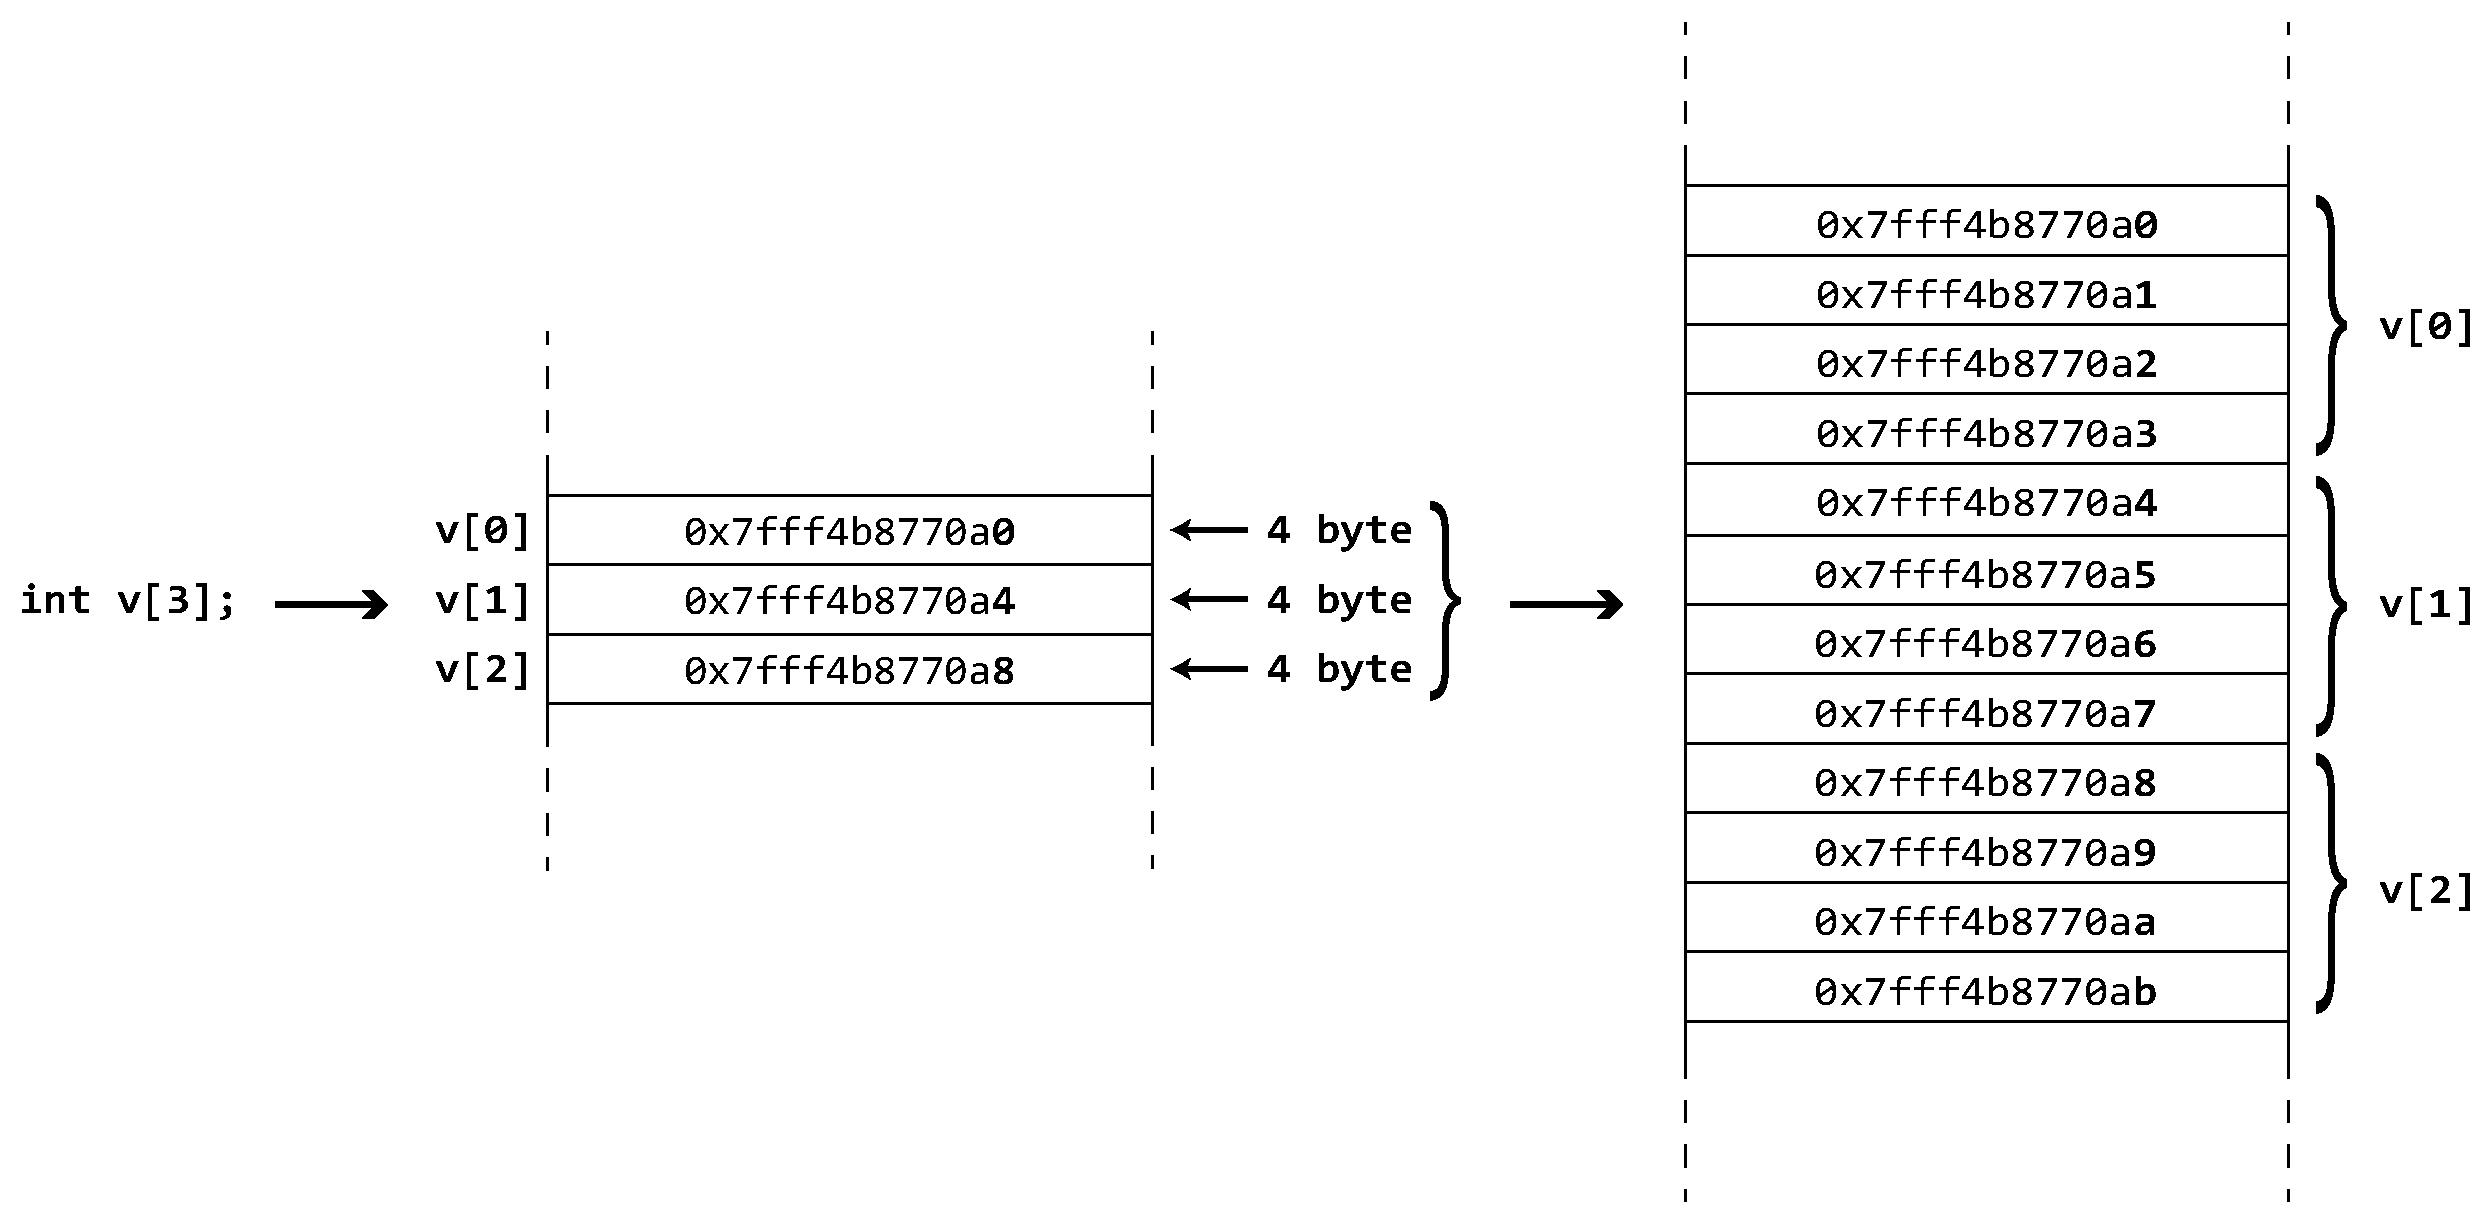
\includegraphics[scale=0.35]{Immagini/array_mem.pdf}  
	\captionsetup{margin=1.5cm} %justification=centering,
	\caption{Rappresentazione di un \emph{array} in memoria. La prima schematizzazione rappresenta gli elementi (\textbf{int}) dell'\emph{array} con i relativi indirizzi. La seconda schematizzazione rappresenta tutti i singoli byte dell'\emph{array}: notare che l'indirizzo di ogni elemento è l'indirizzo del suo primo byte.\protect\footnotemark}
	\label{memory2}
\end{figure}



	Una parte di un esercizio di un tema d'esame (25 febbraio 2014) chiedeva:
\begin{shaded}
Sia
 
\qquad\textbf{int} \verb|w[5];|\\
se l'indirizzo di \verb|w[0]| termina con \verb|1dfd| come terminano gli indirizzi 
di \verb|w[2]| e \verb|w[4]|?
\end{shaded}
Per trovare l'indirizzo di \verb|w[2]|, dobbiamo sommare 8 byte all'indirizzo di \verb|w[0]|, e quindi troviamo $1e16$. Per trovare l'indirizzo di \verb|w[4]|, sommiamo altri 8 byte e troviamo $1e1a$.
\begin{subappendices}
	\section*{COMPLEMENTI}
	\addcontentsline{toc}{section}{COMPLEMENTI}
%\begin{small}
 \footnotetext{Ringrazio Stefano Balzan per la realizzazione dell'immagine.} %va messo qua per avere la nota nella stessa pagina dell'immagine... che schifo...
\section{Architetture a 32 e 64 bit}\label{archCPU}
Questa sezione, per programmare in \verb|C++|, non ha alcuna utilità  pratica, ma può essere interessante a livello ``culturale''.\\

Hai mai sentito parlare di computer a 32 e a 64 bit? 

Il processore comunica con la memoria tramite dei \emph{bus}, che sono veri e propri canali fisici della scheda madre: vi è il \emph{bus} degli indirizzi, il \emph{bus} dei dati e il \emph{bus} di controllo; quest'ultimo, a noi, non interessa. Nel \emph{bus} degli indirizzi viaggia l'indirizzo fisico a cui andare a leggere o scrivere, mentre nel \emph{bus} dei dati passa il dato letto o da scrivere. Ecco, la dicitura ``32 bit'' indica esattamente la dimensione di questi \emph{bus}, oltre alla dimensione di alcune piccolissime memorie interne alla CPU, detti \emph{registri} (la RAM, per la CPU, è lenta: i \emph{registri} sono piccolissime memorie ad accesso praticamente istantaneo utilizzate per scrivere i risultati intermedi di calcoli vari). L'insieme di queste caratteristiche costituisce l'\emph{architettura} della CPU. 

I primi computer avevano \emph{bus} da 8 bit, quindi da 16 (ad esempio Windows 95 era scritto per girare su computer di questo tipo). Poi si è passati a 32 e, più o meno recentemente, sono nate CPU a 64 bit, che oggi predominano il panorama.

Ma cosa cambia tra queste diverse architetture? 

La prima grande restrizione è nel \emph{bus} degli indirizzi. Torniamo alla fine degli anni '90, quando l'architettura maggiormente in voga era il 32 bit. Quanto è grande un indirizzo da 32 bit in base decimale? Una variabile di questa dimensione può immagazzinare numeri che vanno da 0 a 4.294.967.296. Se ogni numero rappresenta un indirizzo di memoria (e, ricorda, ogni indirizzo è un byte), posso indicizzare circa $4\cdot10^9$ byte, ovvero 4 gigabyte. Ecco trovato il primo limite dei 32 bit: un processore di questo tipo non può gestire una RAM più grande di 4 gigabyte\footnote{In realtà ben presto nacque la tecnologia PAE ("Phisical Address Extention") che aggiunge 4 bit agli indirizzi fisici: il sistema operativo riesce così a gestire fino a 64GB di memoria, ma i singoli programmi rimangono limitati a 4GB.}. 

L'altro limite riguarda il \emph{bus} di dati: anche le variabili sono limitate a 32 bit e una CPU di questo tipo non sa gestire in maniera naturale i \textbf{long} e i \textbf{double}.

Ben presto i 32 bit divennero eccessivamente limitanti e, nei primissimi anni duemila, nacque l'architettura a 64 bit:  il primo utilizzatore (e per un po' l'unico) fu Linux. Con i 64 bit la dimensione fisica di entrambi i \emph{bus} fu raddoppiata. Consideriamo gli indirizzi: $2^{64}$ è circa $1.8\cdot10^{19}$, ovvero circa 18 milioni di terabyte ($1.8\cdot10^{10}$ gigabyte, qualcosa di spropositato). Le prime versioni dell'architettura a 64 bit limitarono il \emph{bus} virtuale degli indirizzi a 48 bit: in questo modo sono indicizzabili 256 terabyte di RAM, assolutamente più che sufficienti oggi e, probabilmente, per molti altri anni\footnote{Alla data di scrittura, la maggior parte dei computer portatili sono dotati di 4-16 gigabyte di memoria, i server più potenti arrivano a 128.}.

I diversi sistemi operativi gestiscono questi indirizzi in maniera differente. Linux usa per i processi  47 bit di indirizzi rendendo utilizzabili ``solo'' 128TB (mentre il kernel li può usare tutti e 256). 

Windows, fino alla versione 7, limitava l'uso di solo 8TB di indirizzi virtuali. Dalla versione 8.1 è stato esteso l'uso a 128TB di indirizzi, ma purtroppo non esistono compilatori open-source a 64 bit (il compilatore proprietario Microsoft è a pagamento). Inoltre, a meno di non dare al compilatore l'opzione ``\emph{LARGEADDRESSAWARE}'', tutti i programmi sono limitati a 2 gigabyte (quindi anche meno dei 4GB delle  vecchie CPU da 32 bit\ldots). 

Per quanto riguarda MacOS, ammetto la mia completa ignoranza.

Tornando ai \emph{bus}, rimane da analizzare quello dei dati: a  differenza del \emph{bus} degli indirizzi, viene utilizzato interamente, permettendo di gestire in modo naturale dati da 8 byte (64 bit), cioè i nostri \textbf{long} e \textbf{double}. Ma non è l'unico vantaggio: l'esistenza delle piccole memorie interne alla CPU, anch'esse da 64 bit, permette di lavorare contemporaneamente su due dati da 4 byte (\textbf{float} e \textbf{int}) dimezzando il tempo di calcolo (se il codice macchina istruisce la CPU a farlo), ma questo interessa a chi scrive i compilatori\ldots.
%\end{small}

\end{subappendices}

	
\chapter{Strutture di controllo e cicli}\label{cicli}	
Abbiamo visto buona parte di ciò che concerne i dati e la memoria; siamo capaci di usare le variabili e abbiamo capito come vengono trattate nella RAM. Ma, con gli strumenti che abbiamo, il nostro codice non ha molte potenzialità operative, non è particolarmente versatile. 
	
In questo capitolo studieremo due importantissime strutture che rendono il codice potente e dinamico: le strutture di controllo e i cicli. Dal momento che le prime sono spesso utili nelle seconde, inizieremo con queste.
\section{Strutture di controllo}
Ci sono situazioni in cui l'operazione che desideriamo eseguire cambia in base alle condizioni iniziali. Mi spiego meglio: se all'inizio abbiamo una situazione, potremmo voler fare una determinata operazione; se invece la situazione è un'altra, potremmo desiderare una diversa operazione. Come facciamo? Il nostro codice viene eseguito in maniera consequenziale: un'operazione dopo l'altra (una riga di codice dopo l'altra). Come facciamo a dire: ``No, non eseguire quest'operazione, esegui quella!''?\\
	
Per capire meglio ti propongo un esempio pratico: vogliamo scrivere un programma che, preso in input un numero, ne trovi il valore assoluto. 
	
Se viene inserito un numero negativo, ci basta farne il modulo moltiplicando per $-1$, ma se viene inserito un numero positivo? La moltiplicazione per $-1$ non deve assolutamente avvenire!
	
Cerchiamo di estrapolare i concetti generali. Per prima cosa dobbiamo controllare la situazione iniziale, ovvero se si verifica una condizione specifica: nel nostro caso il segno del numero (ad esempio, per condizione prendiamo la negatività del numero). A seconda che la condizione si verifichi o no, dobbiamo eseguire un'istruzione o l'altra.
	
Tornando al nostro esempio: se il numero è negativo (condizione verificata) allora dobbiamo trovarne il valore assoluto, ma se il numero è positivo (condizione non verificata) allora non dobbiamo eseguire nessuna operazione.\\
	
Nota una cosa: il controllo di una condizione è un'operazione binaria. La condizione è verificata o non è verificata, non esiste una terza opzione. Una variabile booleana è perfetta per rappresentare questa situazione: può essere settata su \textbf{true} se la condizione si verifica, \textbf{false} negli altri casi.\\
\subsection{\emph{if\ldots else}} 
Passiamo ad analizzare il codice che rappresenta questa situazione.
\paragraph{if(\ldots)\{\ldots\}}Esiste un costrutto che, a partire da una situazione iniziale, controlla se una condizione viene verificata.  Quindi, se ciò avviene, entra in un nuovo scope ed esegue ciò che è contenuto.
	
Questo costrutto è il seguente:
\begin{lstlisting}
if(condizione della situazione iniziale){//nuovo scope
	//istruzioni
}
\end{lstlisting}
Nota che \textbf{if} è una parola riservata. ``If'' viene seguito da parentesi tonde: al loro interno vi è un codice (generalmente breve) che controlla la situazione iniziale, questo codice deve produrre un risultato tassativamente booleano. Infatti, se nelle parentesi tonde, a controllo concluso, risulta un valore \textbf{true} allora il programma entra nelle parentesi graffe che seguono; se, invece, si trova un valore \textbf{false} ciò non avviene. \\
	
Per capire meglio l'uso di questo enunciato all'interno di un programma, vediamo un esempio pratico: vogliamo scrivere un programma che decida se è pari un numero inserito da tastiera.
	\begin{lstlisting}
#include <iostream>
using namespace std;

int main(){
	int numero=0;
	cout << "Inserisci un numero: " << endl;
	cin >> numero; //cin legge da tastiera un valore e lo inserisce in numero
	if(numero%2==0){
		cout << "Il numero e' pari!" << endl;
	}
	return 0;
}
\end{lstlisting}

Cosa succede?
Fino a  \emph{cin} dovrebbe esserti tutto chiaro. \emph{Cin}, così come \emph{cout}, è un operatore di input/output (o meglio, \emph{cin} di input, \emph{cout} di output). \emph{Cin} è un'abbreviazione di ``console input'' e legge da tastiera un valore, viene seguito da ``>>'' e da una variabile: scrive il valore inserito da tastiera nella variabile. Per una spiegazione più approfondita vedi il capitolo in/out.

A questo punto interviene \textbf{if}: trova il resto della divisione e lo paragona con zero, e se è uguale a zero (il numero è pari) il confronto restituisce \textbf{true}.  Potremmo dire che, in questo caso, \textbf{if} dà l'ok per entrare nelle parentesi graffe: il codice in esse contenuto viene eseguito. Se il resto della divisione non è zero, il confronto con zero dà come risultato \textbf{false}: \textbf{if} non permette di entrare nelle parentesi graffe e il relativo codice non viene eseguito.\\

Perché ho scritto ``=='' e non un semplice ``=''? Questi due simboli, in realtà, sono profondamente diversi. Il primo è un operatore binario\footnote{Con operatore binario, si intende che necessita di due operandi. Un operatore che lavora su un solo operando è detto ``unario''. Ci tengo a sottolineare che ``binario'' non significa, quindi, che opera sui bit. Un operatore che agisce sui bit è detto ``bit a bit'' o, in inglese, \emph{bitwise} (un operatore binario, invece, è detto \emph{binary}).}, ovvero confronta ciò che è a destra con ciò che è a sinistra: se sono uguali restituisce \textbf{true}, altrimenti \textbf{false}. Il semplice ``='', invece, è un operatore di assegnazione: il valore contenuto nella variabile a destra viene assegnato a quella di sinistra. 

Nella prossima sottosezione approfondiremo gli operatori binari e il loro funzionamento. Prima, però, voglio introdurre il completamento naturale della struttura \textbf{if}.

\paragraph{else\{\ldots\}} Nell'esempio precedente controlliamo se una variabile è pari e stampiamo a video questa considerazione. E se volessimo stampare a video qualcosa anche quando la variabile è dispari?
Potremmo pensare di fare una cosa così (ti avviso, è sbagliato!):
\begin{lstlisting}
#include <iostream>
using namespace std;
	
int main(){
	int numero=0;
	cout << "Inserisci un numero: " << endl;
	cin >> numero; //cin legge da tastiera un valore e lo inserisce in numero
	if(numero%2==0){
		cout << "Il numero e' pari!" << endl;
	}
	cout << "Il numero e' dispari!" << endl;
	return 0;
}
	\end{lstlisting}
Se il numero è dispari il programma non entra nello scope di \textbf{if} e tutto va bene: viene stampata la cosa giusta. Ma se il numero è pari? Abbiamo un problema: non solo il programma entra nello scope di \textbf{if}, ma viene stampato anche ciò che segue. Il risultato ottenuto non è quello desiderato!
Potremmo procedere con un secondo \textbf{if} dove, per condizione, andremmo a controllare la cosa \emph{esattamente opposta}. 
	
Quando dopo un \textbf{if} abbiamo un codice che deve essere eseguito al verificarsi della condizione opposta dell'\textbf{if} iniziale, ci viene in aiuto un'altra struttura (in modo da evitare un secondo e ridondante \textbf{if}): \textbf{else}.

Il codice di prima, corretto, diventa:
	\begin{lstlisting}
#include <iostream>
using namespace std;
	
int main(){
	int numero=0;
	cout << "Inserisci un numero: " << endl;
	cin >> numero; //cin legge da tastiera un valore e lo inserisce in numero
	if(numero%2==0){
		cout << "Il numero e' pari!" << endl;
	}
	else{
		cout << "Il numero e' dispari!" << endl;
	}
	return 0;
}
	\end{lstlisting}
	Come funziona \textbf{else}? Si oppone ad un \textbf{if}. Se la condizione di entrata nell'\textbf{if} non è verificata, allora si entra nello scope dell'\textbf{else} (quest'ultimo, quindi, non ha bisogno di alcuna parentesi tonda contenente una condizione). \`E implicito che un \textbf{else} non ha senso se non è preceduto da un \textbf{if}.
	
	\paragraph{NOTA} Una piccola precisazione: se l'istruzione da eseguire dentro un \textbf{if} o un \textbf{else} è costituita da una singola riga di codice (se e solo se è una sola riga!), allora possiamo evitare le parentesi graffe dello scope. Te lo dico perché, per brevità del codice, spesso nei miei esempi scriverò così. Varrà lo stesso per i cicli, ma lo ripeterò. \\
	
	Ti faccio notare che un \textbf{if} non deve per forza essere seguito da un \textbf{else}. Ci sono casi in cui, se la condizione non si verifica, non deve essere eseguito alcun codice alternativo: un caso è l'esempio del valore assoluto che avevo introdotto all'inizio. A dirla, tutta dovresti essere in grado di scrivere il programma da solo (fallo!), in ogni caso ti riporto una possibile soluzione:
	\begin{lstlisting}
#include <iostream>
using namespace std;

int main(){
	int numero=0;
	cout << "Inserisci un numero: " << endl;
	cin >> numero;
	if(numero<0)
		numero=numero*(-1);
	cout << "Valore assoluto: " << numero << endl;
	return 0;		
}
	\end{lstlisting}
	
	Le strutture di controllo possono essere incluse una dentro l'altra, incastrate in una scalata di \textbf{if} ed \textbf{else}; ad esempio:
	\begin{lstlisting}
#include <iostream>
using namespace std;
int main(){
	int numero=0;
	cout << "Inserisci un numero maggiore di zero: " << endl;
	cin >> numero;
	if(numero<10){
		cout << "Il numero ha una singola cifra." << endl;
		if(numero%2==0){
			cout << "Il numero e' pari. " << endl;
			if(numero==2)
				cout << "Il numero e' primo." << endl;
		}
	}
	
	return 0;
}
	\end{lstlisting}
	
	Non è l'unica situazione dove puoi trovare tanti \textbf{if} e, ovviamente, \textbf{else}: nell'esempio di prima per ogni condizione avrei potuto mettere il complementare dentro un \textbf{else}); l'altra situazione è quella, mi vien da dire, ``a cascata'': tanti \textbf{if} scollegati e uno dopo l'altro.
	
	Ti riporto un esempio molto semplice. Vedremo più avanti che esiste una struttura che è in grado di risolvere la stessa situazione in maniera elegante, ma solo in condizioni molto particolari.
	
	\begin{lstlisting}
#include <iostream>
using namespace std;
int main(){
	int c=0;
	cout << "Inserisci un numero da 1 a 5 corrispondente ad una lettera da 'a' a 'e': " << endl;
	cin >> c;
	if(c==1)
		cout << "a!" << endl;
	if(c==2)
		cout << "b!" << endl;
	if(c==3)
		cout << "c!" << endl;
	if(c==4)
		cout << "d!" << endl;
	if(c==5)
		cout << "e!" << endl;
	return 0;
}
	\end{lstlisting}
		
	\subsection{Operatori binari e logici}
	Abbiamo visto che \textbf{if} vuole, nelle parentesi tonde, un enunciato che produca un valore booleano. La cosa più banale è una variabile \textbf{bool}; questa non è, però, l'unica situazione che produce un risultato booleano: molto più notevoli sono gli operatori binari. 
	
	Gli operatori binari valutano una relazione tra due variabili, e a seconda del risultato restituiscono \textbf{true} o \textbf{false}. Nei codici precedenti ne ho introdotti un paio senza molte spiegazioni: vediamoli in dettaglio. 
	
	Chiedersi se una variabile è maggiore (o minore) di un'altra è una relazione binaria: se la variabile è effettivamente maggiore (rispettivamente minore) allora verrà restituito \textbf{true}, al contrario \textbf{false}. 
	
	
	Esistono operatori binari relativi alla matematica ed operatori puramente logici, vediamoli!
	
	Gli operatori binari matematici che andremo ad utilizzare sono i seguenti (il codice in \verb|C++| segue tra virgolette dopo la freccina):
	\begin{itemize}
	\item \textbf{Uguale} $\to$ \textbf{`` == ''}
		\\Come ho già accennato, c'è una profonda differenza tra ``='' e ``==''. Il singolo uguale è un operatore di assegnazione. Ne abbiamo già discusso, non approfondirò di nuovo il significato. I programmatori del \verb|C|, per distinguere l'operatore logico ``uguale'' dall'uguale di assegnazione hanno deciso che, per il primo, il simbolo sarebbe stato ``==''.\\
		Quest'operatore controlla se ciò che è posto a sinistra coincide con ciò che è posto a destra, in tal caso produce un valore \textbf{true}; se ciò non avviene produce un \textbf{false}.\\
		Stai attento a non confondere ``=='' con ``='': se lo fai combini sicuramente un bel disastro nel tuo codice, hai capito perché?\\ \\
		\emph{Importante}: non usare \emph{mai} quest'operatore tra variabili di tipo \textbf{float} o \textbf{double}. Quando abbiamo studiato i dati in virgola mobile, abbiamo visto che non sempre ritroviamo risultati esatti o quello che ci aspettiamo. Un'operazione che dovrebbe generare ``$0$'', nel computer potrebbe produrre un risultato prossimo a tale valore, ma non esattamente zero!!! 
		\\Ti ricordi l'esempio di codice che ti avevo proposto per farti vedere un caso in cui accade esattamente quel problema? Un programma come quello che segue non funzionerà mai:
		\begin{lstlisting}
#include <iostream>
using namespace std;
int main(){
	float a=0.3, b=0.2, c=0.1;
	float d=a-b-c;
	if(d==0)
		cout << "Risultato corretto! " << endl;
	return 0;	
}
		\end{lstlisting}
		Questo è un programma inutile e stupido, ma se nel tuo codice, scrivendo programmi seri, usi dei numeri in virgola mobile con ``=='' potresti creare errori per nulla facili da individuare. \\
		Usa l'operatore ``=='' solo con \textbf{int}, \textbf{short}, \textbf{long}, \textbf{char} e \textbf{bool}.
	 
	\item \textbf{Diverso} $\to$ \textbf{`` != ''}
	\\Non c'è molto da spiegare: è l'esatto opposto dell'operatore precedente. Il punto esclamativo nega ciò che segue: significa ``non uguale''. Questo operatore confronta ciò che è a sinistra con ciò che è a destra: se differiscono produce un valore \textbf{true}.
	\\Giusto per completezza: esiste una parola riservata per indicare ciò che in simboli è ``!='': \textbf{not\_eq}; non ti capiterà praticamente mai di trovarla, ma nel caso sai cos'è\ldots
	\\Vale la stessa considerazione di prima sul non usare numeri in virgola mobile (anche perché, essenzialmente, quest'operatore è identico al precedente: semplicemente produce risultati opposti).
	
	\item \textbf{Maggiore}  $\to$ \textbf{`` > ''}
	\\Funziona esattamente come il relativo operatore matematico. Inoltre, è molto meno problematico nell'uso con i numeri a virgola mobile dei precedenti operatori: l'unico caso critico è quello in cui, di nuovo, due numeri dovrebbero essere uguali (e quindi restituire \textbf{false}) ma in realtà uno è leggermente maggiore dell'altro. \`E comunque un caso raro e, perciò, è comune usare questo operatore anche con i \textbf{float} e i \textbf{double}.
	\item \textbf{Maggiore o uguale}  $\to$ \textbf{`` >= ''}
	\\Anche in questo caso, stesse funzionalità dell'operatore matematico e quasi nessun problema con i \textbf{float} e i \textbf{double}.
	\item \textbf{Minore} $\to$ \textbf{`` < ''}
	\\Stesse considerazioni fatte per ``>''.
	
	\item \textbf{Minore o uguale}  $\to$ \textbf{`` <= ''}
	\\Stesso discorso del ``>=''.
	\end{itemize}
	
	Abbiamo visto praticamente tutti gli operatori binari matematici. Ci sono, però, ancora due operatori binari, diciamo ``logici'': \emph{and} e \emph{or}.
	
	Questi due operatori, a differenza dei precedenti, a sinistra e a destra hanno dei valori booleani e stabiliscono delle relazioni tra gli stessi restituendo un nuovo valore booleano. Vediamo in dettaglio come funzionano.
	\begin{itemize}
	\item \textbf{and}: se sia a destra che a sinistra vi sono due \textbf{true}; restituisce a sua volta \textbf{true}, se i due valori sono diversi o entrambi \textbf{false}, allora restituisce \textbf{false}.
	\\Nel \verb|C| non esisteva la parola riservata \textbf{and}: il simbolo per rappresentarla era ``\&\&''. Nel codice scritto da qualche nostalgico (o pezzi di codice derivanti dal \verb|C|), potresti trovare questo simbolo: non spaventarti, è un semplice \textbf{and}.
	
	
	\item \textbf{or}: affinché sia prodotto un valore \textbf{true}, è sufficiente che solo uno dei due valori sia \textbf{true} (ovviamente possono esserlo entrambi); per cui, l'unico caso in cui viene prodotto un valore \textbf{false} è quando entrambi sono \textbf{false}.
	\\Anche \textbf{or} non esisteva nel \verb|C|: il relativo simbolo era ``||''.
	
	\item Ti aspettavi due punti e invece ecco il terzo!	Voglio fare una precisazione: ``\textbf{!}'' può essere usato in situazioni diverse dal ``!=''. Lo possiamo usare per negare una qualsiasi operazione che produca un valore booleano. 
	\\Il punto esclamativo è, infatti, un operatore logico vero e proprio che nega ciò che segue ma non è un operatore binario: prende un solo argomento.
	\\Di nuovo, per completezza, sappi che esiste una parola riservata per indicare ``!'': \textbf{not}; ti sarà raro trovarla, ma nel caso\ldots
	\\Se scriviamo:
	\begin{lstlisting}
		if(!( a>0 and a<10))
	\end{lstlisting}
	stiamo imponendo che \verb|a| deve essere minore di 0 e maggiore di 10 (estremi inclusi). In questo caso, avremmo potuto semplicemente invertire i versi. Ci sono situazioni, però, in cui torna comodo (ad esempio per negare il valore che ritornano alcune funzioni, nei prossimi capitoli vedrai qualche esempio).\\
	Ovviamente puoi usarlo per negare anche una semplice variabile booleana, esempio:
	\begin{lstlisting}
	bool var=true;
	if(var)
		//codice
	if(!var)
		//codice
	\end{lstlisting}
	Il programma entra nel primo \textbf{if}, mentre nel secondo no.
\end{itemize}
	\textbf{if}, \textbf{and} e \textbf{or} spesso tornano utili per effettuare dei controlli, potremmo dire di ``sicurezza'', sugli input (e varie altre cose). Ad esempio, nel programma scritto prima in cui si chiedeva un numero da 1 a 5 da convertire in lettera, si potrebbe inserire un ``check'' sul fatto che effettivamente il numero inserito sia compreso tra 1 e 5. Provo a farti vedere:
	\begin{lstlisting}
#include <iostream>
using namespace std;
int main(){
	int c=0;
	cout << "Inserisci un numero da 1 a 5 corrispondente ad una lettera da 'a' a 'e': " << endl;
	cin >> c;
	if(c<1 or c>5){
		cout << "Hai inserito un numero non valido!" << endl;
		return 0; //Con questo comando ritorno al sistema operativo 0, interrompo qui il programma, non continua!
	}
	/* L'if precedente si sarebbe potuto scrivere anche cosi':
	if(!(c>=1 and c<=5)){
		cout << "Hai inserito un numero non valido!" << endl;
		return 0;
	}
	Spesso in informatica esistono piu' modi, ugualmente funzionali, per scrivere la stessa cosa: sta al tuo gusto, e a cosa ti viene in mente prima, decidere come comportarti.
	*/
	if(c==1)
		cout << "a!" << endl;
	if(c==2)
		cout << "b!" << endl;
	if(c==3)
		cout << "c!" << endl;
	if(c==4)
		cout << "d!" << endl;
	if(c==5)
		cout << "e!" << endl;
	return 0;
}
	\end{lstlisting}
	
	\section{Cicli}
	Può capitare di dover compiere istruzioni estremamente ripetitive, tutte uguali o nelle quali cambia veramente poco. Invece di scrivere migliaia di righe di codice, è stato introdotto un utilissimo strumento: il ciclo.
	
	Come funziona un ciclo? \`E composto da due parti: un blocco di codice che viene ripetuto in maniera ciclica e un blocco di codice che valuta una condizione: finché la condizione si verifica (o non si verifica, a seconda del tipo di ciclo) il ciclo continua. 
	
	\`E importante notare una cosa: i cicli sono di tre tipi diversi ma sono sempre intercambiabili. Mi spiego meglio: ognuna delle tre tipologie è più adatta ad alcune situazioni, ma ogni ciclo può essere riscritto usandone un altro. 
	
	A volte ti sembrerà che un problema possa essere risolto con cicli diversi, e non stai sbagliando! \`E veramente così (anche se, in alcune situazioni, alcuni cicli sono molto più adatti di altri). La scelta del ciclo è solo tua: da un lato potresti scegliere quello più elegante (che richiede meno righe di codice), dall'altro seguire la tua inclinazione; io, per esempio, tendo ad abusare del ciclo \textbf{for}, probabilmente mi piace più degli altri!
	
	
	\subsection{\emph{while}}
	Per spiegartelo preferisco partire da un esempio di codice, poi lo analizziamo insieme.
	\begin{lstlisting}
#include <iostream>
using namespace std;
int main(){
	int numero=1; //inizializzo ad uno per poter entrare nel ciclo, vedi la spiegazione
	while(numero !=0){
		cout << "Inserisci un numero (zero per chiudere il programma): ";
		cin >> numero;
		if(numero%2==0) //controllo il resto della divisione
			cout << "E' pari!" << endl;
		else
			cout << "E' dispari!" << endl;
	}
	return 0;
}
	\end{lstlisting}
	In breve, il programma funziona così: si avvia, chiede di inserire un numero, analizza se è pari o dispari e continua così finché non si inserisce zero.
	
	Dovrebbe esserti tutto chiaro nel resto del programma, le uniche perplessità potrebbero essere, giustamente, nel \textbf{while}.
	
	Il ciclo \textbf{while} inizia con la relativa parola riservata, quindi è seguito da una parentesi tonda. All'intero di questa vi è un codice che analizza una condizione, e se come risultato viene prodotto un \textbf{true} si entra nelle parentesi graffe: il codice contenuto in esse viene eseguito. Arrivati alla fine delle graffe, \textbf{while} testa di nuovo la condizione, e così via fino a che non si produce un \textbf{false}. In tal caso non si entra più nelle graffe: il programma procede con ciò che segue oltre il ciclo.
	
	Da notare una cosa: prima di entrare nel ciclo si verifica la condizione, e questo vuol dire che potenzialmente non si potrebbe mai entrare nel ciclo. Nell'esempio precedente, se avessi inizializzato \verb|numero| a zero non saremmo mai entrati nel ciclo \textbf{while} e il nostro programma sarebbe stato decisamente inutile.\\
	
	Torniamo all'esempio. In quel caso, qual era il vantaggio e la necessità di usare un ciclo?
	
	Poniamo che il nostro utente sia così negato per la matematica da avere una quantità di numeri non ben definita da processare per decidere se sono pari o dispari (ironizzo: è un modo per dire che l'informatica non è così stupida, si può scrivere di meglio\ldots Ma come al solito cerco esempi banali per scrivere codici brevi). Abbiamo un problema: quando scriviamo il programma non sappiamo quanti numeri vorrà analizzare l'utente, quindi: o lui per ogni numero riavvia il programma (ma sarebbe un programma terribile, nessuno comprerebbe mai qualcosa del genere!) oppure ci ingegniamo per scrivere un programma che si modifichi a run-time, in base alle necessità dell'utente. 
	
	Ecco qui che entra in gioco il ciclo: potenzialmente il programma va avanti all'infinito, continua a chiedere numeri all'utente da analizzare; è quest'ultimo che interrompe il programma quando è soddisfatto.
	
	Esistono molti altri usi di cicli, alcuni dei quali non dipendono dall'utente, ma da condizioni del computer, o da risultati di calcoli effettuati dal computer. A breve cercherò di presentarti qualche esempio più significativo.\\
	
	\paragraph{Scopes e cicli}
	Una caratteristica comune a tutti i cicli è che ogni singola ripetizione rappresenta uno \emph{scope}. Questo cosa significa? Una variabile dichiarata all'interno delle graffe del ciclo è visibile solo e soltanto in quel singolo \emph{scope}: ad ogni ripetizione nasce, viene usata e alla fine della graffa muore; alla ripetizione successiva, nasce di nuovo. Per cui, se avevi assegnato un valore alla ripetizione precedente, non sarà più visibile!
	
	Questo esempio dovrebbe chiarire:
\begin{lstlisting}
#include <iostream>
using namespace std;

int main(){
	int i=0;
	while(i<10){
		int j=1;
		i=j;
		j++; 	
	}
	return 0;
}
\end{lstlisting}
	Il ciclo non si interrompe mai: \verb|j| ad ogni ciclo rinasce e averlo incrementato alla ripetizione precedente non è servito a nulla\footnote{Se un tuo programma entra in \emph{loop} e lo vuoi interrompere, premi Control+C.}. 
	\subsection{\emph{do\ldots while}}
	Nel ciclo \textbf{while}, come abbiamo visto, prima di entrare nelle graffe viene testata la condizione, in questo modo non è detto che si entri nel ciclo. 
	
	Potremmo desiderare, a volte, che avvenga il contrario: per prima cosa si entri, almeno una volta, nel ciclo, dopo di che, per decidere se entrarci di nuovo, dobbiamo testare la condizione, e così via.
	
	Riprendiamo l'esempio di prima: affinché si entrasse nel \textbf{while} abbiamo dovuto inizializzare la variabile \verb|numero| al valore di uno. Dopo un po' che si programma, nel corso di Informatica 1, inizia a diventare automatico inizializzare le variabili numeriche a zero; ricordarsi di inizializzarla ad un valore diverso può essere non del tutto banale. Insomma, tutto questo  per dire: non sarebbe più comodo inizializzare la variabile a zero ed avere un ciclo che, almeno una volta, chiede all'utente di inserire un numero e poi testa la condizione?\\
	
	Esiste il ciclo \textbf{do\ldots while}; riscrivo il programma di prima utilizzandolo, poi, come al solito, spiego tutto.
	
	\begin{lstlisting}
#include <iostream>
using namespace std;
int main(){
	int numero=0;
	do{
		cout << "Inserisci un numero (negativo per chiudere il programma): ";
		cin >> numero;
		if(numero%2==0) //controllo il resto della divisione
			cout << "E' pari!" << endl;
		else
			cout << "E' dispari!" << endl;
	}while(numero >=0);
	return 0;
}
	\end{lstlisting}
	Il programma, arrivato alla parola riservata \textbf{do}, entra nel ciclo, esegue il codice e, solo successivamente, arriva al \textbf{while}, dove testa la condizione e decide se entrare in un nuovo ciclo.
	
	Ti faccio notare una differenza rispetto al ciclo \textbf{while}: nel \textbf{do\ldots while} è \emph{necessario}, alla fine, un bel punto e virgola! \\
	
	Per concludere: i due cicli analizzati finora sono estremamente simili, la differenza è che il secondo esegue almeno una volta il codice tra le graffe.\\
	
	Come accennato, i vari cicli sono interscambiabili. Se vuoi fare un esercizio, per convincerti, prova a scrivere quest'ultima versione del programma (con \verb|numero| inizializzato a 0) con un ciclo \textbf{while}. Dovrai inserire qualcosa di nuovo: prima, dentro o dopo? E cosa?	
	
	\subsection{\emph{for}} 
	Passiamo all'ultimo ciclo, il quale, apparentemente, è tutta un'altra cosa. Un esempio:
\begin{lstlisting}
#include <iostream>
using namespace std;
int main(){
	unsigned int num=0;
	cout << "Programma per conto alla rovescia, da che numero vuoi partire?: ";
	cin >> num;
	for(int i=0; i<num; i++){
		cout << num-i << endl;
	}
	cout << "Zero!" << endl;
	return 0;
}
\end{lstlisting}
	Il ciclo \textbf{for} è composto da due parti: una parentesi tonda e la solita parentesi graffa con il codice da eseguire.
	
	La parentesi tonda, però, è profondamente diversa da quelle degli altri due cicli, vediamo perché.
	
	Come puoi notare, vi sono tre parti distinte separate da un punto e virgola. La prima parte serve per dichiarare ed inizializzare una variabile, detta contatore; generalmente viene chiamata \verb|i|, ma puoi chiamarla come vuoi (se hai tanti \textbf{for} uno dentro l'altro, devi per forza dare nomi diversi); io l'ho inizializzata a zero, ma il valore può essere qualsiasi (spesso si sceglie un valore comodo e sensato per quello che dobbiamo fare). La seconda parte è quella in cui viene testata la condizione, nello specifico che la nostra \verb|i| sia minore di \verb|num|: finché ciò si verifica le iterazioni continuano. La terza parte effettua un'operazione sulla variabile contatore: per esempio io l'ho incrementata (specifico: ad ogni iterazione viene incrementata).
	
	Il concetto è che \verb|i| parte da 0 e ad ogni iterazione si incrementa di 1. Quando arriva al valore \verb|num|-1 (e quindi il programma può ancora entrare nel ciclo) \verb|i| viene incrementato di 1: al successivo controllo non è più minore di \verb|num|, così si esce dal ciclo \textbf{for}.
	
	A volte, le variabili contatore partono da un valore, tipo 10, e vengono decrementate; insomma, non per forza dobbiamo incrementarla! 
	
	Ti accorgerai dell'utilità dei cicli, in particolare del \textbf{for}, parlando di \emph{array}.
	
	Ti faccio notare che, così come con gli \textbf{if}, se abbiamo una sola riga di codice, anche nei cicli possiamo evitare le parentesi graffe.\\
	
	Ora come ora, probabilmente, ti sarà difficile vedere come il ciclo \textbf{for} possa essere equivalente agli altri due. Per capirlo ci serve uno strumento molto utile: il \textbf{break}.
	\subsection{Gli enunciati \emph{break} e \emph{continue}}
	Abbiamo visto che tutti i cicli controllano \emph{una} condizione, solo una! E se noi volessimo controllarne un'altra? Se all'accadere di un particolare evento (uno nuovo, non la condizione del ciclo) volessimo interrompere il ciclo?	\`E possibile: la combinazione di un \textbf{if} e un enunciato \textbf{break} lo permette.
	
	Quando in un ciclo il programma incontra un enunciato \textbf{break}, a qualsiasi iterazione si trovi, il ciclo viene interrotto, si esce dallo \emph{scope} e si continua nel codice del programma.
	
	Un \textbf{break} può essere davvero utilissimo: possiamo usarlo come controllo sulle iterazioni del ciclo (ad esempio interromperlo se dura troppo), oppure per interruzioni forzate da parte dell'utente, ecc\ldots \\
	
	Propongo un esempio: è un programma per calcolare il fattoriale di un numero. Quest'operazione è molto delicata, perché genera numeri enormi con una facilità notevole. Per non rischiare l'overflow possiamo inserire un check nel ciclo: quando il nostro calcolo raggiunge una determinata cifra lo interrompiamo.
	\begin{lstlisting}
#include <iostream>
using namespace std;

int main(){
	unsigned int num=0; //unsigned per avere numero massimo piu' grande!
	unsigned int appo=0; //creo una variabile d'appoggio per il calcolo
	cout << "Inserisci un numero di cui calcolare il fattoriale: ";
	cin >> num;
	appo=1; //per il calcolo del fattoriale
	for(int i=1; i<=num; i++){
		appo=appo*i;
		if(appo>=100000000){ //scelgo questo numero perche' mi sembra ragionevole rispetto alle dimensioni della variabile
			cout << "Numeri troppo grandi!" << endl;
			break;
		}
		if(i==num) //se abbiamo incontrato il break questo non viene eseguito mai
			cout << num << "! = " << appo << endl;
	}
	return 0;
}
	\end{lstlisting}
	Ti accorgerai, se provi a compilare il programma, che con numeri molto piccoli superiamo già il limite imposto.
	
	Potremmo scrivere un controllo sull'overflow decisamente migliore, che ci permetta di utilizzare i limiti dell \textbf{unsigned int} fino in fondo. Se hai voglia, te lo lascio per esercizio!\\ \\
	
	%TODO altro esempio?
	
	Passiamo ora al \textbf{continue}. In realtà è molto più raro da usare, trova molte meno applicazioni, e sinceramente nel corso di Informatica 1 non l'ho mai visto usare. Comunque, io te l'accenno: non si sa mai che tu lo possa trovare utile in qualche tuo codice.
	
	L'enunciato \textbf{continue} dice: interrompi questa iterazione, non continuare con il codice nello scope del ciclo, e vai all'iterazione successiva. In poche parole, a differenza del \textbf{break} non interrompe il ciclo, ma solo la singola iterazione dove viene incontrato: fa passare il programma alla successiva.
	
	Un esempio molto semplice:
	\begin{lstlisting}
#include <iostream>
using namespace std;
int main(){
	int salta=0;
	cout << "Inserisci un numero da 1 a 10: quale numero vuoi saltare nel conto alla rovescia? " ;
	cin >> salta;
	for(int i=10; i>0; i--){
		if(i==salta)
			continue;
		cout << i << endl;
	}
	cout << "Zero! " << endl;
	return 0;
}
	\end{lstlisting}
	
	
	Visti questi elementi, ti è più chiaro come un \textbf{for}, insieme ad un \textbf{if} e \textbf{break}, possa sostituire un \textbf{while}? Fai qualche prova!

	\subsection{I cicli infiniti} 
	Un particolare ciclo è il cosiddetto ``ciclo infinito''. Un ciclo che, in teoria, non si interrompe mai: non esiste una condizione di uscita. O meglio: non esiste come condizione inclusa nel ciclo, ma esiste tramite un \textbf{if}-\textbf{break}. 
	
	I cicli infiniti sono utili quando a priori non sappiamo quanti cicli dovremo fare, oppure se le condizioni di uscita sono tante (e di pari importanza). 
	
	Possiamo scrivere cicli infiniti sia usando \textbf{for} che \textbf{while} (e, ovviamente, \textbf{do\ldots while}):
	\begin{lstlisting}
	//Ciclo for infinito
	for( ; ; ){
		espressione da eseguire;
		if(condizione di uscita)
			break;
		if(altra condizione di uscita)
			break;
		... //Altre condizioni?	
	}
	
	//Ciclo while infinito
	while(true){
		espressione da eseguire;
		if(condizione di uscita)
			break;
		if(altra condizione di uscita)
			break;
		... //Altre condizioni?		
	}
	\end{lstlisting}
	
	Ho messo più condizioni per rendere chiaro che possono essere tante, in realtà ne basta una sola (ma almeno una\ldots se no, buona attesa per la fine del programma!).
	
	Il ciclo \textbf{for} infinito ha un vantaggio: può implementare in maniera elegante un contatore di iterazioni. Ti mostro:
	\begin{lstlisting}
	for(int i=0; ; i++){
		espressione;
		if(condizione di uscita)
			break;	
	}
	\end{lstlisting}
	
	Mancando la parte centrale del \textbf{for}, non vi è un limite alle iterazioni; la presenza della variabile \verb|i|, invece, serve da contatore: può essere utile all'interno del ciclo.
	
	Ovviamente, in tutti questi cicli, l'\textbf{if} non deve essere per forza alla fine, ma lo puoi posizionare all'inizio, in mezzo, dove vuoi!\\
	
	Passiamo al dovuto esempio di codice:
	\begin{lstlisting}
#include <iostream>
using namespace std;
int main(){
	const int numero=17;
	int risposta=0;
	cout << "Indovina il numero segreto! Prova con un numero da 1 a 20. Inserisci 0 per chiudere il programma." << endl;
	for( ; ; ){
		cout << "Inserisci un tentativo: ";
		cin >> risposta;
		if(risposta == 0)
			return 0; //chiudo direttamente il programma
		if(risposta == numero)
			break; //interrompo il ciclo infinito
		cout << "Hai sbagliato, prova di nuovo! " << endl;
	}
	cout << "Bravo, hai indovinato! " << endl;
	return 0;
}
	\end{lstlisting}
	Come vedi, posso uscire da un ciclo non solo con l'enunciato \textbf{break}, ma anche con un \textbf{return} (che, in questo caso, chiude il programma).
	
	L'utilità del ciclo infinito, in questo caso, è che abbiamo due condizioni di uscita di pari importanza. \`E, in realtà, una pura questione di stile: avremmo potuto scrivere un normalissimo \textbf{while} e un ulteriore \textbf{if} per la seconda condizione di uscita. Sta sempre a te decidere come comportarti (anche se ci sono occasioni in cui il ciclo infinito è davvero più comodo)!
	
	Dovrebbe essere tutto chiaro, così come il fatto che possiamo complicare il programma inserendo un \textbf{if} per controllare che l'input sia effettivamente un numero tra 0 e 20 ed avvertire l'utente in caso contrario.
	
	\subsection{\emph{switch}\ldots\emph{case}}
	Questo costrutto schematizza una serie di \textbf{if}. Si presta per risolvere in maniera elegante alcune situazioni particolari. 
	
	Ad esempio, se abbiamo una variabile che può assumere valori discreti e per ogni valore vogliamo accada una cosa diversa, lo \textbf{switch-case} è perfetto! \`E un costrutto che si presta benissimo per situazione di ``multi selezione''. 
	
	Ma come è strutturato? In generale è composto così:
	\begin{lstlisting}
	switch(variabile){
		case valore-intero-1:
			espressione;
			break;
		case valore-intero-2:
			espressione;
			break;
		...
		...
		...
		case valore-intero-n:
			espressione;
			break;
		default:
			espressione;	
	}
	\end{lstlisting}
	
	Subito dopo \textbf{switch} vi è una parentesi tonda, all'interno della quale c'è la variabile che può assumere una serie di valori discreti. Segue una parentesi graffa, in cui abbiamo diversi \textbf{case}, uno per ogni valore. Dopo ogni \textbf{case}, infatti, vi è il valore, che può essere o un numero intero o una lettera (la quale va racchiusa tra singoli apici, come `a'). Nota che, quello che segue a \textbf{case}, deve essere un valore costante: non può essere un'espressione del tipo "\verb|nuovavariabile|/17" (che dipende dal valore, variabile, di \verb|nuovavariabile|). Il valore viene concluso da due punti, dopo i quali vi è l'espressione che vogliamo venga eseguita. Alla fine vi è un \textbf{break}: la sua presenza ci porta alla fine della parentesi graffa.  Senza di lui passeremmo al \textbf{case} successivo, anche se non è quello desiderato.
	
	Particolare è la presenza del \textbf{default}: se la variabile assume un valore diverso da quello di ogni \textbf{case}, viene eseguito il codice che segue al \textbf{default} (può anche non seguire niente, se non vogliamo venga eseguito qualcosa).
	
	Questa struttura è particolarmente comoda per menù o situazioni di scelta multipla.
	
	Ti ripropongo il programma per stampare a video le lettere che avevo presentato con l'\textbf{if}. L'ho scritto utilizzando molti elementi presentati finora: ciclo \textbf{for} infinito, \textbf{break} e \textbf{continue}. Dai un occhio: spero ti sia tutto chiaro!
	\begin{lstlisting}
#include <iostream>
using namespace std;
int main(){
	int c=0;
	for( ; ; ){
		cout << "Inserisci un numero da 1 a 5 corrispondente ad una lettera da 'a' a 'e': ";
		cin >> c;
		switch(c){
			case 1:
				cout << "a!" << endl;
				break;
			case 2:
				cout << "b!" << endl;
				break;
			case 3:
				cout << "c!" << endl;
				break;
			case 4:
				cout << "d!" << endl;
				break;
			case 5:
				cout << "e!" << endl;
				break;
			default:
				cout << "Hai inserito un numero non ammesso, inserisci di nuovo!" << endl;
				continue; //passo alla successiva iterazione del for: evito il break di uscita
		}
		break; //sono uscito correttamente dallo switch: interrompo il for infinito!
	}
	return 0;
}
	\end{lstlisting}
	In questo caso, non sappiamo quante volte l'utente sbaglierà ad inserire il numero: finché questo non è corretto dovremo continuare a chiederglielo. Un ciclo infinito si presta molto bene a questa situazione! Nel caso tutto vada bene, alla fine dello \textbf{switch}, vi è un \textbf{break} che interrompe il ciclo infinito. Se, invece, le cose non vanno come dovrebbero, nel \textbf{default} vi è un \textbf{continue} che fa saltare il \textbf{break}: si passa all'iterazione successiva!
	
	
	Avremmo potuto usare, al posto di un ciclo infinito, un \textbf{while} con, come condizione, un controllo sul numero inserito: finché rimane diverso da quelli ammessi, continuano le iterazioni. Questi sono modi diversi per scrivere lo stesso programma, ma l'ho detto: a me piace il ciclo \textbf{for}\ldots


		
	\chapter{Puntatori}
	%TODO vedere indirizzi memoria esame con puntatori
	Un puntatore è un altro tipo di dato, ma è molto particolare: mentre gli \textbf{int} contengono interi, i \textbf{float} numeri in virgola mobile e così via, i puntatori contengono \emph{indirizzi di memoria}. Esistono più tipologie di puntatori, uno per ogni tipo di dato già definito. Un altro modo di immaginarli, infatti, è come una variabile che ``punta'' all'area di memoria occupata da un'altra variabile. Per questo motivo esistono puntatori ad \textbf{int}, puntatori a \textbf{float}, a \textbf{char}, in realtà a qualsiasi tipo di dato esistente (sia quelli standard, che quelli definiti dall'utente; un esempio lo vedrai nel capitolo \ref{struct}).
	
	Per istanziare una variabile puntatore ad uno specifico tipo di dato è necessario apporre un ``\textasteriskcentered'' dopo il tipo di dato. 
	\begin{lstlisting}
int main(){
	int a; //a e' un intero
	int* b; //b e' un puntatore ad intero

	reuturn 0;
}
	\end{lstlisting}
	
	Prima di procedere possiamo farci una domanda: ma quanta memoria occupa un puntatore? Un puntatore ad \textbf{int} occupa lo spazio di un \textbf{int}, quello di un \textbf{char} lo spazio di un \textbf{char} e così via? La risposta è assolutamente no. 
	
	Per quanto esistano diversi tipi di puntatori (e successivamente cercheremo di capire perché) occupano tutti lo stesso spazio: ovvero quanto è necessario per rappresentare un indirizzo di memoria. In un sistema operativo a 32 bit gli indirizzi di memoria occupano proprio 32 bit (4byte), mentre in un sistema operativo a 64 bit occupano proprio 64 bit (8 byte). Ormai, tutti i computer hanno sistemi operativi a 64 bit, per cui possiamo assumere che i puntatori occupano, di norma, 8 byte. 
	

	Se vuoi controllare prova ad eseguire questo:
	
	\lstinputlisting[ label=punt2]{codice/puntatori/p1.cpp}
	
	Nell'esempio \ref{punt2} ci sono un po' di cose nuove, che non riguardano i puntatori. La prima che noterai è il particolare uso di \emph{cout}: si può ``spezzettare'' (usarlo così serve per una maggiore leggibilità del codice: tutto sulla stessa riga diventa pesante!).
	
	L'altra cosa nuova è l'operatore ``\textbf{sizeof}'': come puoi immaginare, restituisce la dimensione della variabile alla sua destra. Oltre che sulle variabili, lo puoi utilizzare anche sui tipi di dato, ma sono necessarie le parentesi: ``\textbf{sizeof}(\textbf{int})''. L'esempio \ref{caratt} è stato ottenuto proprio con questo operatore.
	
	\section{L'operatore ``\&''}
	Bene, ma come si assegna ad un puntatore un indirizzo di memoria? 
	
	Finora, tranne quando ti ho spiegato come sono fatti gli indirizzi di memoria, non ci siamo mai trovati a maneggiarli. Esiste un operatore, ``\&'', la cui funzione è quella di restituire l'indirizzo di memoria della variabile che segue. 
	
	\lstinputlisting{codice/puntatori/p2.cpp}\label{pt1}
	Prima di analizzare il codice ritengo significativo dare un occhio all'output:
	\begin{shaded}
	\begin{verbatim}
		Valore di n:12 				
		Indirizzo di n:	0x7ffd746cc36c
		Valore di p: 0x7ffd746cc36c     
		Indirizzo di p:	0x7ffd746cc360
	\end{verbatim}
	\end{shaded}
	Nel codice ho scritto ``\verb|p=&n|'', ovvero ho assegnato l'indirizzo di ``n'' a ``p'' (il che è lecito, visto che quest'ultimo è un puntatore a float, una variabile che contiene indirizzi di float). Se osservi l'output noterai che indirizzo di ``n'' e valore di ``p'' sono proprio uguali. 
	
	Nell'ultima riga ho voluto far notare che pure ``p'' ha un indirizzo, che è diverso dal suo valore. Nulla vieta, dunque, di ipotizzare l'esistenza di un puntatore ad un puntatore\ldots Ma è un altro discorso: avremo modo di analizzare questo fatidico oggetto più avanti, parlando di matrici.
	
	\section{Dereferenziare i puntatori: l'operatore \textasteriskcentered}
	Se i puntatori avessero la sola utilità di immagazzinare indirizzi di memoria, sarebbero decisamente di scarso interesse\ldots Ci deve essere un qualche modo per dire ``vai a leggere l'area di memoria a cui punti''. E in effetti esiste: è l'operatore ``\textasteriskcentered''.
	
	Scrivo un breve codice, per poi trarre spunto nella spiegazione:
	\lstinputlisting{codice/puntatori/p4.cpp}

	Dove l'output è:
	\begin{shaded}
		\begin{verbatim}
			valore di a: 1
			Indirizzo di a: 0x7ffd77a24f64
			Valore p1: 0x7ffd77a24f64
			Valore dell'oggetto puntato da p1: 1
			Valore di a: 4
			
		\end{verbatim}
	\end{shaded}

	Analizziamo punto per punto:
	\begin{itemize}
		\item \textbf{int *p2} Anche questa scrittura è corretta. Mettere l'asterisco vicino alla variabile o al tipo di puntatore è una questione, quasi sempre, di gusto. Forse la scrittura ``\lstinline|int* p|'' rende più chiara una cosa: così come in ``\lstinline|int n|'' \textbf{int} è il tipo di dato mentre ``n'' è la variabile vera e propria, in un puntatore il tipo di dato è ``\textbf{int*}'' e ``p'' è la variabile. L'asterisco fa parte del tipo di dato, non della variabile. C'è solo un caso in cui si è costretti a porre l'asterisco vicino alla variabile e non al tipo di dato:
		
		\quad \lstinline|int *p1, *p2, *p3;|
		
		Ovvero, quando sulla stessa riga dichiariamo più puntatori: bisogna esplicitare che anche p2 e p3 sono puntatori ad intero. La scrittura ``\lstinline|int* p1, p2, p3;|'' fa si che vengano istanziati, invece, un puntatore ad intero e due interi (rispettivamente p1 e p2,p3).
		
		\item \textbf{p1=\&a} Come già visto, stiamo assegnando l'indirizzo di \verb|a| al puntatore \verb|p1|, e questo dovrebbe rendere chiaro che la variabile è proprio ``\verb|p1|'' e non \verb|*p1| (abbiamo sulla sinistra un puntatore ad intero, sulla destra un indirizzo di un intero: stesso tipo di dato, assegnazione lecita).
		
		\item \textbf{cout << *p1} Ecco qui l'altro uso fondamentale di ``\textasteriskcentered'': quello di operatore per dereferenziare un puntatore. Spiego subito i paroloni. L'operatore ``\textasteriskcentered'', posto prima di una variabile puntatore, significa ``accedi all'area di memoria puntata''. Essenzialmente stiamo leggendo l'area di memoria riservata ad ``int a'', la variabile iniziale; *p, ora, \emph{è} la variabile iniziale (``*p'', non ``p''!), è quella stessa identica cella di memoria, nulla di differente. 
		
		Ora, dovrebbe essere chiaro perché il tipo di dato non è semplicemente \textbf{*} bensì è \textbf{int*}: utilizzando l'operatore di dereferenziazione, come potrebbe sapere il computer \emph{quanta} memoria andare a leggere? Ricordati: ogni byte della memoria ha un indirizzo, e se un puntatore contiene un indirizzo, quest'ultimo è quello del \emph{primo} byte della variabile puntata. Ma, come ben sai, spesso le variabili occupano ben più di un byte: gli int, ad esempio, ne occupano quattro. Per cui, se ``p'' è un puntatore ad interi e scriviamo ``\lstinline|cout << *p << endl|'' il computer sa che deve andare all'indirizzo contenuto in ``p'' e, dato che punta ad un intero, deve leggere quattro byte. Se ``p'' fosse stato un puntatore a double, il computer avrebbe letto otto byte, e così via. 
		
		\item \textbf{*p1=4} Cosa succede? Ormai l'avrai capito meglio di me: il computer sta scrivendo il valore ``4'' nell'area di memoria puntata da ``p1''. Non deve stupire, quindi, che quando successivamente stampiamo il valore di ``a'' quest'ultimo è proprio  ``4''.
	\end{itemize}
	
	È chiaro, quindi, che i puntatori possono essere ``a qualsiasi tipo di dato'': esistono sia puntatori ai tipi di dato standard, che a tipi di dato definiti dal programmatore (ne vedremo un esempio nel capitolo sulle struct); esistono perfino i puntatori a puntatore (alla fine anche lui è una variabile che occupa un'area di memoria ma, come accennato, ne riparleremo prossimamente\ldots); ecco alcuni esempi:
	\begin{lstlisting}
....
char* c;
float* f;
bool* b;
int** i; //puntatore a puntatore ad int, fai finta di non aver visto niente, li studieremo poi...
....
	\end{lstlisting}
	
	Rimane un'ultima cosa da dire: e come si inizializza un puntatore a ``zero''? Come si dice ``non puntare da nessuna parte''? È semplice: si utilizza la parola chiave ``NULL''. Un esempio:
	
	\lstinputlisting{codice/puntatori/p5.cpp}
	L'unico commento necessario è che, dopo aver assegnato un puntatore a ``NULL'', cercare di accedere all'area di memoria puntata non ha alcun senso (come accedo al niente?): se provi ad eseguire il codice noterai, infatti, che il programma va in segmentation fault.\\

	I puntatori, per ora, ti possono sembrare uno strumento astratto e poco utile,  ma vedremo che la loro potenza è ben maggiore del poter semplicemente avere più variabili che si riferiscono allo stesso indirizzo di memoria. Essi mostrano tutta la loro forza con gli \emph{array} e l'\emph{allocazione dinamica} (capitolo \ref{array}) e con le funzioni (capitolo \ref{funzioni}). 
	\chapter{Array e Matrici}\label{array}
Dobbiamo scrivere un programma per analizzare i dati di un esperimento: stiamo misurando una grandezza e per questioni di statistica vogliamo ripetere la misura mille volte, quindi procedere all'analisi dati. Il nostro programma dovrà gestire mille dati. Con le conoscenze informatiche acquisite finora dovremmo scrivere qualcosa di questo tipo:

\begin{lstlisting}[label=esdati]
#include <iostream>
using namespace std;

int main(){
	float a, b, c,...; //Mille float
	//Per non parlare poi del riempimento dei dati:
	a=2.1;
	b=5.3;
	...
	...
	
	//Fosse necessaria la media avremmo bisogno di:
	float media=a+b+c+.......;
	media/=1000.;

	return 0;
}
\end{lstlisting}

In poche parole qualcosa di impossibile, o se non altro completamente inutile (allora tanto vale usare carta e penna\ldots).

Se cerchiamo sul dizionario la parola ``array'' troviamo traduzioni del tipo: ``schieramento'', ``insieme'', ``disposizione''. Un insieme? Schieramento? I nostri mille dati, tutti dello stesso tipo, cos'altro sono se non proprio questo?
	

Ecco, un \emph{array} è uno ``schieramento'' di dati tutti dello stesso tipo: in poche parole, un ``vettore''. Nel capitolo sulla rappresentazione in memoria (capitolo \ref{mem}) ho presentato una breve introduzione, orientata alla loro struttura nella memoria; in ogni caso, facciamo un breve riassunto dei concetti presentati. 

Un \emph{array} è un insieme contiguo in memoria di elementi dello stesso tipo. Cosa vuol dire ``contiguo''? Nella memoria gli elementi sono ``uno dopo l'altro'', non sparsi ma ben ordinati. Se abbiamo un \emph{array} di dieci interi, il compilatore ci assicura che essi occuperanno un blocco di memoria unitario, in cui il secondo elemento segue immediatamente il primo e così via.

\section{Array statici}
Il primo tipo di \emph{array} che incontriamo è l'\emph{array statico}. Un \emph{array} statico è una collezione di elementi dello stesso tipo, la cui dimensione è definita a priori nel codice e che non può cambiare a ``run-time'' (ovvero durante l'esecuzione del programma).

Come al solito, partendo da un esempio di codice, cerchiamo di capire come funzionano gli \emph{array} statici. Il programma \ref{esdati} potrebbe assumere la seguente forma con gli \emph{array}:

\begin{lstlisting}
#include <iostream>
using namespace std;

int main(){
	float dati[1000]; //Dichiaro un array di float di 1000 elementi
	
	
	for(int i=0; i<1000; ++i){
		dati[i]=... //un qualche codice che riempie i dati. Nel capitolo su In/out impareremo a leggere da file, i dati dell'esperimento potrebbero essere in un file
	}
	
	float media=0;
	for(int i=0; i<1000; ++i)
		media+=dati[i];
	
	media/=1000;
	cout << "Media: " << media << endl;
	
	return 0;
}
\end{lstlisting}

Prendendo spunto da questo codice, vediamo le caratteristiche principali degli \emph{array}.
\subsection{Dichiarare array}

Nella prima riga del \emph{main} vi è ``\lstinline|float dati[1000]|'': stiamo dichiarando un \emph{array} di \textbf{float} di mille elementi. Il nome della variabile \emph{array} di \textbf{float} è ``\verb|dati|''. 
	
Un array può essere di qualsiasi tipo di dato: \textbf{float}, \textbf{double}, \textbf{char}, \textbf{bool}, \textbf{int}, ecc\ldots Il numero di elementi è racchiuso nelle parentesi quadre che seguono il nome dell'\emph{array}; è importantissimo notare che questo numero deve essere definito a ``compile-time'': il compilatore deve sapere quanto sarà grande l'\emph{array}, per cui tra le quadre non possiamo mettere variabili che vengono modificate durante l'esecuzione del programma. Sono ammessi, invece: macro, variabili \textbf{const} (entrambi non si modificano durante l'esecuzione) o semplicemente numeri. Perché dovremmo usare una macro o una variabile \textbf{const}? Per comodità: poniamo di sapere che il nostro programma lo compileremo più volte, cambiando sempre il numero di dati che vogliamo analizzare. Se ogni volta dobbiamo modificare il ``1000'' in tutti i punti del codice in cui compare, diventa assai laborioso. Definendo una macro o una variabile \textbf{const} la questione si semplifica:
	\begin{lstlisting}
#include <iostream>
//definisco una macro
#define N 100
using namespace std;
//Alla riga della macro e' equivalente la seguente
//const int N=100; e, come spiegato nel relativo capitolo, ha i suoi vantaggi

int main(){
	float dati[N]; //N non cambiera' mai nell'esecuzione del programma, sia che si usi la macro sia che si usi il const int, quindi e' accettabile per un array statico
	
	for(int i=0; i<N; ++i)
		...
	...
	...
	return 0;
}
	\end{lstlisting}
	
Ogni volta che vogliamo ricompilare il nostro programma cambiando la dimensione dell'\emph{array}, ci basta cambiare la macro (o variabile \textbf{const}): di conseguenza cambierà la dimensione dell'\emph{array}, i cicli \textbf{for}, e tutti i punti in cui N ci serve, senza dover modificare ulteriormente il codice.

Riassumendo:
\begin{lstlisting}
#include <iostream>
#define N 10
int main(){
	const int n=25;
	bool b[n]; 	//array di 25 elementi di bool
	float f[N]; 	//array di 10 float
	double d[50];	//array di 50 double
	int dim=...	//codice che a run time determina il valore di dim
	int array[dim];	//ERRORE! La dimensione non puo' essere determinata a run time
	return 0;
}
\end{lstlisting}
\paragraph{Gli array vanno inizializzati!} Quando dichiariamo un \emph{array} il compilatore ci assicura soltanto di riservare un'area contigua di memoria. Quest'ultima, però, non è inizializzata. Ti ricordi? C'è dentro ``sporcizia'', valori a caso. Per cui, quando dichiari un \emph{array}, ricordati di inizializzarlo: riempilo dei valori che ti servono, o utilizza un ciclo \textbf{for} per, ad esempio, inizializzare tutti gli elementi a zero. 
\subsection{Indici e\ldots out of range!}
Scrivendo \textbf{dati[i]=...} stiamo richiamando l'i-esimo elemento del nostro \emph{array}. Nota una cosa e imprimitela benissimo in testa: negli esempi di codice, l'indice del ciclo \textbf{for} parte da zero. Questo non è un caso: l'indicizzazzione degli \emph{array} parte proprio da zero! Il primo elemento è ``\verb|dati[0]|'', il secondo è ``\verb|dati[1]|'  e, se N è la dimensione dell'\emph{array}, l'ultimo elemento è ``\verb|dati[N-1]|. E se scrivo ``\verb|dati[N]|''? Semplicemente ``esco dall'\emph{array}''. Stai molto attento: nel \verb|C++| non vi è alcun controllo sui limiti degli indici, né a run-time, né tanto meno a compile-time. Per cui cosa accade? L'\emph{array} è un'area contigua di elementi di memoria, e scrivere ``\verb|array[x]|'' mi fa accedere ad un elemento, ma se sforo l'indice il programma si sposta oltre: accede alle aree di memoria successive. C'è un problema: queste aree di memoria non sono dell'\emph{array} e, spesso, non sono neanche del programma. Sforare i limiti dell'\emph{array} ti fa leggere dati senza alcun senso, o ti fa scrivere in zone non tue: se non sono neanche del programma il sistema operativo ti ``uccide''\footnote{Almeno per quanto riguarda i sistemi Unix.}, cioè molto semplicemente non ti lascia scrivere nella memoria che non ti appartiene e il programma va in ``segmentation fault''. In lettura, invece, il sistema operativo è più tollerante, e questo è un problema: vai a leggere dati assolutamente senza senso, e i risultati saranno ancora meno sensati (e non ti accorgerai dell'errore perché nulla ti fermerà o ti avviserà!). 


In conclusione stai molto attento agli indici, perché puoi scrivere stupidaggini immense e il compilatore non si lamenterò, ma i risultati non saranno piacevoli.

\subsection{Puntatori e Array}
 Quando dichiariamo un \emph{array} scriviamo ``\lstinline|float dati[N]|'' e diciamo che dati è un \emph{array} di N \textbf{float}. Ma quindi la variabile ``\verb|dati|'' cos'è? Finora tutte le variabili potevamo stamparle a video; siamo curiosi e vogliamo provare a farlo anche con una variabile di ``tipo \emph{array}''. Verrà stampato tutto il contenuto? Cosa succederà? Presi dall'interesse scriviamo questo codice:
\lstinputlisting{codice/array/a1.cpp}
Eseguiamo e\ldots
\begin{shaded}
	\verb|Contenuto dell'array?: 0x7ffc3cb3e290|
\end{shaded}
Un indirizzo di memoria? Ma quindi un \emph{array} è un puntatore? Ecco: essenzialmente si\footnote{In realtà è un puntatore in ``sola lettura'': a differenza di un puntatore normale non puoi modificarlo (cambiare l'indirizzo di memoria a cui punta).}.

Dunque, cerchiamo di rimettere assieme i pezzi. Un puntatore ad \textbf{int} è una variabile che contiene un indirizzo di memoria; se lo dereferenziamo il computer va a quell'indirizzo di memoria e legge quattro byte (il contenuto della celletta puntata e delle tre successive) perché sa che un \textbf{int} ha quella dimensione.  

Infine, sappiamo che un \emph{array} è un insieme di elementi dello stesso tipo, rappresentati in memoria da celle contigue. 

Se abbiamo un \emph{array} di 10 \textbf{int} ci basta sapere l'indirizzo di memoria del byte iniziale del primo dato; individuato questo, per accedere agli elementi successivi basta spostarsi di 4 byte per il secondo dato, di altri 4 byte per il terzo e così via. È esattamente quello che fa il computer: di un \emph{array} conosce solo l'indirizzo di memoria del primo byte, ma sapendo il tipo di dato, sa esattamente come leggere il primo elemento e i successivi.

Riassumendo, per accedere al N-esimo dato dell'\emph{array} (con N che parte da zero), se $X$ è la dimensione in byte del tipo di dato, il meccanismo è il seguente: partendo dal primo byte dell'\emph{array} (puntato dal puntatore) mi  sposto di $N\cdot X$ byte e leggo $X$ byte.\\

Per convincerti del concetto guarda questo codice:
\lstinputlisting{codice/array/a2.cpp}
Da cui si ottiene il seguente output:
\begin{shaded}
\begin{verbatim}
Array:                          0x7ffc8a1a7b40                                                                                                                          
Indirizzo 1-esimo elemento:     0x7ffc8a1a7b40                                                                                                                          
Indirizzo 2-esimo elemento:     0x7ffc8a1a7b44                                                                                                                          
Indirizzo 3-esimo elemento:     0x7ffc8a1a7b48                                                                                                                          
Indirizzo 4-esimo elemento:     0x7ffc8a1a7b4c                                                                                                                          
Indirizzo 5-esimo elemento:     0x7ffc8a1a7b50      
\end{verbatim}
\end{shaded}
Se parti dal primo indirizzo e sommi quattro byte ottieni il secondo e così via. \\

Concludendo, dunque, possiamo dire che la scrittura ``\lstinline|int array[N]|'' istruisce il compilatore a riservare una zona di memoria contigua di N \textbf{int} (o del tipo di dato in questione), e ad allocare un puntatore ad \textbf{int} (la variabile \emph{array}) riempiendolo con l'indirizzo del primo byte dell'area di memoria. Quando nel codice usiamo le parentesi quadre, tipo ``\lstinline|array[2]|'' queste fungono da operatore di dereferenziazione del puntatore ``array+2'' (parti dal puntatore iniziale e spostati di due puntatori ad \textbf{int}, quindi di otto byte): leggi il contenuto del puntatore ``array+2''. Scrivere ``\lstinline|*array|'' e ``\lstinline|array[0]|'' a rigore è equivalente. Se sei curioso prova: esiste anche un'aritmetica dei puntatori, per cui puoi scrivere cose come ``\lstinline|*(array+3)|'' che equivale a ``\lstinline|array[3]|'' (accedi al quarto elemento dell'array), ma ovviamente la seconda scrittura è estremamente più chiara e comoda\ldots


Per capire meglio la questione, ti propongo un esercizio: alloca un \emph{array} statico, riempilo e poi usa dei puntatori per accedere agli elementi. Prova anche ad utilizzare le parentesi quadre con i puntatori normali, insomma, giocaci un po'!

%TODO Lo inserisco io l'esempio o diventa troppo?
\section{Matrici: array di array}
Una matrice è un oggetto che ti viene presentato in maniera formale nel corso di Geometria. 

Nei termini più banali possibili è una tabella di numeri. Ecco una generica matrice M di dimensione \emph{m} x \emph{n}:
\[
M = 
\begin{bmatrix}
	x_{11} & x_{12} & x_{13} & \dots  & x_{1n} \\
	x_{21} & x_{22} & x_{23} & \dots  & x_{2n} \\
	\vdots & \vdots & \vdots & \ddots & \vdots \\
	x_{m1} & x_{m2} & x_{m3} & \dots  & x_{mn}
	\end{bmatrix}
\]
Dove i vari $x_{mn}$ sono numeri. Un esempio più pratico potrebbe essere la seguente matrice di interi di dimensioni 2x3:
\[
A = 
\begin{bmatrix}
	1 & 5 & -2 \\
	-5& 0&1 
\end{bmatrix}
\]

Vedere le matrici come ``tabelle'', per i nostri scopi può essere piuttosto scomodo. È più conveniente immaginarle come ``\emph{array} di \emph{array}'' (\emph{array} bidimensionali). La matrice A, ad esempio, può essere vista come due \emph{array} di tre \textbf{int} ciascuno, oppure come tre \emph{array} di due \textbf{int} ciascuno.

Ma a cosa può servire un ``\emph{array} di \emph{array}''? In Fisica, ad esempio, ci sono miriadi di situazioni potenzialmente interessate. Pensiamo un insieme di \emph{n} particelle, ognuna delle quali descritta da \emph{m} parametri. Bene, per rappresentare in memoria questo sistema è conveniente utilizzare \emph{n} \emph{array} di \emph{m} \textbf{float} (o \textbf{double}, o \textbf{int}, o quello che serve). 

Dovremmo, quindi, scrivere qualcosa di questo tipo:

\begin{lstlisting}[label=mat1]
#include <iostream>
using namespace std;

const int n=100;
int main(){
	float v1[n];
	float v2[n];
	float v3[n];
	...
	...
	float vm[n]; //dobbiamo dichiarare m array di float
	
	return 0;
}
\end{lstlisting}
Se \emph{m} diventa molto grande il nostro codice perde di funzionalità: è una situazione molto simile a quella dell'esempio \ref{esdati} che ci ha portato a definire l'\emph{array}.

L'esempio \ref{mat1} può essere risolto così:
\begin{lstlisting}
#include <iostream>
using namespace std;

int main(){
	const int n=100;
	const int m=50;
	
	float matrix[m][n];
	
	return 0;
}
\end{lstlisting}

Cos'è ``\lstinline|float matrix[m][n]|''? Un \emph{array} di \emph{m} elementi, ognuno dei quali è un \emph{array} di \emph{n} float. Altro modo per vederlo, è intenderlo come una matrice \emph{m} x \emph{n} di \textbf{float}.\\

Come accediamo agli elementi? Come si modificano? Cicli \textbf{for} alla mano, cerchiamo di fare ordine mentale (in realtà non è nulla di nuovo rispetto a quanto già visto, solo che abbiamo due dimensioni al posto di una):
\lstinputlisting{codice/array/m1.cpp}

L'output di questo programma è seguente:
\begin{shaded}
\begin{verbatim}
0       1       2       3
4       5       6       7
8       9       10      11
\end{verbatim}
\end{shaded}
 Come vedi, una volta che si pensa la matrice come un \emph{array} di \emph{array}, non cambia molto da quanto abbiamo già visto: bisogna solo tenere presente che vi sono due indici, ricordarsi cosa rappresenta ciascun indice e stare attenti a non confondere le variabili iterative dei cicli \textbf{for} incapsulati.
\subsection{Rappresentazione della matrice in memoria}
Ma in memoria, la nostra matrice come è fatta? Abbiamo visto che la memoria è una sorta di ``striscia'' continua di bit. Alla linearità della memoria non si scappa, e anche la matrice, sebbene abbia più dimensioni, è immagazzinata in una striscia continua e lineare di bit. 

Dovrebbe essere chiaro, quindi, che l'uso dell'\emph{array} multidimensionale è semplicemente un'astrazione per il programmatore ma, in memoria, una matrice è un semplice \emph{array} di lunghezza \mbox{$n\cdot m$}. 

Se abbiamo \lstinline|int matrix[10][50]|, il computer riserva una striscia di memoria di 500 interi; scrivendo \lstinline|matrix[3][0]| il compilatore sa che deve spostarsi di $50\cdot4\cdot4$ byte (50 è la dimensione di ogni ``colonna'', quindi stiamo chiedendo di accedere alla quarta riga e ogni elemento occupa quattro byte,  perché è un \textbf{int}). Potenzialmente potremmo usare solo vettori e farci noi il ragionamento di ``spostarci'' di \textbf{m} elementi quando vogliamo passare da una riga all'altra, ma sicuramente quest'astrazione è comoda. Vedrai che per le matrici dinamiche il discorso cambia un po'. 
\subsection{Un esempio concreto sui pericoli dell'out of range}
Come ho accennato, non sempre quando si esce dai limiti degli \emph{array} il sistema operativo uccide il programma; a volte, semplicemente, si va a scrivere in aree di memoria che appartengono al programma (ma non all'\emph{array}!), il sistema operativo lo lascia fare e accadono cose poco piacevoli. 

Ti propongo un esempio concreto, per capire bene l'importanza di questo argomento.

Il programma che segue è composto in questo modo: ho un \emph{array} di ``$n+1$'' dati, su questi vengono eseguiti dei conti (matematici, di fisica, non ci importa: nel codice che ho scritto non ci sono) per poi riempire una matrice ``n $x$ n'' di risultati. Lanciando il programma ci accorgiamo che i risultati non hanno alcun senso; per cercare di capire perché decidiamo di stampare a video il contenuto del vettore di dati.
\lstinputlisting{codice/array/patol.cpp}
L'output con il contenuto di ``v'' è il seguente:
\begin{shaded}\begin{verbatim}
0
0
0
0
0
0
0
\end{verbatim}
\end{shaded}

Com'è possibile? Dovrebbe essere pieno di 0,1,2\ldots Che è successo?

Dopo aver sbattuto la testa a lungo, senza venirne a capo, ci accorgiamo che la matrice è di dimensione \emph{n} x \emph{n}  mentre noi nel ciclo \textbf{for} stiamo riempiendo fino all'``n+1'' esimo elemento. Possibile che questa sia la causa di tutto? Ci viene un enorme sospetto: andando a scrivere nell'n+1 esimo vettore della matrice, stiamo uscendo dalla sua area di memoria. Forse abbiamo scritto nell'area di memoria di \verb|v|? 

Per rispondere alla domanda inseriamo il seguente codice nel programma:
\lstinputlisting{codice/array/patol2.cpp}
L'output, sul mio computer, è il seguente:
\begin{shaded}
\begin{verbatim}
Indirizzo v:            0x7fff65f443a0
Indirizzo matr[n-1]:    0x7fff65f44388
Indirizzo matr[n]:      0x7fff65f443a0
\end{verbatim}
\end{shaded}

Cos'è successo? Come vedi, ``\verb|matr[n]|'' (su cui andiamo a scrivere per errore: non appartiene alla matrice!) ha lo stesso indirizzo di memoria di \verb|v|. È chiaro, quindi, che nel ciclo \textbf{for} in cui inizializziamo a zero la matrice, stiamo erroneamente scrivendo sul vettore v, cancellando i dati originali. Abbiamo commesso un errore con gli indici ma, ``sfortunatamente'', non usciamo dalla memoria del programma e il sistema operativo non si lamenta. 

In un programma grande, in cui la dichiarazione delle variabili e la loro inizializzazione è molto lontana nel codice, accorgersi dell'errore degli indici potrebbe essere difficile, lungo ed estenuante (apparentemente sembra che la scrittura nel vettore \verb|v| non abbia funzionato). Stai sempre molto attento: possono succedere cose davvero spiacevoli.

\section{Operazioni su array: qualche algoritmo}
È arrivato il momento di addentrarci (o meglio: di sfiorare!) in quella parte dell'informatica che si occupa di algoritmi. In questa sezione non impareremo nessuno strumento del linguaggio \verb|C++|, ma solo alcune applicazioni. Se vogliamo svolgere un'operazione, un algoritmo non è altro che l'``istruzione'' da dare al computer per eseguirla; il linguaggio, invece, è solo una possibile lingua con cui scrivere quest'istruzione. Vediamo alcuni casi interessanti che riguardano gli \emph{array}.

Un \emph{array} è un insieme di elementi e, su questi, possiamo essere interessati a svolgere calcoli e operazioni. Se abbiamo \emph{array} di numeri, ad esempio, possiamo voler trovare la media, la deviazione standard, la varianza, ecc\ldots Queste problematiche non hanno nulla di particolarmente complesso sul piano dell'informatica, sono formule che hai imparato nei vari corsi di statistica e laboratorio, per cui li lascio a te.

Ci sono alcune operazioni, invece, proprie di un vettore: pensaci, hai un insieme di numeri, cosa può venirti voglia di fare? Ordinare il vettore può essere molto utile!

Il riordino di un \emph{array} di dati è un argomento molto più complesso di quello che sembra: esistono tantissimi algoritmi e noi cercheremo di capirne uno molto semplice. Prima, però, partiamo dalle basi: come si trova l'elemento massimo (o il minimo) di un \emph{array}?

\subsection{Elemento massimo e minimo}
Il nostro vettore ha \emph{n} elementi, disposti casualmente. Prendiamo il primo elemento, ce lo ``appuntiamo'' e lo confrontiamo con i successivi; se ne troviamo uno maggiore, lasciamo perdere il primo elemento, ci salviamo quest'altro elemento e lo confrontiamo con quelli che seguono. Procediamo così fino alla fine del vettore. Arrivati all'ultimo elemento saremo certi che quello che ci siamo salvati sarà maggiore di tutti. 

Il codice è semplice,  ``\lstinline|int array[n]|'' è un vettore di \emph{n} elementi interi disposti casualmente:
\begin{lstlisting}
	int array[n];
	int tmp=0; //variabile temporanea di appoggio
	...
	...
	tmp=array[0]; //salvo il primo elemento per confrontarlo con i successivi
	for(int i=1; i<n; ++i){//nota: i parte da 1, perche'?
		if(array[i]>tmp)
			tmp=array[i];	
	}
	
\end{lstlisting}
Alla fine, la variabile ``\verb|tmp|'' conterrà l'elemento massimo.

Prova a scrivere il codice per trovare l'elemento minimo, a questo punto dovrebbe essere estremamente facile.\\

Ti invito a notare una cosa (che tornerà utile quando parleremo di \textbf{struct}): affinché abbia senso parlare di elementi minimi e massimi è necessario che sul tipo di dato dell'\emph{array} sia definito il concetto di ordinamento, sia a livello astratto (cosa vuol dire ordinare pere e banane?) sia a livello concreto (quando scriviamo ``\lstinline|array[i]>tmp|'' il computer \emph{sa} cosa significa?). 
\subsection{Ordinamento}
Il problema dell'ordinamento di un vettore è estremamente importante in moltissimi campi dell'informatica applicata: Fisica, Matematica, economia, database di vario tipo, social network, ecc\ldots 

Per quanto sembri banale, ordinare un vettore è computazionalmente pesante: un cattivo algoritmo può essere molto più lento di uno buono, e costare secondi di esecuzione in più. 

L'algoritmo che andremo ad analizzare è un algoritmo abbastanza cattivo, ma è molto semplice da capire e da implementare: il \emph{selection sort}. Il numero di operazioni da effettuare, per ordinare completamente un vettore, è asintotico ad $N^2$, dove $N$ è il numero di elementi. Ci sono algoritmi, come il \emph{quick sort}, che nelle situazioni migliori sono asintotici a $N \ln(n)$. Nel corso viene riportato il codice del \emph{quick sort}, ma è complicato da implementare e non è richiesto per superare l'esame, per cui in queste note lo tralasciamo.
\subsubsection{Selection Sort}
Ho voluto introdurre la ricerca di elementi massimi e minimi perché il \emph{selection sort} si basa esattamente su questo procedimento. Si cerca l'elemento minimo e lo si mette al primo posto, quindi si parte dalla seconda posizione dell'\emph{array} e da lì si cerca di nuovo l'elemento minimo e lo si sposta al secondo posto, quindi si passa alla terza posizione, ecc\ldots

Come vedi è molto semplice, ma il numero di operazioni è notevole (per ogni posizione bisogna scorrere il vettore fino alla fine). 
Vediamo il codice: al solito, ``\lstinline|int array[n]|'' è un \emph{array} di \emph{n} \textbf{int} casuali. L'unica vera ``difficoltà'' sta nel non perdersi per strada gli elementi del vettore durante gli scambi.

\begin{lstlisting}
	int array[n];
	int tmp=0; //variabile di appoggio
	int index_min=0; //variabile di appoggio per gli indici del vettore
	
	...
	...
	
	for(int i=0; i<n-1; ++i) { //perche' minore di n-1?
		min = array[i]; 
		index_min=i; //index_min tiene traccia della posizione del minimo
		for(int j=i+1; j<n; ++i){ //perche' j=i+1? (ricorda il codice della ricerca del minimo)
			if(array[j] < min) {
				index_min=j; //index_min tiene traccia del nuovo minimo
				min=array[j]; //min e' uguale al nuovo minimo
			}
		} //uscito da questo for ho trovato il minimo da mettere nella i-esima posizione
		//ora devo scambiare l'elemento minimo con quello all'i-esima posizione
		tmp=array[i]; //mi salvo l'elemento contenuto nell'i-esima posizione
		array[i]=array[index_min]; //sposto nell'i-esima posizione il minimo
		array[index_min]]=tmp; 
		
	} //passo alla posizione successiva
	
\end{lstlisting}

Domanda: se il mio \emph{array} è un \emph{array} di \textbf{float} (o un altro tipo di dato) chi tra \verb|min|, \verb|index_min| e \verb|tmp| deve essere dichiarato come \textbf{float}? E chi no?

Come esercizio scrivi il codice per ordinare \textbf{float} e \textbf{double}, quindi riscrivi tutto per ordinare in modo decrescente.

	\chapter{In/Out: i file}\label{inout}
Abbiamo visto nel primo capitolo che un computer è dotato di dispositivi di input e output. Una possibilità che ci è garantita dal sistema operativo è di comunicare con essi.

Prova ad immaginare il dispositivo di input, ad esempio, come un tuo amico lontano con cui comunicare; per farlo hai bisogno di aprire un canale di comunicazione, come telefono, mail, chat, qualcos'altro. Un programma fa la stessa cosa: per comunicare con un dispositivo di in/out deve aprire un canale di comunicazione, uno \emph{stream}.

Uno \emph{stream} è un \emph{oggetto}\footnote{L'essenza di questo concetto, per essere compresa appieno, avrebbe bisogno di strumenti che vanno oltre il contenuto di queste note. Quando l'anno prossimo studierai le \emph{classi}, diversi strumenti di questo capitolo ti appariranno molto più chiari.} piuttosto complicato, con tante belle proprietà e caratteristiche; ne vedremo giusto le funzioni base. Una piccola nota: questo è l'unico capitolo in cui useremo strumenti propri del \verb|C++|. Nel \verb|C|, infatti, non esiste un'entità assimilabile allo \emph{stream} (la comunicazione con i dispositivi di in/out avviene sfruttando direttamente le librerie di sistema).\\

Un canale deve essere dichiarato, ``costruito'', ``testato'' e quindi usato (lo impareremo nella sezione \ref{file}). Esistono, però, alcuni canali che sono già aperti e testati, pronti ad essere usati. Li abbiamo già ampiamente  sfruttati, per cui facciamo giusto un breve ripasso; quindi, affronteremo la comunicazione con i file, che è il vero obiettivo di questo capitolo.

\section{Canali standard}
Ci sono due cose che in un computer non possono mancare: la tastiera e lo schermo (o dei loro sostituiti: quando mi connetto via \emph{ssh} cosa uso\ldots?). Includendo la libreria ``\emph{iostream}'', tre canali ci vengono automaticamente aperti e dati a disposizione: \emph{cout}, \emph{cin} e \emph{cerr}. I primi due sono stati rapidamente analizzati in \ref{coutcin}. 

\emph{Cerr}, invece, sta per ``console error''. È un canale di output che stampa sempre su terminale. L'unica differenza rispetto a \emph{cout} è che non è bufferizzato. Per dirla in soldoni: usandolo per piccole stringhe, il sistema garantisce che, quando tutto si inchioda, lui dovrebbe continuare a funzionare (dovrebbe\ldots dipende da quanto sei bravo a mandare in crisi il computer!); in poche parole è da usare per stampare messaggi d'errore. Ma puoi anche usare \emph{cout}, l'uso di \emph{cerr} è una finezza. Si adopera allo stesso modo: \lstinline|cerr << stringa << endl;|.\\

Bisogna sottolineare una problematica dei canali di input, a cui \emph{cin} non si sottrae. Se \verb|a| è un intero e noi scriviamo \lstinline|cin >> a;| il contenuto di \emph{cin} viene ``buttato'' in \verb|a|. Ma se il contenuto di \emph{cin} non c'entra molto con il tipo di dato di \verb|a| (ad esempio scrivi ``sadckjasndjcnd'' e premi invio), cosa accade? Succede una cosa poco piacevole: lo \emph{stream} si ``rompe''. %TODOPer la gestione dello stream di input rotto si rimanda ai complementi di questo capitolo (\ref{cfail}), se la cosa non ti interessa ti basta stare attento a quello che scrivi! 

%TODONei complementi è anche presente una sezione sulle ``string'', un tipo di dato del \verb|C++| utilissimo per la gestione delle parole o delle frasi.\\

Un'ultima avvertenza, questa volta su \emph{cout}: per quanto il discorso delle performance vada oltre lo scopo di queste note, sappi che \emph{cout} ha un costo computazionale non indifferente. Se in un ciclo \textbf{for} stampi a video tutto quello che succede, il tempo di esecuzione crescerà inutilmente. Per provare, ho appena eseguito un programma che semplicemente incrementa una variabile in un ciclo \textbf{for} dieci milioni di volte: senza stampare a video il valore della variabile ad ogni ciclo, il tempo di esecuzione è stato di 0.03 secondi; stampando ``Il valore di j è: \verb|valore|'' il tempo è risultato essere di 32.23 secondi. Tempo buttato via!

\section{Comunicazione con i file}\label{file}
Cos'è un file? Un file non è altro che un insieme di dati che, però, vive sull'hard disk e non sulla RAM: i file sono permanenti, non muoiono dopo un riavvio. 

Il canale che è in grado di comunicare con un file è ``\emph{fstream}'' (file stream). Costui, poi, ha due ``figli'': ``\emph{ifstream}'' (per leggere file: input file stream) e ``\emph{ofstream}'' (per scrivere su file: output file stream). Per disporre di questi strumenti dobbiamo includere la libreria che li contiene con ``\lstinline|#include <fstream>|''.

\subsection{Scrivere su file}

Partiamo da un esempio concreto; nel codice che segue \lstinline|int vec[10]| è un vettore di interi che vogliamo scrivere su un file di nome \verb|dati.txt|:

\lstinputlisting{codice/inout/out.cpp}\label{esout1}

Come vedi, per prima cosa dichiaro un oggetto di tipo ``\emph{ofstream}''. \emph{Ofstream} è un dato un po' particolare, dotato di membri che sono funzioni. Per accedere ai membri di un dato si scrive \verb|nomedato.membro|. Ad esempio, \verb|open()| è una funzione\footnote{Affronteremo il discorso delle funzioni approfonditamente nel capitolo \ref{funzioni}} che, come argomento (ciò che è tra le parentesi) vuole una stringa\footnote{Fino al C++98 questa funzione voleva una stringa del C, ovvero puntatore a char. Se devi pass,are con una variabile il nome del file, usa questo tipo di dato.}: il nome del file verso cui aprire il canale di comunicazione\footnote{Se il file non si trova nella cartella corrente devi inserire il percorso completo, per chiarimenti vedi \ref{linux}}. Volendo, puoi fare un passaggio in meno ed esplicitare il file verso cui aprire il canale direttamente nella dichiarazione della variabile: \lstinline|ofstream out("dati.txt")|. 

Nella riga successiva segue un \textbf{if}. Questo if-statement viene trascurato da buona parte degli studenti, ma è fondamentale! L'apertura di un canale verso un file non sempre ha successo, vi sono molte ragioni per cui potrebbe fallire. È buona norma, prima di usare un canale, controllare che sia funzionante; il metodo \verb|fail()| (\lstinline|out.fail()|) restituisce una variabile booleana: \textbf{true} se il canale è ``rotto'', \textbf{false} se è funzionante. Se il canale è ``rotto'' entriamo nell'\textbf{if}: qui ho stampato, usando \emph{cerr}, un messaggio di errore per avvisare l'utente di ciò che è avvenuto. Quindi, tramite la funzione \verb|exit(1)|, interrompo il programma. Exit è contenuta nella \emph{C standard library} (\lstinline|#include <cstdlib>|); vuole tra le parentesi un numero da restituire al sistema operativo (puoi metterne uno qualsiasi, ora come ora\ldots), allo stesso modo del ``return 0'' del \emph{main}. La differenza tra exit e return è che la prima interrompe il programma in qualsiasi punto essa venga chiamata; return, invece, ritorna al blocco di codice precedente: nel \emph{main} ``uccide'' il programma ma, all'interno di una funzione (lo vedremo\ldots), no.

A questo punto, se tutto è andato a buon fine, possiamo usare il canale di output; niente di strano: si usa esattamente come useresti \emph{cout}, semplicemente scrivendo al suo posto il nome del nuovo \emph{stream}. 

Ultimo step, anch'esso trascurato dagli studenti ma importantissimo: una volta che  lo \emph{stream} non serve più va chiuso (un esempio: se non chiudi lo \emph{stream} in scrittura su un file e, successivamente, provi ad aprire uno \emph{stream} in lettura su quel file l'operazione fallirà sempre, ci può essere un solo \emph{stream} per volta)! Il codice è \verb|nomestream.close()|. \\

Stai attento ad una cosa: uno \emph{stream} aperto in questo modo ha questo ``difetto'': se il file esiste già ed è pieno, lo sovrascrive in maniera irreversibile (meglio saperlo: sono sicuro che non vuoi aprire un \emph{ofstream} sulla tua tesi\ldots). 

Puoi dire ad \emph{ofstream} di aprirsi in ``append mode'', ovvero di scrivere alla fine del file senza cancellare ciò che esiste già; è necessario questo codice:
\begin{lstlisting}
	ofstream out;
	out.open("dati.txt", std::ofstream::app);
\end{lstlisting}
\subsection{Leggere da file}
Poniamo di avere un file ``\verb|dati.dat|'' e di sapere che vi sono 10 \textbf{float} che vogliamo caricare su un vettore. Noterai che che il codice che segue è estremamente simile all'esempio \ref{esout1}.
\lstinputlisting{codice/inout/in.cpp}

Per prima cosa dichiaro uno \emph{stream} di input \emph{ifstream}, quindi lo apro verso il file di destinazione. A questo punto controllo che tutto sia andato bene; negli \emph{ifstream} è ancora più importante: ti basta scrivere il file con una lettera sbagliata e l'apertura del canale fallisce (non posso aprire uno \emph{stream} in lettura verso un file inesistente!). Senza l'if-statement potresti passare ore a cercare di capire perché il tuo programma non funziona (quando, invece, compila senza problemi!) senza venirne a capo, mentre l'errore era banalissimo\ldots \\

Per capire come un file viene letto, è utile immaginarsi una sorta di vecchio giradischi, in cui vi è la testina che si muove sul file: ogni volta che leggiamo una variabile la testina avanza, e prima o poi arriva alla fine del file. Se in un vecchio giradischi, una volta arrivato alla fine, lasciavi girare il disco, non ripartiva la prima canzone, semplicemente ``girava a vuoto''. Con i file accade qualcosa di simile: se, una volta arrivato alla fine, continui a leggere dal file, non riprendi dalla prima variabile, bensì\ldots che succede? Prova!

Ma come faccio a capire di essere arrivato alla fine di un file? E a ``spostare la testina indietro''?

Alla fine di ogni file vi è un carattere speciale, detto ``\emph{end of file}'' (abbreviato in EOF); uno \emph{stream} di input è in grado di leggere questo carattere (che aprendo un file con un editor di testo non vediamo) e di comunicarci se è arrivato alla fine del file. Ecco il codice:
\begin{lstlisting}
	ifstream in("input.txt");
	...
	if(in.eof()){
		//do something
	}
	...
\end{lstlisting}

Semplicemente il metodo ``\verb|eof()|'' restituisce \textbf{true} se abbiamo raggiunto la fine del file, \textbf{false} in caso contrario.

Potremmo essere interessati, dopo aver letto una prima volta il file, a tornare all'inizio per leggerlo di nuovo (nel capitolo \ref{ardin} ne vedremo un importante esempio). Ecco il comando per ``riportare indietro la testina''. 
\begin{lstlisting}
	ifstream in("input.txt");
	...
	in.clear(); 
	in.seekg(0);
	...
\end{lstlisting}

Il metodo ``\verb|clear()|'' resetta tutte le \emph{flag} (eof, ad esempio è un \emph{flag}, che si era settata su \textbf{true}, con ``\verb|clear()|'' l'azzeriamo). Il metodo ``\verb|seekg()|'' cerca la posizione tra le parentesi e vi sposta la ``testina''; nel nostro caso la posizione 0, ovvero il primo bit del file.

Ti scrivo un piccolo esempio di codice in cui leggo due volte il file: la prima per trovare l'elemento minimo, la seconda  per trovare l'elemento massimo (è un esempio stupido, anche perché potrebbe essere più intelligente caricare i dati in un vettore e poi lavorarci sopra, oppure cercare massimo e minimo nello stesso ciclo \textbf{while}\footnote{L'unico caso che mi viene in mente in cui questo codice è sensato è quando dobbiamo elaborare un set di dati ben più grande della RAM. In quel caso, caricare i dati in un \emph{array} è infattibile. È ancora inutile trovare massimo e minimo in due letture successive del file, ma potrebbe capitare di dover fare due elaborazioni dei dati che non possono avvenire simultaneamente.}; nel capitolo \ref{ardin} vedremo un utilizzo molto più importante). 
\begin{lstlisting}
#include <iostream>
#include <fstream>
using namespace std;

int main(){
	ifstream in; 
	int tmp=0, max=0, min=0;
	in.open("dati.dat");
	if(in.fail()){
		cerr << "Errore apertura file di input." << endl;
		return 1;
	}   
	in >> min;
	while(!in.eof()){
		in >> tmp;
		if(tmp < min)
			min=tmp;
	}   
	in.clear();     //pulisco le flag
	in.seekg(0);    //porto la testina a zero per leggere dall'inizio       
	in >> max;
	while(!in.eof()){
		in >> tmp;
		if(tmp > max)
			max=tmp;
	}   
	cout << "Min:\t" << min << "\nMax:\t" << max << endl;
	return 0;
}    

\end{lstlisting}

\begin{small}
\subsection{Opzionale: una versione generalizzata}
Come ti ho detto all'inizio \emph{ofstream} e \emph{ifstream} sono figli del tipo di dato \emph{fstream}; possiamo evitare di usarli separatamente ma utilizzare \emph{fstream} dicendogli di specializzarsi durante l'apertura. Può essere comodo se, in un programma, dobbiamo sia scrivere su un file che leggerlo: in questo modo dichiariamo una sola variabile e rischiamo di perderci meno cose per strada. Ecco un esempio:
\lstinputlisting{codice/inout/inout.cpp}

L'unica cosa in più da dire è che le diverse opzioni da passare a ``\verb|open()|'' si concatenano con una o più ``pipe'': il carattere ``|''.
\end{small}

%\begin{subappendices}
%	\section*{COMPLEMENTI}
%	\addcontentsline{toc}{section}{Complementi}
%	\subsection{Le estensioni dei file e Linux}
%	\subsection{Cin fail!}\label{cfail}
%	\subsection{La classe string: parole e non solo lettere!}
%	\subsection{Linux: tutto è un file, e gli stream?}
%\end{subappendices}
	\chapter{Allocazione Dinamica} \label{ardin}
 Ci sono situazioni in cui, a priori, non è possibile conoscere la quantità di dati che dobbiamo immagazzinare. Per esempio: il nostro programma prende in ingresso numeri da tastiera ed effettua operazioni, ma non sappiamo quanti numeri l'utente vorrà inserire; oppure abbiamo un file pieno di dati di un esperimento, conosciamo che tipo di dati sono, ma non sappiamo \emph{quanti} sono; e così via\ldots
 
 La maniera na{\"i}ve di affrontare il problema consiste nel dire ``sicuramente avrò meno dati di\ldots'', quindi alloco un \emph{array} (o matrice) statico molto molto grande, così da poterlo riempire quanto mi serve. Insomma: abbondo per stare sicuro. 
 
 È evidente che questo approccio ha diversi problemi. In primis il discorso dell'efficienza: è chiaro che se ``per star sicuro'' alloco un \emph{array} di un milione di elementi (quando alla fine dei conti ne andrò ad usare poco più di mille) non è una grande idea (oltre al fatto che la memoria è limitata). Mi ritrovo un programma molto più ``pesante'' di quanto avrei bisogno che fosse. In ultima analisi, questa soluzione del problema è ben poco elegante\footnote{A dirla tutta, ci sono situazioni in cui questa soluzione è assai funzionale. Per esempio, sappiamo che al massimo avremo 10 dati, forse 9, forse 8, forse 2, probabilmente cambieranno durante il programma, magari raggiungendo i 10 elementi, magari no. Ecco, in quel caso, con pochi dati, di quantità variabile durante l'esecuzione, può essere conveniente allocare un vettore di grandezza tot che al più verrà usata.}\ldots \\
 
 L'altra soluzione, molto più elegante e performante, è di creare a ``\emph{run-time}'' un \emph{array} della dimensione necessaria. 
 
 Vediamo di capire come!
\section{Gli operatori \emph{new} e \emph{delete}}
Quando dichiariamo ``\lstinline|int a|'', il compilatore riserva quattro byte per la variabile \verb|a|. Per poter trattare vettori di dimensione definita a run-time, abbiamo bisogno di rendere questo passaggio, implicitamente eseguito dal compilatore, esplicito e controllato da noi. L'operatore che permette di farlo è ``\textbf{new}''\footnote{Ho mentito: anche \emph{new} e \emph{delete} sono solo del C++, ma a differenza degli stream, dove nel C non c'è nulla di equivalente, il C ha due funzioni molto simili: malloc() e free().}. \emph{New} alloca la memoria necessaria per il tipo di dato che gli segue e restituisce un puntatore  che punta il primo byte di memoria allocata. Vediamo un esempio per chiarirci le idee:

\begin{lstlisting}
#include <iostream>
using namespace std;

int main(){
	int* ptr;
	ptr=new int;
	*ptr=2;
	cout << "Indirizzo dell'intero allocato dinamicamente: " << ptr << endl;
	cout << "Contenuto di ptr: " << *ptr << endl;
	return 0;
}
\end{lstlisting}\label{din1}

 La riga ``\lstinline|ptr=new int|'' mostra esplicitamente ciò che ho detto: \textbf{new} alloca lo spazio necessario ad un \textbf{int} e restituisce l'indirizzo di memoria di quest'ultimo.
 
 Questo esempio è estremamente simile all'esempio \ref{pt1}, ma c'è un'enorme differenza: là usavamo il puntatore per leggere una variabile statica, qui invece usiamo il puntatore per puntare ad un'area di memoria allocata ad hoc. Stai molto attento; se perdi traccia di quest'indirizzo di memoria non hai modo di recuperarlo. Se assegni a \verb|ptr| un nuovo indirizzo, l'area di memoria che contiene 2 è persa per sempre (confrontando con l'esempio \ref{pt1}, là la memoria era ``legata'' alla variabile statica, non vi era modo di perderla).\\
 
 Per rendere più leggera l'esposizione, l'esempio \ref{din1} è scritto in maniera profondamente scorretta: cerchiamo di capire cosa c'è di sbagliato. Abbiamo detto che con \textbf{new} ci occupiamo noi di allocare la memoria al posto del compilatore. Ma chi la dealloca? Il compilatore? No! Sempre noi. Cosa vuol dire? Deallocare significa ``liberare'' la memoria, significa dire al sistema operativo: ``Non mi serve più, è di nuovo tua''. Se non viene deallocata, quella memoria rimane riservata e non può essere utilizata da altri. Non liberare la memoria che non utilizziamo più è una pessima abitudine: riempiamo la ram di sporcizia\footnote{E si rischia di andare incontro ad un \emph{memory leak}, ovvero esaurire la memoria per non averla liberata quando non ci serviva più.}!
 
 Per deallocare la memoria dobbiamo usare l'operatore \textbf{delete}. Delete libera la memoria puntata dal puntatore che gli segue. Riscrivo il codice dell'esempio \ref{din1} con quest'ultimo passaggio:
 \begin{lstlisting}
#include <iostream>
using namespace std;
 
int main(){
	int* ptr;
	ptr=new int;
	...
	...
	delete ptr; //libero la memoria puntata da ptr!
	return 0;
}
 \end{lstlisting}
 Non dimenticarti mai di \textbf{delete}: oltre a farti perdere punti all'esame, dimenticarti di lui è davvero una pessima abitudine e perfino pericolosa (nella prossima sezione nomino qualche pericolo).
 

 \section{Intermezzo: di più su Stack e Heap}
 In questa sezione cercherò di accennare qualcosa di più sui due tipi di memoria esistenti, la \emph{stack} e la \emph{heap}. È un argomento interessante ma, diciamo, non strettamente necessario (le basi, tra l'altro, le ho già accennate nella sezione \ref{stackheap}). Salta alla prossima sezione se preferisci!\\
 
 \begin{small}
 Abbiamo visto che i programmi vivono nella RAM, abbiamo studiato la questione degli indirizzi di memoria, e come gestirli. Nella sezione precedente hai visto che le variabili possono essere allocate dinamicamente; nell'astrazione attuata dal sistema operativo, in un programma, la memoria statica e la memoria dinamica sono ben distinte e divise in aree diverse: la prima vive nella \emph{stack}, la seconda nella \emph{heap}.

 
 
 \paragraph{Stack} La \emph{stack} è la memoria statica, è una memoria ordinata, composta un po' come una pila di fogli (ti ricordi? è una memoria ``deframmentata'', le variabili sono contigue\ldots). Ogni elemento sta sopra l'altro, al suo posto, senza muoversi e senza buchi tra una variabile e l'altra. La \emph{stack} viene organizzata a ``compile-time'': quando il programma inizia l'esecuzione le variabili esistono già, ogni \emph{scope} ha il suo spazio. Essendo ordinata, e ``statica'' il sistema operativo sa benissimo dove si trovano tutte le variabili e le raggiunge rapidamente, quando chiediamo di scriverci o di leggerle (addirittura, se questo ti dice qualcosa, spesso viene mappata nella cache della CPU, diventando così rapidissima). Ha però due grossi difetti. primo: come ripetuto mille volte, è statica, quindi non possiamo ingrandire vettori, creare vettori non definiti precedentemente, ecc ecc\ldots È il motivo per cui la dimensione dell'\emph{array} statico deve essere nota a priori (con una macro, un numero o una variabile \textbf{const}): la sua dimensione deve essere già ``scritta'' prima dell'avvio del programma. Il secondo difetto è che la \emph{stack} è limitata: in diverse distribuzioni di Linux la sua dimensione è intorno agli 8 mega byte\footnote{Nei sistemi unix --Linux, MacOS, etc\ldots-- il limite della \emph{stack} è imposto dal sistema operativo. È un limite dell'ambiente, non definito nel programma. In Windows, invece, la questione è diversa: è il compilatore che definisce il limite all'interno del programma --di default dovrebbe essere sui 2mb, ma non sono ferrato--, il sistema operativo non pone limiti. } (puoi chiedere al sistema quanto è grande scrivendo sul terminale ``\verb|ulimit -a|''). Questo ci pone delle problematiche: non possiamo definire \emph{array} statici troppo grandi o finiremo per esaurire la memoria\footnote{In realtà ogni \emph{thread} ha la propria \emph{stack} --altro suo pregio e motivo di velocità--, quindi un programma può avere più di 8 mb, ma sto decisamente divagando\ldots}: se provi a definire un ``\lstinline|double vector[2000000]|'' in un programma (circa 16mb) e ad eseguirlo, prima che succeda qualsiasi altra cosa, esso andrà in ``\verb|segmentation fault|'' e verrà ucciso dal sistema operativo (in quanto sta cercando di rompere le regole dell'OS).
 
 \paragraph{Heap} La \emph{heap} è la memoria dinamica. È virtualmente illimitata (in questo senso: il limite è fisico, cioè la dimensione della RAM, non è a livello di software\footnote{Questo non è vero su Windows, dal momento che di default la RAM utilizzabile da un programma è limitata a 2GB, e tale è la \emph{heap}.}); la sua dimensione cambia a ``run-time'', ed è completamente gestita dal programmatore\footnote{Questo è vero nel C/C++, in altri linguaggi, come Java, è gestita anche lei in maniera automatica.}. È una memoria disordinata, un po' come un mare di di sassolini: ogni elemento è in posti casuali (dove c'è spazio), è frammentata\footnote{Mentre la \emph{stack} è riservata per ogni \emph{thread}, ogni funzione ha il suo spazio e così via, la \emph{heap} è la stessa condivisa da tutti.}; per questo motivo il sistema operativo non riesce a tenerla sotto controllo (cambia in continuazione) e mapparla sarebbe estremamente difficile. Questa caratteristica la rende più lenta della \emph{stack}: per accedere ad ogni elemento la CPU lo deve, in qualche modo, cercare, non sa già dove si trova. Ovviamente, però, ha anche dei vantaggi: è molto più grande ed è dinamica, per cui possiamo creare \emph{array} enormi a ``run-time'' (con un paio di giga byte di RAM possiamo definire un vettore dinamico di \textbf{double}  di due ordini di grandezza più grande di uno della \emph{stack}), cancellarli, crearne di nuovi ecc ecc\ldots 
 
 Il fatto di essere gestita dal programmatore è un'arma a doppio taglio: ci dà più libertà, ma dobbiamo comportarci bene. Quando allochiamo qualcosa, poi dobbiamo deallocarlo, pulire la memoria; se non lo facciamo rimane occupata e inutilizzata. Continuare ad allocare memoria senza deallocarla può portare a \emph{memory leak}: finiamo per esaurire tutta la memoria senza che la stiamo effettivamente usando!
 
 Altro problema, già accennato, è che siamo noi a tenere traccia della memoria (e non la CPU), grazie ai puntatori; se però ne perdiamo le tracce, quell'elemento di memoria è perso per sempre. Stai attento!
 
 Ora, non spaventarti, questi discorsi sono validi finché il programma ``vive'', ma nel momento in cui si interrompe, sia \emph{stack} che \emph{heap} vengono liberate, per cui la memoria che abbiamo indebitamente sporcato e occupato ritorna libera. Oltre al fatto che Linux è piuttosto ``cattivo'' nella gestione della memoria: se facciamo sporcizie troppo grosse, nella \emph{heap}, ci uccide malamente (ad esempio, se proviamo a scrivere nello spazio non nostro\footnote{Purtroppo Linux uccide il processo solo se ``sgarriamo troppo'', non sempre (e questo può portare ad errori gravi): analizzare esattamente quando, però, è un discorso un po' troppo tecnico}).  
 \end{small}
 \section{Array dinamici}
 Certo, allocare una singola variabile in modo dinamico, a questo livello, ha ben poca utilità\footnote{Imparerai nel corso di Trattamento Numerico dei Dati Sperimentali, che allocare una singola variabile, nel mondo degli ``oggetti'', può essere invece estremamente utile per sfruttare una funzione del C++: il polimorfismo.}: a noi interessa molto di più la questione dei vettori. Vediamo come si alloca un \emph{array} dinamico:
 
 \begin{lstlisting}
 #include <iostream>
 using namespace std;
 
 int main(){
 	int *v;
 	int n=15; //n non e' ne una macro ne una variabile const
 	v=new int[n];
 	for(int i=0; i<n; ++i)
 		v[i]=i;
 	...
 	...
 	delete[] v;
 	return 0;
 }
 \end{lstlisting}
 
 Quali sono le principali differenze rispetto all'allocazione di una singola variabile? Come puoi notare, dopo l'operatore \textbf{new}, al tipo di dato segue una doppia parentesi quadra contente la dimensione dell'\emph{array} che vogliamo allocare. Essenzialmente, diciamo a \textbf{new} di riservare nella \emph{heap} una striscia contigua di \emph{n} interi, quindi \textbf{new} ci restituisce un puntatore al primo byte di questi interi. 
 
 
Ora capisci perché nel capitolo \ref{array} ho insistito tanto nel farti capire che un \emph{array} è un puntatore: per costruire un \emph{array} dinamico usiamo proprio questo tipo di dato. Una volta allocato il vettore dinamico lo usiamo esattamente come avremmo fatto con un vettore statico (accedendo agli elementi usando le parentesi quadre), e ci dimentichiamo del fatto che, in realtà, è un puntatore (in soldoni: una volta allocato, un \emph{array} dinamico si usa esattamente come uno statico). 

Quando liberiamo la memoria, però, dobbiamo ricordarci che è un \emph{array} e non un singolo elemento: \lstinline|delete[] v|, le parentesi quadre indicano all'operatore \textbf{delete} di cancellare tutta la memoria legata al puntatore \verb|v| e non semplicemente il primo elemento (se ci dimentichiamo le parentesi, viene liberato il primo elemento e gli altri rimangono allocati). 

È implicito che possiamo allocare un \emph{array} di qualsiasi tipo, ci basta avere un puntatore a quel tipo di dato ed esplicitare a \textbf{new} che memoria vogliamo: ad esempio, per un vettore di \textbf{double} scriveremo \lstinline|v=new double[n]| e così via.

\subsection{Ingrandire e rimpicciolire vettori}\label{ingrimp}
Potremmo essere interessati a cambiare la dimensione del nostro vettore durante l'esecuzione del programma. Ipotizziamo di voler ingrandire l'\emph{array}: purtroppo non esiste alcun modo per farlo. Il motivo è alquanto semplice: abbiamo visto che la \emph{heap} è deframmentata, l'operatore \textbf{new} trova un pezzo di memoria contigua in cui allocare l'\emph{array}, ma nessuno ci dice che dopo questa memoria ci sia ancora spazio libero; magari l'ha ``incastrato'' in mezzo a qualcos'altro. Se vogliamo ingrandire il nostro vettore, l'unico modo è allocarne uno nuovo della dimensione desiderata, copiare tutti gli elementi del vecchio vettore e deallocare quest'ultimo. 
\begin{lstlisting}
#include <iostream>
using namespace std;
int main{
	int *v=new int[10];
	//uso il vettore
	...
	//ora lo voglio ingrandire in un vettore di 100 elementi
	int *big_v=new int[100];
	for(int i=0; i<100; ++i){
		if(i<=10)
			big_v[i]=v[i];
		else //inizializzo a zero gli elementi successivi del vettore
			big_v[i]=0;
	}
	delete[] v; //libero la memoria di v
	//ora posso usare big_v
	...
	...
	delete[]big_v;
	return 0;
}
\end{lstlisting}

Nell'esempio precedente, oltre ad aver copiato il primo vettore nel secondo, ho inizializzato a zero gli elementi che seguono. Anche i vettori, se non li riempi subito, è buona norma inizializzarli! \\

Il \verb|C++| non prevede uno strumento per rimpicciolire un \emph{array} dinamico.  Anche per rimpicciolire un \emph{array} devi crearne uno nuovo più piccolo e copiarci gli elementi del vecchio, ma a volte è un po' una fatica sprecata: se hai un \emph{array} di 100 elementi e, ad un certo punto, ne usi solo 70, niente di grave, semplicemente ignori gli ultimi 30. Allocarne uno nuovo, probabilmente, ti costa molto di più. Se invece hai un vettore da diversi megabyte e, ad un certo punto, hai bisogno di una decina di elementi, il discorso è diverso.
\subsection{Alcuni errori}
\begin{itemize}

\item La prima cosa da evitare è riallocare il puntatore:
\begin{lstlisting}
#include <iostream>
using namespace std;
int main(){
	int *p=new int[10];
	for(int i=0; i<10;++i)
		p[i]=i;
	p=new int[5]; //alloco nuovamente p
	for(int i=0; i<5; ++i)
		cout << p[i] << endl;
	delete[]p;
	return 0;
}
\end{lstlisting}

Cosa viene stampato? I valori inizialmente assegnati al vettore di dieci elementi? No, ``sporcizia'': viene stampato il vettore di cinque elementi non inizializzato. Ricorda: \textbf{new} alloca la memoria richiesta alla sua destra e restituisce l'indirizzo del primo byte; in poche parole, \verb|p| punta alla nuova memoria e il primo vettore viene perso per sempre, rimanendo irraggiungibile nel limbo della \emph{heap}.

\item Un altro errore è cercare di liberare della memoria già liberata:
\begin{lstlisting}
#include <iostream>
using namespace std;
int main(){
	int* v=new int[10];
	int* p;
	p=v; //ora p punta alla memoria di v, posso usare p come vettore
	//ad esempio riempio il vettore di dati
	for(int i=0; i<10; ++i)
		p[i]=i;
	...
	...
	delete[]p; //rimuovo la memoria puntata da p
	delete[]v; //rimuovo la memoria puntata da v, ma attento: e' la stessa puntata da p, che succede?
	return 0;
}
\end{lstlisting}

È un errore comune che ho visto commettere più volte: essenzialmente si alloca un vettore dinamico, quindi si fa puntare un secondo puntatore alla sua area di memoria (potrebbe essere utile dentro una funzione, lo vedremo più avanti). Arrivato il momento di utilizzare \textbf{delete}, si libera la memoria del secondo puntatore, infine, dimenticandosi che il primo punta alla stessa memoria, si libera anche questo. 

La conseguenza è nefasta: \emph{core dumped}, il sistema operativo ci uccide malamente. 
Il messaggio di errore che riceverai è simile al seguente (non leggerlo tutto, te lo riporto semplicemente perché, se ti capiterà, avrai un'idea di cosa è successo):
\begin{tiny}
\begin{shaded}

\begin{verbatim}
*** Error in `./mem': double free or corruption (fasttop): 0x0000000001f71060 ***
======= Backtrace: =========
/usr/lib/libc.so.6(+0x70c4b)[0x7f0a4acabc4b]
/usr/lib/libc.so.6(+0x76fe6)[0x7f0a4acb1fe6]
/usr/lib/libc.so.6(+0x777de)[0x7f0a4acb27de]
./mem[0x400b75]
/usr/lib/libc.so.6(__libc_start_main+0xf1)[0x7f0a4ac5b291]
./mem[0x4009da]
======= Memory map: ========
00400000-00401000 r-xp 00000000 08:02 9175556                            /home/lorenzo/esempi/mem
00601000-00602000 r--p 00001000 08:02 9175556                            /home/lorenzo/esempi/mem
00602000-00603000 rw-p 00002000 08:02 9175556                            /home/lorenzo/esempi/mem
01f5f000-01f91000 rw-p 00000000 00:00 0                                  [heap]
7f0a44000000-7f0a44021000 rw-p 00000000 00:00 0 
7f0a44021000-7f0a48000000 ---p 00000000 00:00 0 
7f0a4ac3b000-7f0a4add0000 r-xp 00000000 08:02 2234468                    /usr/lib/libc-2.24.so
7f0a4add0000-7f0a4afcf000 ---p 00195000 08:02 2234468                    /usr/lib/libc-2.24.so
7f0a4afcf000-7f0a4afd3000 r--p 00194000 08:02 2234468                    /usr/lib/libc-2.24.so
7f0a4afd3000-7f0a4afd5000 rw-p 00198000 08:02 2234468                    /usr/lib/libc-2.24.so
7f0a4afd5000-7f0a4afd9000 rw-p 00000000 00:00 0 
7f0a4afd9000-7f0a4afef000 r-xp 00000000 08:02 2236025                    /usr/lib/libgcc_s.so.1
7f0a4afef000-7f0a4b1ee000 ---p 00016000 08:02 2236025                    /usr/lib/libgcc_s.so.1
7f0a4b1ee000-7f0a4b1ef000 r--p 00015000 08:02 2236025                    /usr/lib/libgcc_s.so.1
7f0a4b1ef000-7f0a4b1f0000 rw-p 00016000 08:02 2236025                    /usr/lib/libgcc_s.so.1
7f0a4b1f0000-7f0a4b2f3000 r-xp 00000000 08:02 2234551                    /usr/lib/libm-2.24.so
7f0a4b2f3000-7f0a4b4f2000 ---p 00103000 08:02 2234551                    /usr/lib/libm-2.24.so
7f0a4b4f2000-7f0a4b4f3000 r--p 00102000 08:02 2234551                    /usr/lib/libm-2.24.so
7f0a4b4f3000-7f0a4b4f4000 rw-p 00103000 08:02 2234551                    /usr/lib/libm-2.24.so
7f0a4b4f4000-7f0a4b66c000 r-xp 00000000 08:02 2230235                    /usr/lib/libstdc++.so.6.0.22
7f0a4b66c000-7f0a4b86c000 ---p 00178000 08:02 2230235                    /usr/lib/libstdc++.so.6.0.22
7f0a4b86c000-7f0a4b876000 r--p 00178000 08:02 2230235                    /usr/lib/libstdc++.so.6.0.22
7f0a4b876000-7f0a4b878000 rw-p 00182000 08:02 2230235                    /usr/lib/libstdc++.so.6.0.22
7f0a4b878000-7f0a4b87c000 rw-p 00000000 00:00 0 
7f0a4b87c000-7f0a4b89f000 r-xp 00000000 08:02 2234467                    /usr/lib/ld-2.24.so
7f0a4ba55000-7f0a4ba5b000 rw-p 00000000 00:00 0 
7f0a4ba9d000-7f0a4ba9e000 rw-p 00000000 00:00 0 
7f0a4ba9e000-7f0a4ba9f000 r--p 00022000 08:02 2234467                    /usr/lib/ld-2.24.so
7f0a4ba9f000-7f0a4baa0000 rw-p 00023000 08:02 2234467                    /usr/lib/ld-2.24.so
7f0a4baa0000-7f0a4baa1000 rw-p 00000000 00:00 0 
7ffd58191000-7ffd581b2000 rw-p 00000000 00:00 0                          [stack]
7ffd581ee000-7ffd581f0000 r--p 00000000 00:00 0                          [vvar]
7ffd581f0000-7ffd581f2000 r-xp 00000000 00:00 0                          [vdso]
ffffffffff600000-ffffffffff601000 r-xp 00000000 00:00 0                  [vsyscall]
Aborted (core dumped)

\end{verbatim}
\end{shaded}
\end{tiny}

La prima riga riporta un ``double free or corruption'', è un piccolo \emph{hint} di Linux: probabilmente hai liberato la memoria due volte. L'ultima riga è un \emph{core dumped}, la memoria è stata completamente liberata e il processo terminato. Come vedi sono molte righe di errore, che riportano gli indirizzi di memoria in cui qualcosa è andato storto. Insomma, non andare nel panico: il problema potrebbe essere semplice!

\item L'ultimo errore che può capitare è il \emph{bad alloc}. A priori non è un errore di programmazione, e la causa è semplice. Ad esempio:
\begin{lstlisting}
#include <iostream>
using namespace std;
int main(){
	double *v=new double[10000000000000000]; //memoria spropositata, quanti giga sono?
	delete[]v;
	return 0;
}
\end{lstlisting}

Eseguendo il programma sul mio pc ricevo il seguente messaggio di errore:
\begin{shaded}
	\begin{verbatim}
terminate called after throwing an instance of 'std::bad_alloc'
what():  std::bad_alloc
Aborted (core dumped)
	\end{verbatim}
\end{shaded}

Stiamo richiedendo più memoria di quella disponibile in RAM (oppure non c'è abbastanza memoria contigua: ricordati che la \emph{heap} è deframmentata). Viene quindi sollevata un'eccezione\footnote{Le eccezioni sono uno degli strumenti più belli e potenti del C++ che lo distinguono dal C. Permettono di gestire situazioni non note a priori, errori che non dipendono dal programmatore ma, ad esempio, dall'ambiente ed imprevedibili (come l'insufficienza di memoria). La gestione delle eccezioni permette di evitare che i programmi ``muoiano'' quando qualcosa va storto; essa è fondamentale, ad esempio, in ambito di sistemi embedded. Un'eccezione non gestita, invece, porta alla fine del programma (come nel nostro caso). Purtroppo le eccezioni esulano dagli scopi del corso di Informatica 1\ldots}e il programma viene terminato. Ora, nell'esempio precedente ho richiesto una quantità di memoria impensabile, ma potrebbe capitarti di dover allocare un paio di giga di memoria (niente di assurdo!) e non averla a disposizione: in quel caso non hai scritto nulla di male, semplicemente\ldots cambia pc!
\end{itemize}
 \section{Matrici dinamiche} 
 Per allocare dinamicamente una matrice possiamo fare due cose. La prima è linearizzare la matrice: ridurla ad un vettore di dimensione \emph{n} per \emph{m} e rinunciare alla comodità del doppio indice. La seconda è utilizzare un artificio per ``costruire'' in memoria una matrice e poter utilizzare il doppio indice. Quando nel corso di Informatica 1 si parla di matrici dinamiche, ci si riferisce alla seconda situazione.\\
 
 Se ti ricordi, nel capitolo sugli \emph{array}, ho accennato al fatto che una matrice può essere vista come un vettore di vettori. Ecco! È esattamente questa la strada da seguire: dobbiamo costruire un \emph{array} di \emph{array}. 
 
 Usando un puntatore a puntatore, allochiamo un \emph{array} di puntatori (per esempio di dimensione \emph{n}) Fatto ciò, per ogni puntatore, allochiamo un vettore di dati (ad esempio di dimensione \emph{m}). Abbiamo costruito, così, un \emph{array} di \emph{n} \emph{array} grandi \emph{m}: una matrice \emph{n} per \emph{m}! 
 \lstinputlisting{codice/alloc/matr.cpp}
 
 Analizziamo il codice: tutto parte da \lstinline|int **matr|, un puntatore a puntatore. La riga più strana è, probabilmente \lstinline|matr= new int*[n]|: stiamo allocando un vettore di puntatori ad interi; tale \emph{array} può essere puntato solo da un puntatore a puntatore. Ti è chiaro il perché, vero? A \textbf{new} segue il tipo di dato da allocare, quindi \lstinline|int*|. 
 
 Nel ciclo \textbf{for} che segue, allochiamo, per ogni puntatore dell'\emph{array}, un vettore di interi di dimensione \emph{m}. Successivamente riempiamo e leggiamo la matrice: come vedi si utilizza esattamente come una matrice statica, nulla di nuovo.
 
 Infine, dobbiamo liberare la memoria. Il processo si esegue al contrario: prima deallochiamo i vettori di interi e, per ultima cosa, il vettore di puntatori. \\
 
 
 Per quanto riguarda l'ingrandire e il rimpicciolire matrici, valgono gli stessi discorsi fatti in \ref{ingrimp}; per esercizio, però, prova a scrivere tu il codice per ingrandire (e rimpicciolire) una matrice!
 
	\chapter{Struct} \label{struct}
Dobbiamo rappresentare un punto materiale: cosa ci serve? Sicuramente almeno le sue coordinate cartesiane e la sua massa (se è un punto statico). Tradotto in \verb|C++|, avremo bisogno di quattro \textbf{float} o \textbf{double}, a seconda della precisione che desideriamo. Potremmo, quindi, dichiarare quattro variabili \textbf{float} o quattro \emph{array}, se abbiamo più punti materiali. Utilizzando questa via, però, perdiamo l'unitarietà del concetto ``punto materiale''. Un caso analogo potrebbe essere, ad esempio, quello delle particelle dove, oltre alle caratteristiche del punto materiale, vi è la carica, lo spin, il nome, ecc\ldots È facile trovare molte circostanze simili.

In poche parole, stiamo considerando situazioni in cui vi è un ``oggetto'' descritto da più variabili. Nulla ci vieta di dichiarare le diverse variabili e di essere noi programmatori a ricordarci che compongono un oggetto più astratto, oppure, possiamo sfruttare uno strumento del \verb|C|: la \textbf{struct}.

\section{Definire un nuovo tipo di dato}
Vediamo le \textbf{struct} all'opera:
\begin{lstlisting}
#include <iostream>
using namespace std;

//Definisco la struttura punto materiale
struct puntoMateriale{
	float x;
	float y;
	float z;
	float m;
};

int main(){
	puntoMateriale punto1; //dichiaro una variabile di tipo puntoMateriale

	//accedo agli elementi della struttura
	punto1.x=2.1;
	punto1.y=-7.8;
	punto1.z=0.1;
	punto1.m=1E12;
	
	...
	...
	
	return 0;
}
\end{lstlisting}\label{struct1}

Quando definiamo una struttura, stiamo in tutti i sensi creando un nuovo tipo di dato. La scrittura \lstinline|struct name{...}| definisce il tipo di dato \verb|name| (il nome che segue alla parola chiave \textbf{struct}). A questo punto, \verb|name| esisterà nel nostro codice e potrà essere usato esattamente come siamo soliti fare con i tipi di dato built-in (es. \textbf{float, int}, ecc\ldots). 

Come vedi, a seguire il nome della struttura, vi è una coppia di parentesi graffe: al loro interno mettiamo tutte le variabili che vogliamo che la nostra struttura contenga (nel nostro caso, quattro \textbf{float} con i loro rispettivi nomi). Una volta chiuse le graffe, ricordati di concludere con il punto e virgola (è uno dei pochissimi casi in cui, dopo la graffa, ci vuole).

Ora, il tipo di dato definito esiste e possiamo utilizzarlo nel \emph{main}, ma come? Niente di nuovo: \verb|nome| \verb|nomevariabile| (nel nostro caso \verb|puntoMateriale punto1|).

\subsection{L'operatore punto (``.'')}
La nostra variabile \verb|punto1|, però, è un po' strana: contiene quattro \textbf{float}, e noi vogliamo poterci accedere. Nell'esempio \ref{struct1} ho scritto, ad esempio, ``\verb|punto1.x|'': l'operatore ``punto'' serve ad accedere agli elementi della struttura che, nel nostro caso, sono \emph{x}, \emph{y}, \emph{z} e \emph{m}. 

Che sia ben chiaro: \verb|punto1| è una variabile di tipo \verb|puntoMateriale| (definita dal programmatore all'inizio del codice); \verb|punto1.x|, invece, è a tutti gli effetti un \textbf{float} (e come tale va usato).\\

Ricapitolando, una struttura è una sorta di ``collezione'' di elementi racchiusi dentro un nuovo tipo di dato definito dal programmatore. Questi elementi non devono essere dello stesso tipo. Inoltre, ognuno di essi ha il proprio nome; ad esempio, possiamo avere:
\begin{lstlisting}
struct example{
	char* pointer1;
	long num;
	double* pointer2;
};
\end{lstlisting}
Se dichiariamo nel \emph{main} ``\lstinline|example foo|'', il dato \verb|foo| è una variabile di tipo \verb|example|. Per assegnare all'elemento \verb|pointer1| un indirizzo di un \textbf{char}, scriveremo ``\lstinline|foo.pointer1=&address|''. Per accedere alla variabile puntata, il codice sarà: ``\lstinline|*(foo.pointer1)='a'| (nota le parentesi tonde: sono utili per ricordarsi che \verb|foo.pointer1| è un puntatore a \textbf{char} e che è lui a dover essere dereferenziato, non semplicemente \verb|pointer1|, che di per sé non è niente).\\

A volte, potrebbe capitarti di vedere questa scrittura (fuori dal \emph{main}):
\begin{lstlisting}
struct example{
	char* pointer1;
	long num;
	double* pointer2;
} foo;
\end{lstlisting}

Stiamo contemporaneamente definendo il tipo di dato \verb|example| e dichiarando la variabile \verb|foo| che, essendo fuori dal \emph{main}, sarà una variabile globale.

\paragraph{Attento ai nomi!}

Una variabile non può avere lo stesso nome del suo tipo di dato e, così come \textbf{float float} non ha senso, anche questo è illegale:

\begin{lstlisting}
struct dato{
	int intero;
};

int main(){
	dato dato; //illegale!
	return 0;	
}
\end{lstlisting}

Al contrario, per quanto possa confondere, una variabile può avere lo stesso nome di un elemento della struttura della quale è un dato:

\begin{lstlisting}
struct dato{
	int intero;
};

int main(){
	dato intero; 
	intero.intero=3; //brutto, ma lecito
}
\end{lstlisting}

Sempre molto ingannevole, ma lecito, è quanto segue:
\begin{lstlisting}
struct dato{
	char dato; //molto brutto, ma lecito
};
\end{lstlisting}

Ma, se puoi (e puoi), evita cose di questo tipo.
\section{Struct e array}
Possiamo sia definire \emph{array} di \textbf{struct} che \textbf{struct} contenenti \emph{array}. Di per sé, nessuna delle due cose è complicata, ma bisogna stare un po' attenti all'uso delle parentesi quadre nei due casi. Vediamo un esempio:
\begin{lstlisting}
#include <iostream>
using namespace std;

struct vettore{
	double vec[100];
	unsigned short utilizzati; //quanti posti del vettore abbiamo usato
};

int main(){
	vettore v1;
	vettore v[10];
	v1.vec[5]=12.2; //assegnazione al sesto elemento del array di double contenuto in v1
	v[3].utilizzati=0; //assegnazione al membro unsigned short della quarta struct del array di struct 
	v[1].vec[12]=1.1; //assegnazione al tredicesimo elemento del array di double contenuto nel secondo elemento del array di struct
	return 0;
}
\end{lstlisting}

La \textbf{struct} \verb|vettore| contiene un \emph{array} di \textbf{double} di 100 elementi. La variabile \verb|v1| è un singolo dato di tipo \verb|vettore|: per accedere al membro \verb|vec| usiamo l'operatore \emph{punto}. Dovrebbe esserti chiaro che \verb|v1.vec| è un puntatore a \textbf{double}: se vogliamo accedere agli elementi puntati, dobbiamo usare le parentesi quadre in fondo (quindi \verb|v1.vec[i]|). Un altro modo di vedere la questione è che stiamo usando l'operatore \emph{punto} per accedere al membro \emph{array} di cui dobbiamo specificare l'elemento che vogliamo.

Passiamo a considerare ``\lstinline|v[3].utilizzati|'': \verb|v| è un \emph{array} di strutture; siccome vogliamo accedere ad un suo elemento le parentesi quadre vanno dopo il nome dell'\emph{array}. A questo punto, \verb|v[3]| è una singola struttura (la quarta dell'\emph{array}), per cui utilizziamo il punto per accedere all'elemento \verb|utilizzati|.

L'ultimo caso è ``\lstinline|v[1].vec[12]|'': come prima, \verb|v| è un \emph{array} di strutture, per cui per accedere ad un suo elemento dobbiamo usare le parentesi quadre subito dopo. Quindi, vogliamo accedere ad un elemento di ``\verb|vec|'' il quale, a sua volta, è un \emph{array}: dobbiamo usare le parentesi quadre anche dopo di esso. 


\section{Struct, puntatori, allocazione dinamica e memoria}
Una volta definita una \textbf{struct}, esiste anche il tipo di dato puntatore ad essa (d'altro canto se esiste l'\emph{array}\ldots).  

Non c'è nulla di nuovo, in realtà: solo una sintassi un po' particolare.
\begin{lstlisting}
#include <iostream>
using namespace std;

struct example{
	int n;
	float* x;
	
};

int main(){
	example* p=new example; //alloco una variabile di tipo example
	float y=1.1;
	//assegno ai membri di *p i valori
	(*p).n=12;
	(*p).x=&y;
	//stampo i valori
	cout << (*p).n << endl;
	cout << *((*p).x) << endl;
	
	delete p;
	return 0;
}
\end{lstlisting}\label{struct2}

Come detto, niente di nuovo, solo una sintassi un bel po' ``elaborata''. In particolare, vorrei richiamare la tua attenzione sull'ultima riga: voglio stampare il valore del \textbf{float} puntato dal membro della nostra struttura. Per prima cosa, essendo una variabile dinamica, dereferenzio il puntatore \verb|p| (e quindi scrivo \verb|(*p)|): a questo punto accedo al membro \verb|x|. Ora, il mio \verb|(*p).x| è, a sua volta, un puntatore da dereferenziare, quindi serve un ulteriore asterisco, da cui la scrittura \verb|*((*p).x)|.
\subsection{L'operatore ``->''}
Inutile dire che la scomodità di questa sintassi è notevole. Per rendere più semplici ed esplicite le cose, è stato introdotto l'operatore ``\verb|->|'' (una sorta di freccia). Il codice dell'esempio \ref{struct2} diviene:
\begin{lstlisting}
#include <iostream>
using namespace std;

struct example{
	int n;
	float* x;
};

int main(){
	example* p=new example; //alloco una variabile di tipo example
	float y=1.1;
	//assegno ai membri di *p i valori
	p->n=12;
	p->x=&y;
	//stampo i valori
	cout << p->n << endl;
	cout << *(p->x) << endl;

	delete p;
	return 0;
}
\end{lstlisting}

Quando abbiamo un puntatore ad una \textbf{struct} (o, quando le imparerai, una classe), possiamo accedere ai membri della struttura puntata utilizzando \verb|puntatore->membro| al posto del più artificioso \verb|(*puntatore).membro|.
\paragraph{Array dinamico di struct}
Se, invece, abbiamo un \emph{array} dinamico di \textbf{struct}, non dobbiamo usare nessuna freccia, ma solo le semplici quadre (che, come sai benissimo, fungono già loro da operatore di dereferenziazione). Il seguente codice dovrebbe essere ovvio:

\begin{lstlisting}
#include <iostream>
using namespace std;

struct example{
	int n;
	float x;
};

int main(){
	unsigned n=10;
	example *p=new example[n];
	for(int i=0; i<n; ++i){
		p[i].n=i;
		p[i].x=0.1*i;
	}
	
	delete[] p;
	return 0;
}
\end{lstlisting}

\subsection{L'operatore \emph{sizeof}} % TODO Non sono convinto della posizione di questa subsection
Abbiamo la seguente struttura:
\begin{lstlisting}
struct example{
	int n;
	double x;
	float y;
};
\end{lstlisting}
E ci chiediamo: ma quanto spazio occupa in memoria?

In realtà, la risposta è semplice: la somma dello spazio occupato dai suoi membri\footnote{Questo è corretto in linea teorica. Nella pratica, in realtà, \emph{non è vero}. Quella che sto per fare è una nota molto tecnica: se non ti interessa, non leggerla e dimentica quello che hai appena letto prendendo per corretto che la dimensione di una \emph{struct} sia la somma dei suoi elementi.

Per motivi di efficienza della CPU, gli elementi nella memoria vanno allineati a particolari byte e dimensioni. Ad esempio, abbiamo visto che su una CPU da 64 bit, il bus di dati è da 8 byte: leggendo 8 byte per volta, è conveniente che una \emph{struct} occupi multiplo di 8 byte o un sottomultiplo (2, 4, 8, 16, ecc\ldots). Allo stesso modo, per alcuni tipi di dato, è conveniente iniziare a particolari byte. Se ipotizziamo di contare dal byte numero ``zero'', le variabili vengono allineate in multipli di: 1 byte per i \emph{char}, 2 byte per gli \emph{short}, 4 byte per gli \emph{int} e \emph{float} e 8 per i \emph{double} e \emph{long} (ad esempio, uno \emph{short} lo possiamo trovare al byte zero, al byte due, ecc; ma non al byte uno, tre, ecc). Per chiarire, una struttura contenente un \emph{int} e un \emph{char}, su un'architettura intel a 64 bit, occupa molto probabilmente otto byte e non cinque (per allinearsi al bus di 8 byte); oppure, in una \emph{struct} contenente un \emph{char} e uno \emph{short} viene inserito un byte ``fasullo'' tra i due dati per far iniziare lo \emph{short} al terzo byte (occupando, alla fine, 4 byte e non 3). Questa problematica viene detta ``data alingment'', e l'utilizzo di byte non significativi per allineare i dati è chiamato ``byte padding''. Non è facile, a priori, sapere la dimensione della \emph{struct} perché non sempre il compilatore decide di usare l'intero \emph{bus} di dati (a volte, per \emph{struct} piccole usa un sottomultiplo); al contrario, l'allineamento dei dati standard ai byte richiesti avviene sempre.

Tutto questo discorso, per l'esame, dimenticatelo! Ogni volta che si chiedono dimensioni e indirizzi di \emph{struct} ci si riferisce alla regola teorica che la sua dimensione è la somma dei suoi elementi.  } (quindi 4+8+4 byte)\footnote{E una \emph{struct} vuota? \emph{struct example\{\}} quanto spazio occupa? La risposta è un byte. Secondo te perché? Potrebbe occuparne zero? E meno di un byte? Questa è, ovviamente, una particolare eccezione: la norma è che una \emph{struct} occupa lo spazio occupato dai suoi membri.}.  \\

Ci sono situazioni in cui il calcolo della dimensione di una struttura potrebbe diventare un po' complicato: ad esempio, strutture dentro strutture di cui, magari, neanche conosciamo i membri. Per ovviare a queste problematiche, esiste un comodo operatore: \textbf{sizeof}\footnote{Con l'operatore \emph{sizeof}, puoi verificare il discorso della nota precedente riguardo al fatto che, a volte, la dimensione delle \emph{struct} non è equivalente alla somma dei suoi dati. Negli esempi di questo capitolo, invece, ho scelto situazioni particolari in cui la dimensione della \emph{struct} è esattamente la somma dei suoi elementi.}.

\textbf{Sizeof} vuole alla sua destra una variabile, oppure, un tipo di dato; in questo secondo caso, dobbiamo racchiudere il tipo di dato tra parentesi tonde. L'operatore, quindi, restituisce la dimensione in byte di ciò che segue.
 Vediamo \textbf{sizeof} all'opera:

\begin{lstlisting}
#include <iostream>
using namespace std;

struct example1{
	float x;
	int n;
	double y;
};

struct example2{
	example1 s1, s2;
	int a,b,c;
	char l,m;
	short n;
};


int main(){
	example2 ex;
	example1* p=new example1;
	
	cout << "Dimensione del tipo di dato ''int'': " << sizeof (int) << endl;
	cout << "Dimensione della variabile ex: " << sizeof ex << endl;
	cout << "Dimensione della variabile puntata da p: "<< sizeof *p << endl;
	cout << "Dimensione del tipo di dato ''example1'': " << sizeof (example1) << endl;
	cout << "Dimensione di un puntatore a ''example1'' " << sizeof p<< endl;
	
	delete p;
	return 0;
}
\end{lstlisting}

Sul mio pc l'output è il seguente:
\begin{shaded}
\begin{verbatim}
Dimensione del tipo di dato ''int'':        4
Dimensione della variabile ex:              48
Dimensione della variabile puntata da p:    16
Dimensione del tipo di dato ''example1'':   16
Dimensione di un puntatore a ''example1'':  8
\end{verbatim}
\end{shaded}

Dove le dimensioni sono, come detto, in byte. L'unico commento che ci tengo a fare riguarda l'ultimo valore: su una macchina a 64 bit (come è il mio computer), un puntatore a qualsiasi tipo di dato avrà sempre la stessa dimensione: 8 byte (che sono, appunto, 64 bit).\\

Una parte di un esercizio di un tema d'esame (25 febbraio del 2015) era:
\begin{shaded}
	\begin{verbatim}
Dato questo codice:

struct strumento{
    char nome[5];
    int tipo;
    double fattore[2];
};

Qual è la lunghezza complessiva in byte di un elemento di tipo strumento?
\end{verbatim}

\end{shaded}

Ovviamente, essendo uno scritto, non puoi usare \textbf{sizeof}. Prova a rispondere!
\subsection{Struct e indirizzi di memoria}
Se hai capito la sottosezione precedente, questa non dovrebbe aggiungere praticamente nulla di nuovo. Nel capitolo sulla rappresentazione in memoria, abbiamo imparato come si comportano gli indirizzi per i tipi di dato standard. E per le \textbf{struct} cosa succede? Abbiamo visto che la dimensione di una \textbf{struct} è la somma dei suoi elementi: gli indirizzi seguono in maniera naturale. Ad esempio, abbiamo un array di \textbf{struct}, ognuna delle quali occupa 16 byte.  Se il primo elemento ha come indirizzo  0x7ffe31f60ad0 per il secondo ci spostiamo di 16 byte, quindi 0x7ffe31f60ae0, per il terzo di altri 16 byte, quindi 0x7ffe31f60af0, e così via. 

Se poi siamo interessati agli indirizzi degli elementi della \textbf{struct}, partendo dal suo indirizzo, ci basta spostarci degli \emph{n} byte di ogni elemento. Ad esempio, sia:
\begin{lstlisting}
struct foo{
	char a,b;
	int c;
};

int main(){
	foo dato;
	return 0;
}
\end{lstlisting}
Se l'indirizzo di \verb|dato| è 0x7ffe14f62b10, per avere \verb|dato.a| ci spostiamo di 2 byte, quindi 0x7ffe14f62b12, lo stesso per \verb|data.b|, quindi 0x7ffe14f62b14, e di altri 4 byte per \verb|data.c|, quindi 0x7ffe14f62b18.\\

Per esercitarti, prova a risolvere il seguente esercizio di un tema d'esame (Gennaio 2017): 
\begin{shaded}
Data la struttura:\\
\begin{verbatim}
struct punto{
    double x;
    double y;
};
\end{verbatim}



dire che cosa significa la dichiarazione\\
punto v[10];\\

Se l'indirizzo di v[0] è un valore esadecimale che termina con a3cd, scrivere le parti finali degli indirizzi di:
v[2] e v[4]
\end{shaded}
\begin{small}
\section{Il C++ e gli oggetti}
All'inizio di questo capitolo, se ci hai fatto caso, ho scritto che le \textbf{struct} sono una caratteristica del \verb|C|. Un vero ``oggetto'', oltre ad essere caratterizzato da delle variabili, è caratterizzato da delle \emph{proprietà} che nella programmazione si sintetizzano in ``funzioni''. Le particelle, oltre che avere una posizione, una massa, una carica, una velocità, un nome, possono interagire tra di loro, influenzarsi, annichilarsi, ecc\ldots Nel \verb|C| tutte questa caratteristiche andrebbero implementate con codice esterno alla struttura, il \verb|C++|, invece, ha introdotto il concetto di ``oggetto'' dotato di proprietà interne e non esterne: è nata la \emph{classe} (il codice che implementa le proprietà è dentro la classe e non all'esterno, la classe diviene un oggetto nella sua interezza). Le classi rendono il \verb|C++| un linguaggio orientato agli oggetti e non, come invece è il \verb|C|, un linguaggio solamente procedurale e imperativo. L'essere orientato agli oggetti è la più grande differenza del \verb|C++|, che lo rende un linguaggio di livello più alto rispetto al \verb|C|. La possibilità di scrivere sia ad alto livello che a basso livello rende il \verb|C++| un linguaggio estremamente potente e versatile. Purtroppo, gli oggetti, la vera caratteristica del \verb|C++|, non sono un obiettivo di questo corso e, in quanto tali, non li affronteremo.\\

Abbiamo già usato qualche oggetto: gli \emph{stream}. Se ricordi, abbiamo sfruttato alcune funzioni come ``open()'' utilizzando l'operatore di accesso ``punto'': \verb|stream.open("nomefile")|. Nel \verb|C|, se lo \emph{stream} fosse stato una struttura, avremmo, probabilmente, utilizzato una funzione esterna e lo \emph{stream} non l'avrebbe contenuta esso stesso (sarebbe stato, semplicemente, un'accozzaglia di dati racchiusi in una struttura). Può sembrare una sottigliezza, ma gli ``oggetti'' hanno rivoluzionato la programmazione rendendola molto più sintetica, meno dispersiva, con una faccia diversa e più organizzata: la maggior parte dei linguaggi più moderni sono orientati agli oggetti.
\end{small}


	\chapter{Funzioni}\label{funzioni}
Nel capitolo sugli \emph{array}, abbiamo imparato ad ordinarli, trovare l'elemento massimo, calcolarne media, varianza, ecc\ldots

Ipotizziamo di scrivere un codice che riempie un vettore di dati, lo rielabora, trova l'elemento massimo, lo rielabora ancora, trova di nuovo l'elemento massimo e così via per diverse ripetizioni. Avremmo bisogno di un codice (abbozzato) di questo tipo:

\begin{lstlisting}
#include <iostream>
#include <fstream>
#include <cstdlib>
using namespace std;

int main(){
	double* array;
	usigned int dim=0;
	double max;
	
	//1) Carico da file
	...
	
	//2) Eseguo dei conti
	...
	
	//3) Calcolo il massimo
	for(int i=1; i<dim; ++i){
		if(array[i]>max)
			tmp=array[i];	
	}
	...
	
	//4) Eseguo altri conti
	...
	
	//5) Calcolo nuovamente il massimo
	for(int i=1; i<dim; ++i){
		if(array[i]>max)
		tmp=array[i];	
	}
	...
	//e cosi' via...
	...
	
	return 0;	
}
\end{lstlisting}

Come puoi notare, il codice per calcolare il massimo è sempre lo stesso. Semplicemente lo ripetiamo più volte ove serve. L'algoritmo per il massimo ha un codice breve, ma potremmo averne di molto più lunghi e complessi, la cui ripetizione confonderebbe inutilmente (oltre ad essere piuttosto scomoda da riscrivere \emph{n} volte).

Alla fine dei conti, l'algoritmo ``massimo'' vuole in ingresso un vettore e la sua dimensione e restituisce un elemento dell'\emph{array}. È una sorta di ``$massimo= f(vettore, dimensione)$''. Possiamo ``rubare'' alla matematica il concetto di funzione: un oggetto che, preso in argomento delle variabili, esegue qualcosa e, se necessario,  restituisce dei valori.

Una funzione è proprio questo: una porzione di codice isolata in una ``scatola'', dotata del proprio spazio dei nomi. La funzione può essere chiamata ovunque da ``terzi'', eseguendo il suo compito. 

Quando chiamiamo una funzione, è come se il nostro codice principale si interrompesse momentaneamente per entrare in un nuovo ambiente: la funzione. Questa viene caricata in RAM, con un proprio spazio dei nomi: viene eseguito il codice della funzione, e quindi, una volta concluso, ritorna qualcosa al chiamante e il codice principale continua. \\

Sin dal tuo primo ``Hello World'' hai usato una funzione: \verb|int main()|. \emph{Main}, definita così, è una funzione che in argomento non prende niente e restituisce al chiamante un intero. Ma chi è quest'ultimo? È il sistema operativo (ricordi il ``\verb|return 0|''?). \emph{Main} è la funzione principale, colei che può chiamare tutte le altre, il punto di partenza e di fine (quindi che non può mancare) e sopra a lei c'è solo il sistema operativo.

Ma vediamo come definire nuove funzioni e, quindi, come utilizzarle.
\section{Dichiarare, definire e usare una funzione}
La prima cosa da definire è un'``interfaccia'': bisogna dire al compilatore che forma ha la nostra funzione. 

L'interfaccia della funzione è chiamata \emph{prototipo}. Il prototipo della funzione ricerca del massimo potrebbe essere il seguente:
\begin{lstlisting}
double Max(double [], unsigned int);
\end{lstlisting}
o anche:
\begin{lstlisting}[label=func1]
double Max(double array[], unsigned int dim);
\end{lstlisting}

Il prototipo di una funzione ha lo scopo di rendere chiaro come è fatta e come si utilizza: nel nostro caso, vuole per argomento (ciò che è tra le parentesi) un \emph{array} di \textbf{double} e un \textbf{unsigned int} e restituisce un \textbf{double}.

Il prototipo è una sorta di facciata, in cui vediamo che argomenti vuole, il suo nome e cosa restituisce (tra le parentesi basta il tipo di dato: il nome della variabile, nel prototipo, è facoltativa). 

Il prototipo deve essere scritto prima del \emph{main}: quando andiamo a chiamare una funzione, il compilatore deve conoscere già il prototipo (gli basta questo, non è necessario che sappia come è implementata).\\


Come si utilizza la funzione di cui abbiamo visto il prototipo (esempio \ref{func1})? Una funzione va ``chiamata'', farlo è semplicissimo:

\begin{lstlisting}
#include <iostream>
using namespace std;

//Definisco il prototipo, una buona cosa e' metterci prima un commento che spiega la funzione:
//Find maximum element of array which has dimension dim
double Max(double array[], unsigned int dim); 

int main(){
	double* array;
	unsigned int n=0;
	double max=0;
	
	//carico in qualche modo gli elementi in array (che diviene un vettore dinamico) e n diventa diverso da zero
	...
	...
	max=Max(array, n); //gli array non si passano usando le parentesi quadre, ma solo con il loro nome: passiamo in realta' il puntatore
	
	//posso anche evitare di usare una variabile, le funzioni possono apparire dentro i ``cout'':
	cout << "Valore massimo: " << Max(array,n) << endl;
	
}
\end{lstlisting}

Ma \emph{Max} come è fatta? In tutto questo discorso, in effetti, manca il \emph{corpo} della funzione. Il corpo è la vera e propria definizione: un blocco di codice dove specifichiamo come agisce la funzione.  Ad esempio:
\begin{lstlisting}
#include <iostream>

//Prototipo
double Max(double array[], unsigned int dim);
//main
int main(){
	...
}

//corpo della funzione
double Max(double array[], unsigned int dim){ //variabili della funzione
	double tmp=0; //variabili della funzione
	for(int i=1; i<dim; ++i){
		if(array[i]>max)
			tmp=array[i];	
	}
	return tmp;
}
\end{lstlisting}

Prima cosa da sottolineare: nel corpo della funzione il nome delle variabili del suo argomento (ciò che è tra le tonde) non è più facoltativo, lo devi mettere! Perché? Come ho già accennato, una funzione ha il suo spazio dei nomi: vede solo le variabili locali (e globali), ma non quelle delle altre funzioni (ad esempio non vede quelle del \emph{main}, che è un'altra funzione). Le sue variabili sono definite o nell'argomento o dentro il suo codice. Per farla breve, ``\lstinline|unsigned int dim|'' è una variabile locale visibile all'interno del corpo della funzione, che nasce quando questa viene chiamata e muore quando finisce.\\

Per chiarire il concetto:
\begin{lstlisting}
#include <iostream>
using namespace std;

int glo=4; //variabile globale

int foo(int);

int main(){
	int a=1, b=0;
	b=foo(a);
	cout << d << endl; //provo a stampare una variabile di foo, ERRORE! non viene vista
}

int foo(in c){
	int d=3;
	cout << glo << endl; //ok, variabile globale, viene vista
	cout << c << d <<endl;//ok, variabili locali
	cout << a << endl; //NON compila! E' una variabile di un altra funzione, non viene vista!
	return d;
}
\end{lstlisting}

Una volta entrati nelle graffe, una funzione non è nulla di nuovo: è un blocco di codice in cui possiamo mettere tutto quello che abbiamo visto finora: è semplicemente un codice separato dal resto.\

In realtà, il prototipo non deve per forza esistere ed essere separato dal corpo, ma si può  avere anche il solo corpo a monte del \emph{main}, ad esempio:

\begin{lstlisting}
#include <iostream>
using namespace std;

//corpo della funzione
double Max(double array[], unsigned int dim){ //variabili della funzione
	double tmp=0; //variabili della funzione
	for(int i=1; i<dim; ++i){
	if(array[i]>max)
		tmp=array[i];	
	}
	return tmp;
}

int main(){
	...
}
\end{lstlisting}

Qual è, allora, lo scopo di scrivere il prototipo? È una questione di leggibilità: se avessimo molte definizioni di funzioni prima del \emph{main}, ci troveremmo una grande quantità di codice prima di arrivare a quest'ultimo (insomma, sarebbe molto dispersivo). Quando affronteremo le librerie, poi, vedremo che spesso all'utente interessa sapere soltanto come è fatta l'\emph{interfaccia} della funzione e non come è implementata. Il prototipo ci chiarisce come dobbiamo usarla e, se è presente un breve commento, che cosa fa: in un paio di righe spiega tutto il necessario; il corpo, invece, è lungo e dispersivo.
\subsection{\emph{return variabile;}}
L'ultima riga della funzione, però, è qualcosa di nuovo:  ``\lstinline|return d;|''. Abbiamo visto che la funzione ``\lstinline|double Max(double[], unsigned int)|'' restituisce un \textbf{double}. Ecco, il \textbf{return} istruisce il computer riguardo a cosa deve restituire al chiamante: nel nostro caso il contenuto della varibile \verb|d|. Ovviamente, quando incontriamo l'istruzione \textbf{return}, l'effetto è che la funzione termina restituendo il valore della variabile che segue al \textbf{return} (oppure, non restituendo niente: vedremo a breve).

Un concetto importante è che una funzione può restituire al più un solo valore: se vogliamo ``ritornare'' due variabili non possiamo. Vedremo nella sezione \ref{by} un modo per poter avere più informazioni da una funzione; il \textbf{return}, però, non può farlo.

Detto ciò, all'interno del corpo della funzione possono esserci più istruzioni \textbf{return}: semplicemente la prima che si incontra viene eseguita (ritornando, quindi, al chiamante e terminando la funzione). Ad esempio:
\begin{lstlisting}
//funzione molto elementare (si puo' fare di meglio...) che calcola se un numero e' primo o no
bool prime_number(unsigned long n){ 
	for(int i=2; i<n/2; ++i){
		if(n%i==0)//se il resto della divisione e' zero allora e' un divisore
			return false;  
	}

	return true;
}
\end{lstlisting}

Come vedi, in questo esempio sono presenti due \textbf{return}: il primo ad essere incontrato viene eseguito. In poche parole, in una funzione posso avere \emph{n} \textbf{return} (ad esempio in diversi \textbf{if}, \textbf{switch\ldots case}, ecc\ldots), l'unica condizione è che questi devono restituire lo stesso tipo di dato: quello specificato nel prototipo della funzione.

\subsection{\emph{void funcion}}
Non per forza una funzione deve restituire qualcosa, può anche essere il ``nulla'': \textbf{void}. 

Un prototipo di una funzione che non restituisce niente potrebbe essere:
\begin{lstlisting}
void foo(int n);
\end{lstlisting}

Ma, all'interno del corpo, dobbiamo ancora usare la parola chiave \textbf{return}? La risposta è sia si che no, in questo senso: non siamo obbligati, ma possiamo usarla. 

\begin{lstlisting}
#include <iostream>
using namespace std;

void Print(int n){
	cout << "La variabile inserita e': " << n <<endl;
}

int main(){
	int tmp=0;
	cout << "Inserisci una variabile: ";
	cin >>tmp;
	Print(tmp);
	return 0;
}
\end{lstlisting}

Come vedi, in questo esempio la funzione non necessita di un \textbf{return} (in quanto non restituisce niente): quando l'esecuzione del suo codice arriva alla fine, la funzione termina e il chiamante riprende il controllo.

L'uso del \textbf{return}, nelle funzioni che ritornano \textbf{void}, può essere utile nel caso di \textbf{if} (o altri check) per restituire prematuramente il controllo al chiamante:
\begin{lstlisting}
#include <iostream>
using namespace std;

void Print_Positive(int n){
	if(n<0)
		return; //esce dalla funzione
	cout << "La variabile inserita e': " << n <<endl;
}

int main(){
	int tmp=0;
	cout << "Inserisci una variabile positiva: ";
	cin >>tmp;
	Print(tmp);
	return 0;
}
\end{lstlisting}

Una funzione, inoltre, può non avere alcun argomento: questo si indica con le parentesi tonde vuote\footnote{Nel vecchio C, invece, bisognava metterci un void all'interno (tipo ``int foo(void)''): le parentesi tonde vuote significavano un numero di argomenti indefinito.}. Ad esempio:

\begin{lstlisting}
#include <iostream>
using namespace std;

void hello(){
	cout<< "Hello World! " << endl;
}

int main(){
	hello();
	return 0;
}
\end{lstlisting}

Ovviamente, una funzione può avere una combinazione di queste caratteristiche: il \emph{main}, ad esempio, non ha alcun argomento ma restituisce un intero.

\subsection{Funzioni e array}
\subsubsection{Array in argomento} Se vogliamo passare ad una funzione un \emph{array} monodimensionale, sia dinamico che statico, è semplicissimo, le due scritture sono equivalenti:

\begin{lstlisting}
void Array(int []);
//uguale a:
void Array(int *);
\end{lstlisting}

Il perché della loro equivalenza (o, in altri termini, perché possiamo usare un puntatore per passare \emph{array}) dovrebbe essere chiaro.

La prima scrittura, forse, ha il pregio di rendere più chiaro che la nostra funzione vuole un \emph{array} e non un semplice puntatore.

C'è da sottolineare che sia con il puntatore che con le quadre, la dimensione dell'\emph{array} non è comunicata alla funzione, per cui spesso dobbiamo passarle con un'altra variabile  anche questa informazione.

Nel \emph{main} una funzione del tipo ``\lstinline|void Array(int [])|'' (o con il puntatore) si usa così:
\begin{lstlisting}
int main(){
	int v[15];
	Array(v); //passo solo il nome dell'array: perche'? (ricorda equivalenza tra [] e * : v cos'e'?)
	return 0;
}
\end{lstlisting}

\subsubsection{Restituire array} Per restituire un \emph{array}, l'unico modo è usare un puntatore:
\begin{lstlisting}
int* InizializzaZero(int array[], unsigned int dim){
	for(unsigned int i=0; i<dim; ++i)
		array[i]=0;
	return array;
}
\end{lstlisting}

Infatti, la scrittura ``\lstinline|int[] InizializzaZero(int array[], unigned int dim)|'' produce un errore di compilazione (come detto: devi restituire un puntatore).

\subsubsection{Matrici e array multidimensionali}
Per quanto riguarda gli \emph{array} multidimensionali, la questione è diversa a seconda che sia una matrice dinamica o statica. Perché? Una matrice dinamica, per come l'abbiamo costruita noi, è un puntatore a puntatore; una matrice statica, invece, no! Ti ricordi?  In memoria, è un semplice \emph{array}; il doppio indice è solo un'astrazione per il programmatore. 

Nel caso di una funzione che prende in argomento  una matrice dinamica e che la restituisce, il prototipo potrebbe essere:
\begin{lstlisting}
int** matr(int** m, unsigned int righe, unsigned int colonne);
\end{lstlisting}
Niente di strano, quindi.\\

Le funzioni in cui compaiono \emph{array} multidimensionali statici, invece, sono un po' scomode e meno versatili.

Abbiamo visto che per un \emph{array} monodimensionale possiamo tralasciare la dimensione nel prototipo. Invece, per quanto riguarda il caso a più dimensioni, il compilatore deve ``sapere'' come convertire l'\emph{array} lineare della memoria ad un \emph{array} multidimensionale per il programmatore. In poche parole, possiamo tralasciare solo la dimensione più a sinistra, le altre vanno fissate (perché? Prova a pensarci!). 

Se abbiamo un \emph{array} a due dimensioni (ad esempio, 4 e 5) il prototipo sarà del tipo:
\begin{lstlisting}
void matr(int m[][5]);
\end{lstlisting}

A tre dimensioni:
\begin{lstlisting}
void matr(int m[][4][5]);
\end{lstlisting}

Inoltre, ritornare un \emph{array} statico a più dimensioni ha una sintassi davvero allucinante, per non confonderti le idee non te la riporto neanche: semplicemente, è meglio evitare situazioni del genere (o usare matrici dinamiche)\footnote{No, non ci riesco, se proprio sei curioso ecco come andrebbe scritta: \lstinline|int (*matr(int m[][5]))[5]|. Insomma, meglio lasciar stare\ldots}.\\


Insomma, se usiamo \emph{array} multidimensionali statici, le relative funzioni sono utilizzabili solo per \emph{array} di cui la maggior parte delle dimensioni è fissata. Molto meglio, per quanto riguarda le funzioni, usare le matrici dinamiche: in quel caso, infatti, una funzione nata per una matrice a due dimensioni è valida qualsiasi esse siano.
\begin{small}
\section{La chiamata a funzione}
Ciò che segue è un piccolo discorso opzionale su cosa succede quando chiamiamo una funzione.\\

 Ho già accennato che, chiamando una funzione, questa viene caricata in memoria. Ma cosa significa? Quando compiliamo il codice, il file eseguibile contiene dentro di sé le funzioni ben distinte ognuna dall'altra, come se fossero dei blocchi unitari, ognuno con le proprie variabili e il proprio spazio dei nomi. Insomma, ogni funzione è un blocco di linguaggio macchina separato dal resto. Quando la funzione viene chiamata, ad esempio, dal \emph{main}, il suo blocco di codice viene caricato nella RAM e la CPU passa dal \emph{main} a lei, quasi come se fosse a sua volta un piccolo programma. Se la funzione ne chiama un'altra, il blocco di codice di quest'ultima viene a sua volta caricato in RAM e così via. Se chiamiamo \emph{n} volte una funzione, il suo blocco di codice viene chiamato \emph{n} volte. Ogni qual volta una funzione termina la sua esecuzione, il suo blocco di codice viene eliminato dalla RAM, e lo spazio liberato (insieme a quello di tutte le sue variabili). È una struttura ``\emph{FIFO}'' (``First In First Out). 

Chiamare una funzione, quindi, non è semplicemente eseguire il suo codice, ma comporta tutto un insieme di operazioni  legate al caricamento in memoria: per farla breve, non è gratis, ha un costo computazionale\footnote{Questo non vale per le cosiddette ``inline functions'': dalla struttura identica alle funzioni, ma differenti in quanto non sono distinte dal chiamante ma sono codice fisicamente presente al suo interno.}. Il discorso delle performance, come al solito, è una finezza.  C'è un caso, però, un po' patologico che può essere utile nominare. Le funzioni vengono caricate nella \emph{stack} (non nella \emph{heap}) che, come abbiamo visto, non è particolarmente grande (te lo ricordo: di default, su Linux, è grande circa 8MB). Quando usiamo la ricorsione (questa tecnica sarà spiegata, se sei interessato, nei complementi a questo capitolo, \ref{rico}), una funzione chiama se stessa \emph{n} volte; il problema, però, è che la nuova funzione viene chiamata prima che la vecchia termini l'esecuzione. Per cui, alla fine dei conti, saranno caricate in RAM, contemporaneamente, \emph{n} funzioni: esaurire la \emph{stack} non è impossibile. 

Ma, allora, qual è il vantaggio delle funzioni se sono computazionalmente più pesanti del codice lineare? Il primo vantaggio è che rendono la vita più facile al programmatore (ma se fosse l'unico, allora basterebbe far lavorare qualcuno, tipo il preprocessore, per incollare il codice della funzione nel chiamante, risparmiando, così, la chiamata). Il secondo vantaggio (fondamentale) è comprensibile con il seguente esempio: abbiamo il nostro \emph{main} che chiama qualche milione di volte una funzione. Il codice macchina avrà la seguente forma: ci saranno il \emph{main} e la funzione compilati e distinti in due blocchi indipendenti di eseguibile; quindi, ogni volta che chiamiamo la funzione, vi sarà un'istruzione per la CPU di caricare in RAM il blocco di codice della funzione. In totale, l'eseguibile sarà relativamente piccolo: il codice del \emph{main} più quello della funzione e  poco altro. Se invece l'essenza delle funzioni fosse un semplice artificio per rendere la vita più facile al programmatore e venisse semplicemente incollata nel chiamante, il \emph{main} avrebbe un codice enorme: ogni volta che chiamiamo la funzione verrebbe aggiunto tutto il suo codice. Il binario compilato, quindi, avrebbe dimensioni notevoli e un semplice programma che, ad esempio, calcola qualche milione di volte la media di dati, peserebbe troppo per essere caricato in RAM.  
\end{small}


\section{Passaggio di argomenti: \emph{by value, by pointer e by reference}}\label{by}
Abbiamo visto che ogni funzione ha un proprio spazio dei nomi a cui appartengono le sue variabili. Anche gli argomenti sono variabili locali: scrivendo ``\lstinline|void foo(int b)|'', \verb|b| nasce con la funzione e vive solo al suo interno. 

Il seguente esempio dovrebbe chiarire questo  concetto fondamentale:
\begin{lstlisting}
#include <iostream>
using namespace std;

void incrementa(int a){ //la variabile passata alla funzione nella sua chiamata viene copiata dentro la variabile locale ''int a''
	a+=1; //stiamo modificando la copia locale
	cout << "Valore locale di a: " << a << endl;	
}

int main(){
	int a=17;
	incrementa(a); //il valore di a viene copiato dentro la variabile locale: la a del main non viene toccata
	cout << "Valore di a nel main: " << a << endl; //e' rimasta immutata
	return 0;
}
\end{lstlisting}


E se volessimo modificare il valore della variabile del \emph{main}? 
Potremmo, ad esempio, restituire il valore dopo averla incrementata:
\begin{lstlisting}
int incrementa(int a){
	return a+1;
}
\end{lstlisting}
Nel \emph{main}, dovremmo chiamare la funzione così: \lstinline|a=incrementa(a)|. In questo modo, la variabile del \emph{main} verrebbe copiata dentro quella locale della funzione: tutti i calcoli sarebbero eseguiti su quest'ultima e, alla fine, il suo valore verrebbe restituito al \emph{main}. 

Per quanto funzionante, questo metodo ha un difetto: se vogliamo modificare il valore di più variabili del chiamante?

Se sei stato attento, magari ti è venuto in mente qualcosa\ldots cosa ne dici dei tediosi puntatori?

Vediamo un esempio:
\begin{lstlisting}
#include <iostream>
using namespace std;

void incrementa(int* a){
	*a+=1; //incremento la variabile puntata da a
}

int main(){
	int a=17;
	incrementa(&a); //passo alla funzione l'indirizzo di a
	cout << "Valore di a nel main: " << a << endl;
	return 0;
}
\end{lstlisting}

Con questo metodo, dopo aver chiamato la funzione, il valore di \verb|a| del \emph{main} sarà 18. 

Cerchiamo di capire cosa accade. La variabile locale, in questo caso, è un puntatore: quando passiamo alla funzione l'indirizzo di \verb|a|, quest'ultimo viene copiato nella variabile locale. Vi è ancora la distinzione tra variabile locale e  quella del chiamante (se modificassimo il contenuto del puntatore \verb|a|, ovvero il suo indirizzo, il valore verrebbe modificato solo localmente: l'indirizzo della variabile del chiamante rimarrebbe immutato), però la funzione possiede l'indirizzo di una variabile che appartiene al chiamante. Anche se non è sua quindi, tramite l'indirizzo è in grado di accedervi (dereferenziando il puntatore) e modificarla. 

Il vantaggio di passare le variabili \emph{by pointer} è che possiamo modificare \emph{n} variabili del chiamante e non solo una, un po' come se potessimo restituire un numero arbitrario di variabili\footnote{Ad un lettore attento potrebbe saltare all'occhio anche un altro dettaglio: se modifichiamo le variabili usando i puntatori, al posto che restituendole, il computer deve fare un passaggio in meno. Ma l'efficienza non è il nostro scopo\ldots}.\\

Inutile dirlo: la sintassi con l'uso dei puntatori è alquanto scomoda. Il \verb|C++| ha introdotto un oggetto molto interessante che semplifica la vita: la \emph{reference}. Senza entrare nei dettagli di cos'è, ti basta sapere come si usa nelle funzioni per apprezzarne la comodità:
\begin{lstlisting}
#include <iostream>
using namespace std;

void incrementa(int& a){ //passaggio by reference, prende da sola l'indirizzo della variabile passata dal chiamante
	a+=1; //avendo passato la reference del chiamante e' come se stessi lavorando su di lei, e non su una variabile locale
}

int main(){
	int a=17;
	incrementa(a); //passo normalmente a, ma incrementa si prende la reference, quindi a viene incrementata
	cout << "Valore di a nel main: " << a << endl;
	return 0;
}
\end{lstlisting}

In poche parole, quando passiamo gli argomenti \emph{by reference}, il meccanismo del puntatore viene reso automatico ed implicito: la funzione va a prendersi l'indirizzo della variabile passata dal chiamante e, quindi, lavora direttamente su di lei e non su di una copia locale\footnote{Ma quindi passare argomenti \emph{by pointer} o \emph{by reference} sono solo due scritture diverse ma con lo stesso effetto? Ciò è quasi sempre vero. L'anno prossimo, studiando gli oggetti, vedrai che a volte è vantaggioso passare \emph{const reference}. Passare ``\textbf{const} \&'' ha un effetto profondamente diverso rispetto a passare ``\textbf{const} *''. Se te ne ricorderai, riflettici!}.\\


Invece, quando ha senso utilizzare il passaggio \emph{by value}? Nelle situazioni in cui non vogliamo che la variabile del chiamante sia modificata, ovvero quando ci fa piacere che la funzione lavori su di una copia locale. Ad esempio, una funzione che calcola la media ha senso definirla così:
\begin{lstlisting}
float media(float array[], unsigned int n);
\end{lstlisting}

La variabile \verb|n| non deve essere modificata, per cui la  passiamo per valore e non per referenza (o puntatore).
\subsection{Allocazione dinamica dentro a funzioni}
Normalmente, se passiamo un \emph{array} ad una funzione e lo modifichiamo al suo interno, la modifica verrà vista anche dal chiamante. Perché? Ricorda: passare un \emph{array} significa passare un puntatore, e accedere agli elementi dell'\emph{array} significa dereferenziare il puntatore. Quello che stiamo passando per valore è il puntatore, ma l'indirizzo di memoria, nel chiamante e nella funzione, sarà lo stesso: se accediamo agli elementi puntati sono uguali sia in uno che nell'altro, una modifica nella funzione ha effetto anche nel chiamante. 

Esempio banale:
\begin{lstlisting}
#include <iostream>
using namespace std;

void inizializza(int array[], unsigned int dim){ //al solito array[] e' equivalente a *array
	for(unsigned int i=0; i<dim; ++i)
		array[i]=0; //la modifica ha effetto sull'elemento puntato da array e i successivi
}

int main(){
	int* a=new int[12];
	inizializza(a, 12);
	for(int i=0; i<12; ++i)
		cout << a[i] << endl; // sono stati modificati dalla funzione!
	return 0;
}
\end{lstlisting}

C'è una situazione, però, in cui passare un puntatore non ha alcun effetto sulla variabile del chiamante.  È il caso in cui vogliamo allocare dinamicamente un puntatore del \emph{main} dentro una funzione, ingenuamente potremmo scrivere questo:
\begin{lstlisting}
#include <iostream>
using namespace std;

void alloca_inizializza(int *p, unsigned int dim){
	p=new int[dim];
	for(unsigned int i=0; i<dim; ++i)
		p[i]=0;
}

int main(){
	int *v;
	alloca_inizializza(v, 20);
	for (int i=0; i<20; ++i)
		v[i]=2; //con buone probabilita' andremo in segmentation fault!
	//...
	//...
	delete[] v; //se non siamo andati prima in seg fault, ci andiamo sicuramente qui
	return 0;
}
\end{lstlisting}

Alla prima lettura potrebbe sembrarti tutto corretto, eppure (te lo assicuro!), è sbagliato. Ma dov'è l'errore? Rifletti: quando passiamo la variabile \verb|v| alla nostra funzione, il suo contenuto viene copiato dentro la variabile locale \verb|p|; essendo entrambi puntatori, il contenuto di \verb|v| è un indirizzo di memoria (casuale, non essendo stato inizializzato).
Dentro la funzione chiamiamo l'operatore \textbf{new}, il quale alloca della memoria e restituisce a \verb|p| l'indirizzo del primo byte. Ecco l'errore! L'indirizzo viene restituito a \verb|p| che è una variabile locale, il puntatore \verb|v| del \emph{main}, invece, non viene modificato: quando usciamo dalla funzione, la memoria rimane allocata ma il suo indirizzo è perso con la fine di \verb|p|. Quando, poi, nel \emph{main} andiamo a modificare l'area di memoria puntata da \verb|v|, stiamo toccando memoria potenzialmente non nostra (\verb|v| non è stato inizializzato: a chi punta?). Se non andiamo qui in \emph{segmentation fault} ci andremo sicuramente quando chiamiamo l'operatore \textbf{delete}: \verb|v| non punta nessuna memoria allocata. 

Insomma, non solo perdiamo per strada l'\emph{array} che abbiamo allocato, ma poi ci facciamo anche terminare dal sistema operativo. 

Come risolvere? La questione è che dobbiamo modificare il puntatore presente nel \emph{main}: possiamo usare un puntatore a puntatore o una \emph{reference}. Il primo caso (sintatticamente scomodo) lo lascio da affrontare a te, se ne hai voglia. Invece, analizziamo la \emph{reference} a puntatore:
\begin{lstlisting}
#include <iostream>
using namespace std;

void alloca_inizializza(int* &p, unsigned int dim){ //p e' una reference a puntatore ad interi
	p=new int[dim]; //l'indirizzo del primo byte di memoria non e' piu' assegnato ad una variabile locale: p e' una reference, sara' il puntatore del chiamante ad essere modificato 
	for(unsigned int i=0; i<dim; ++i)
		p[i]=0;
}

int main(){
	int *v;
	alloca_inizializza(v, 20);
	for (int i=0; i<20; ++i)
		v[i]=2; //nessun problema! v, essendo stato preso by reference, e' stato modificato: punta al vettore allocato dinamicamente nella funzione
	//...
	//...
	delete[] v; //tutto liscio! 
	return 0;
}
\end{lstlisting}

Tutto chiaro? La \emph{reference} è molto più agevole di un puntatore a puntatore; inoltre, se volessimo allocare dinamicamente una matrice in una funzione, avremmo bisogno di un puntatore a puntare a puntatore (complicato, eh?). Usando una \emph{reference} si ritorna a quanto già visto nel capitolo sull'allocazione dinamica di matrici.

\subsection{Stream e funzioni}
Ci sono oggetti, nel \verb|C++|, che non sono \emph{copiabili}. Uno di questi è lo \emph{stream}. Un canale non è altro che una virtualizzazione di un \emph{bus} di dati fisico che collega la RAM ad una piccola porzione dell'hard disk. Ovviamente, questo canale nel computer è unico. Se potessimo copiare lo \emph{stream} avremmo, all'interno del programma, più copie di un oggetto che in realtà è unico e univoco: sarebbe un assurdo e potrebbe portare a situazioni molto poco piacevoli. Se non ti fidi prova a copiare uno \emph{stream} nel codice: verrai insultato malamente dal compilatore.

Per questo motivo, uno \emph{stream} può essere passato solo \emph{by reference} o \emph{by pointer} in quanto, passandolo \emph{by value}, creeremmo una copia locale all'interno della funzione.
\section{Overload di funzioni}
Quando definiamo una funzione, a livello di ``linguaggio'', stiamo dando un nome ad un'azione. 

Vi sono situazioni in cui ci verrebbe da chiamare allo stesso modo azioni simili ma leggermente diverse. Ad esempio, l'azione ``mangia'' cambia a seconda dell'\emph{argomento} che dobbiamo mangiare: se è una pasta usiamo la forchetta, per un budino il cucchiaio, con  pizza le mani, ecc\ldots Se in italiano esistessero nomi diversi per ogni ``sfumatura'' del verbo mangiare, sarebbe un vero disastro lessicale.

Anche il \verb|C++| permette di associare ad una ``parola'' diverse ``sfumature'' e comportamenti. Questa caratteristica è detta \emph{function overloading}. 

Con questa tecnica, possiamo definire due o più funzioni indipendenti con lo stesso nome ma con liste di argomenti diverse. Ecco un esempio:

\begin{lstlisting}
#include <iostream>
using namespace std;

void Stampa(int n){
	cout << "Il numero inserito e': " << n << endl;
}

void Stampa(char a){ //overloading!
	cout << "La lettera inserita e': " << a << endl;
}

int main(){
	char c='b';
	Stampa(c); //il compilatore capisce quale funzione usare a causa dell'argomento
	Stampa(2); //idem
	return 0;
}
\end{lstlisting}

Avendo argomenti diversi, il compilatore è in grado di ``scegliere'' la funzione corretta durante la chiamata. Un'altra differenza possibile può essere, ad esempio, un numero di argomenti diverso (ma c'è una possibile soluzione alternativa che tra poco vedremo). 

Ciò che invece il \verb|C++| si rifiuta di accettare è una differenza nel solo \emph{return value}. Mentre quando invochiamo una funzione l'argomento con cui la chiamiamo è esplicito, la variabile ritornata, tecnicamente, è indipendente da cosa vi è a sinistra della funzione. Sarebbe estremamente pericoloso accettare una cosa di questo tipo:
\begin{lstlisting}
#include <iostream>
using namespace std;

void Stampa(int n){
	cout << "Il numero inserito e': " << n << endl;
}

int Stampa(int n){ //ERRORE: non si puo' fare!
	cout << "Ti ho restituito la variabile n " << endl;
	return n;
}

int main(){
	int n=Stampa(1); 
	return 0;
}
\end{lstlisting}
Nel \verb|C| qualcosa del genere era accettabile, ma causava complicazioni notevoli in fase di \emph{debugging}. Il \verb|C++| si rifiuta di compilare un \emph{overload} nella sola \emph{return variable}.

Nota che, invece, è possibile \emph{ritornare} valori differenti se la lista degli argomenti è diversa:
\begin{lstlisting}
#include <iostream>
using namespace std;

void Stampa(char a){
	cout << "La lettera inserita e': " << a << endl;
}

int Stampa(int n){ //return value diverso ma accettabile: la lista degli argomenti e' diversa, non vi e' ambiguita' in compilazione
	cout << "Il numero inserito e': " << n << endl;
	return n;
}

int main(){
	int n=Stampa(2);
	return 0;
}
\end{lstlisting}

Questi esempi di \emph{overloading} sono assai stupidi, ma ci sono casi in cui è davvero comodo utilizzare questa tecnica. Ad esempio, quando si definiscono tipi di dato diversi da quelli built-in e si vogliono adattare anche a loro funzioni già costruite per i dati standard:
\begin{lstlisting}
#include <iostream>
using namespace std;

//definisco la struttura puntoR2
struct puntoR2{
	float x;
	float y;
};

int max(int array[], unsigned int dim){
	int tmp=0; 
	tmp=array[0]; 
	for(int i=1; i<dim; ++i){
		if(array[i]>tmp)
			tmp=array[i];	
	}
	return tmp;
}
//restituisce il punto R2 con l'ordinata massima
puntoR2 max(puntoR2, unsigned int dim){
	puntoR2 tmp=0; 
	tmp=array[0]; 
	for(int i=1; i<dim; ++i){
		if(array[i].y>tmp.y) //definisce il concetto di ordinamento per la struttura
			tmp=array[i];	
	}
	return tmp;
}

int main(){
	//...
	//...
	return 0;
}
\end{lstlisting}

Nell'esempio precedente l'\emph{overload} è comodissimo: avremmo potuto dare nomi diversi alle funzioni (es \verb|maxR2|), ma il codice si sarebbe complicato nel momento di chiamare la funzione (dovendoci ricordare quale funzione usare ogni volta). Grazie all'\emph{overload}, non ci accorgiamo di avere tante funzioni diverse. \\

Vi è una cosa importante da notare, non puoi definire due funzioni con il prototipo uguale (anche se il corpo è differente). Farlo causerà sempre un errore in compilazione. 
\begin{lstlisting}
#include <iostream>
using namespace std;

int DoSomething(int n){
	return ++n;
}

int DoSomething(int n){ //ERRORE!! Stesso prototipo del precedente come fa il compilatore a scegliere quale usare?
	return --n;
}

int DoSomething(int n){ //ERRORE!! Funzione gia' definita (identica alla prima), errore in compilazione
	return ++n;
}

int main(){
	//...
	return 0;
}
\end{lstlisting}
Chiara la differenza tra \emph{overloading} di funzione ed errore di programmazione?
\subsection{Default arguments}
Una caratteristica piuttosto utile del \verb|C++| è di poter assegnare degli argomenti default ad una funzione, ad esempio:
\begin{lstlisting}
#include <iostream>
using namespace std;

void Stampa(int n, unsigned int n_volte=1){ //n_volte e' un argomento di default: se non lo assegno vale 1
	for(unsigned int i=0; i<n_volte; ++i)
		cout << "Valore inserito: " << n << endl;
}

int main(){
	//posso chiamare la funzione stampa in due diversi modi:
	Stampa(2); //stampa 2 una volta (n_volte non viene assegnato, quindi e' l'argomento di default)
	Stampa(2,100); //stampa 2 cento volte (sovrascrivo l'argomento di default)
	return 0;
}
\end{lstlisting}

In una funzione posso avere \emph{n} argomenti default, nella chiamata a funzione, però posso lasciare vuoti solo gli argomenti più a destra: non è ammesso assegnare un valore ad un argomento e lasciare quello di default alla sua sinistra. Per chiarire meglio:
\begin{lstlisting}
#include <iostream>
using namespace std;

void foo(int n=0, bool b=true, float f=1.1){
 //...
 //...
}

int main(){
	//questo e' ammesso:
	foo(); //tutti gli argomenti vengono passati alla funzione con il valore di default
	
	//anche questo e' ammesso
	foo(1, false); //f rimane 1.1
	
	//errore! non posso assegnare un valor a b senza che tutti gli argomenti alla sua sinistra abbiano un valore assegnato nella chiamata
	foo(false); //non ho assegnato n ma ho assegnato b
	
	return 0;
}
\end{lstlisting}

Ultima cosa da dire: se dividi il prototipo dal corpo della funzione, gli argomenti di default devono comparire solo nel prototipo. Ad esempio:

\begin{lstlisting}
#include <iostream>
using namespace std;

//prototipo: ha gli argomenti di default
void foo(int n=0, bool b=true, float f=1.1);

int main(){
	//...
	//...
	return 0;
}

//nel corpo non devo piu' assegnare il valore agli argomenti, in caso contrario ho errore di compilazione
void foo(int n, bool b, float f){
	//...
	//...
}
\end{lstlisting}
\section{Alcune funzioni utili}
Di seguito riporto alcuni esempi concreti di funzioni. In particolare, una funzione per caricare da file un \emph{array} di dati con dimensione non nota a priori.
\subsection{Lettura da file: dimensione non nota}
Abbiamo un file, \verb|dati.dat|, che contiene un numero di dati che non ci è noto. Sappiamo solo il tipo di dato, per esempio \textbf{int}. Ecco il codice:
\begin{lstlisting}
#include <iostream>
#include <fstream>	//ifstream
#include <cstdlib>	//exit()
using namespace std;

void CaricaInteri(const char *nomefile, int* &v, unsigned int &dim){ //passiamo il nome del file come una stringa del C: un'array di caratteri costante
	ifstream in(nomefile);
	int tmp=0; 
	if(in.fail()){
		cerr << "Errore di apertura canale in lettura con " << nomefile << endl;
		exit(1);
	}
	
	//Per prima cosa devo contare i dati su file
	dim=0; //inizializzo il numero dei dati a zero
	in >> tmp; //leggo un dato
	while(!in.eof()){ //se non ho letto il carattere end of file continuo il ciclo
		dim++; //incremento il numero di dati
		in >> tmp; //leggo altro dato
	}
	//ora ho il numero di dati, contenuto in dim, quindi alloco un vettore di quella dimensione e riporto la testina della lettura del file a zero
	v=new int[dim];
	in.clear();
	in.seekg(0);
	//ora carico i dati
	for(int i=0; i<dim;++i)
		in>>v[i];
	in.close(); //chiudo il canale	
}

int main(){
	int *v;
	unsigned int n;
	CaricaInteri("dati.dat", v, n);
	//uso il mio vettore
	//...
	//...
	delete[] v; //ricordati di pulire la memoria usata!
	return 0;
}
\end{lstlisting}

Questa funzione non dovrebbe farti sorgere grandi dubbi: è un riassunto di quanto detto nel presente capitolo e nei precedenti. Puoi provare a scrivere una funzione simile che lavori, ad esempio, su un file di \textbf{float}. Per esercizio può essere utile anche scrivere le funzioni che, al posto di leggere, scrivono su file.
\subsection{Random numbers}
In questa sottosezione impareremo, più che altro, ad usare una funzione già scritta, ma in ogni caso conoscerla è importante.\\

La questione dei numeri casuali, in Fisica e in Matematica, ricopre un'importanza fondamentale. In Matematica diversi metodi numerici per risolvere, ad esempio, integrali o equazioni differenziali, richiedono l'uso di numeri generati casualmente. In Fisica, invece, moltissime simulazioni di esperimenti o di fenomeni fisici partono proprio da numeri casuali generati secondo varie distribuzioni.

In queste note impareremo a produrre numeri detti ``pseudo-casuali'': la funzione che useremo genera numeri che appaiono casuali ma in realtà non lo sono; in altri termini, questa funzione non andrebbe \emph{mai} usata per fare cose serie. D'altro canto, come può una macchina deterministica come un computer produrre numeri veramente casuali?\footnote{\label{truerand}In realtà, Linux ha un file molto particolare, \emph{/dev/random} (o il più versatile \emph{/dev/urandom}), dentro cui sono immagazzinati numeri \emph{realmente} casuali (e da dove escono? Linux, ad esempio, registra il momento in cui tu inserisci una chiavetta usb, oppure il momento in cui c'è un errore di sistema dovuto a cause esterne, o il movimento del mause, ecc ecc\ldots tutti eventi casuali). Sono byte indipendenti, e quindi vanno letti come char (la cui dimensione è, appunto, un byte), se sei interessato all'argomento scrivi ``man random.4'' sul terminale.}

La funzione incriminata è \emph{rand()}, che è contenuta nella libreria \verb|cstdlib|: è un generatore di numeri interi pseudo casuali uniformemente distribuiti tra 0 e \verb|RAND_MAX| (una costante definita sempre in \verb|cstdlib|).

Il generatore di numeri casuali lineare ha bisogno di essere ``inizializzato'' con un \emph{seme} (\emph{seed}, in inglese). A partire da questo seme genera i numeri successivi. Se il seme fosse sempre lo stesso, genererebbe ogni volta \emph{gli stessi numeri} (per questo viene detto ``pseudo-casuale''). La funzione \emph{srand(int)} inizializza il \emph{seme} all'intero che gli passiamo in argomento. Un piccolo ``trucchetto'' è usare come \emph{seme} il tempo del sistema operativo. La funzione \emph{time(NULL)} (contenuta nella libreria \verb|ctime|) restituisce i secondi passati dal primo gennaio del 1970 (quindi, a secondi di distanza, siamo sicuri che i nostri numeri casuali saranno completamente diversi). Una volta inizializzato il \emph{seme}, possiamo generare i numeri, vediamo come:

\begin{lstlisting}
#include <iostream>
#include <ctime>	//time(NULL)
#include <cstdlib>	//rand(), srand()
using namespace std;

int main(){
	int v[5]; //generiamo cinque numeri casuali
	srand(time(NULL)); //la funzione srand inizializza il seme all'intero restituito da time
	for(int i=0; i<5; ++i)
		v[i]=rand(); //generiamo i numeri pseudocasuali
	for(int i=0; i<5;++i)
		cout << v[i] << endl; //li stampiamo
	return 0;	
}
\end{lstlisting}  

Nel codice precedente generiamo cinque numeri casuali. Se riesci ad eseguire due volte di seguito il programma abbastanza rapidamente, ti accorgerai che i cinque numeri della prima esecuzione saranno gli stessi della seconda: se è passato meno di un secondo il \emph{seme} è lo stesso! Oppure, per verificarlo, scrivi un codice che genera \emph{n} numeri casuali e, come \emph{seme}, metti un numero costante, tipo 2: ogni volta che esegui il programma i numeri sono gli stessi.
 
A questo punto, siamo pronti a scrivere una funzione che genera, ad esempio, \textbf{float} uniformemente distribuiti tra due numeri che specifichiamo noi (e non interi compresi tra zero e RAND\_MAX), vediamo come:
\begin{lstlisting}
#include <iostream>
#include <ctime>		//time(NULL)
#include <cstdlib>		//rand(), srand()
using namespace std;

//Ricorda di inizializzare il seme prima di chiamarla!!!
float generaFloat(float min, float max){
	float r;
	r = (max-min)*rand()/RAND_MAX + min; //genera numeri uniformemente distribuiti tra min e max, perche' non e' necessario mettere (float)RAND_MAX? Ricorda le operazioni vengono eseguite da sinistra a destra
	return r;
}

int main(){
	float* v;
	float min=0, max=0;
	unsigned int n=0;
	cout << "Inserisci quanti numeri generare: ";
	cin >> n;
	cout << "Inserisci minimo: ";
	cin >> min;
	cout << "Inserisci massimo: "; 
	cin >> max;
	v=new float[n];
	srand(time(NULL));
	for(unsigned int i=0; i<n; ++i)
		v[i]=generaFloat(min, max);
	
	cout << "Numeri casuali tra " << min << " e " << max << endl;
	for(unsigned int i=0; i<n; ++i)
		cout << v[i] << endl;
	delete[] v;
	return 0;
}
\end{lstlisting}

Ora prova a scrivere una funzione che genera numeri interi uniformemente distribuiti tra un massimo e un minimo arbitrari. Come risolveresti i problemi di divisione tra interi, conversione tra \textbf{float} e \textbf{int} e l'essere certo che nessuno dei due estremi sia più probabile dell'altro? 

È possibile scrivere le funzione per i numeri casuali \textbf{float} e \textbf{int} in modo che una sia l'overload dell'altra?\\

Nel corso di Trattamento Numerico dei Dati Sperimentali, imparerai a generare numeri  casuali distribuiti secondo funzioni arbitrarie, in particolare con distribuzione gaussiana (che, come saprai, è onnipresente in Fisica). Va detto che, in realtà, tutto il necessario (e anche ben di più, con tanto di distrubuzioni binomiali, T di student, ecc\ldots) è già presente dentro la libreria ``\verb|random|'', nata con lo standard del \verb|C++| del 2011. Sempre in quella libreria, sono definiti diversi generatori di numeri casuali di cui, alcuni, migliori della funzione  \emph{rand()} che abbiamo usato\footnote{Addirittura, vi è un oggetto, ovvero \emph{std::random\_device}, che su Linux va a leggere \emph{/dev/urandom} (che ho già citato nella nota \ref{truerand}) che, quindi, genera numeri non deterministici, se l'entropia del sistema è sufficientemente alta. Allora perché si usano numeri pseudo-casuali? Essenzialmente per motivi di performance: il computer è velocissimo a generare un numero pseudo-random, mentre ``random\_device'' può essere lento (in attesa che l'entropia del sistema aumenti).}. Se sei interessato all'argomento, potresti dare un occhio alla reference online (\url{http://www.cplusplus.com/reference/random/}).
\subsection{Calcolo del tempo di esecuzione}
Per scoprire cosa sta andando storto, o semplicemente imparare a capire qualcosa di più del \verb|C++| e degli algoritmi, può essere utile imparare a misurare i tempi di esecuzione del nostro programma o di porzioni del codice.

Di nuovo, dobbiamo usare una funzione già scritta da altri: tutti gli strumenti necessari sono contenuti nella libreria standard del \verb|C| (\verb|#include <stdlib>|).

Il modo più preciso per calcolare il tempo trascorso è di misurare i cicli di \emph{clock} che la CPU compie. Ti sarà capitato di notare, a fianco del nome dei processori, scritte del tipo ``2.4GHz'': indicano la velocità della CPU, in altri termini il numero di \emph{clock} che è in grado di elaborare in un secondo. Senza entrare nei dettagli, un \emph{clock} è il calcolo più elementare possibile di una CPU: il più piccolo ``step'' di pensiero che il processore sà fare.

Un programma può chiedere alla CPU di contare i cicli di \emph{clock} che trascorrono, e quindi, dividendo per il periodo di un ciclo, si ottiene il tempo reale passato. 

Un esempio dovrebbe chiarire tutto:
\begin{lstlisting}
#include <iostream> 
#include <cstdlib> //clock(), clock_t, CLOCKS_PER_SEC
using namespace std;

int main(){
	clock_t start, end; //definisco due variabili di tipo clock_t: possono immagazzinare un dato che rappresenta i clock della cpu
	
	start=clock(); //la funzione clock ritorna il clock attuale della cpu: assegno a start il clock iniziale
	
	//Codice di cui voglio calcolare il tempo di esecuzione
	//...
	//...
	//...
	end=clock(); //assegno ad end il clock finale di esecuzione
	float time=(float)(end-start)/CLOCKS_PER_SEC; //calcolo il tempo trascorso (in secondi) dividendo il delta clock per il numero di clock per secondo (variabile definita per ogni CPU). NOTA: sia clock_t che CLOCKS_PER_SEC sono di tipo intero (motivo del (float))
	cout << "Tempo trascorso: " << time << " secondi." << endl; 
	return 0;
}
\end{lstlisting}

\subsection{Funzioni di ordinamento e statistica}
Alcune ``azioni'' che abbiamo già studiato consistono nel trovare l'elemento massimo e minimo di un vettore, ordinarlo, trovarne la media, la varianza, la deviazione standard, ecc\ldots Inutile dire che un buon esercizio per te potrebbe essere scrivere quello di scrivere le relative funzioni!\\

\begin{subappendices}
\section*{COMPLEMENTI}
\addcontentsline{toc}{section}{COMPLEMENTI}
\section{Argomenti del \emph{main}: \emph{argc} e \emph{argv}}
Abbiamo visto che pure il \emph{main} è una funzione: è la madre di tutte le funzioni. Finora è sempre stato del tipo ``\lstinline|int main()|'', ovvero una funzione \textbf{void} in argomento che restituisce un \textbf{int}. Esiste, in realtà, un \emph{overload} del \emph{main}, ovvero: ``\lstinline|int main(int argc, char** argv)|''. Come vedi, questo \emph{main} prende due argomenti, e prima di analizzare cosa sono, ci chiediamo: da chi li prende? Dal chiamante, ovvero il sistema operativo che, nei nostri casi, è rappresentato dal terminal. 

Questo \emph{overload} del \emph{main} ci permette di passare dalla riga di comando degli argomenti al nostro programma (quindi delle informazioni, dei dati). Il primo, \verb|argc|, è un intero che rappresenta il numero di argomenti passati. Il secondo è un \emph{array} di \emph{array} di caratteri che, tradotto, è un'\emph{array} di stringhe.

Argc, in realtà, non dobbiamo passarlo esplicitamente, è il sistema operativo che se ne occupa: conta lui il numero di argomenti che stiamo passando. Noi dobbiamo solamente passare le stringhe di caratteri.

Ecco un esempio banale:
\begin{lstlisting}
#include <iostream>
using namespace std;

int main(int argc, char** argv){
	cout << "Numero di argomenti: " << argc << endl;
	for(int i=0; i<argc; ++i)
		cout << argv[i] << endl;
	return 0;
}
\end{lstlisting} 
Chiamando il \emph{main} come ``\verb|./main ciao come stai?|'', otteniamo il seguente output:
\begin{shaded}
\begin{verbatim}
Numero di argomenti: 4
./main
ciao
come
stai?
\end{verbatim}
\end{shaded}

In poche parole, il sistema operativo automaticamente conta per noi il numero di argomenti: sono quattro (il primo è nome del programma). Quindi, stampiamo i quattro elementi del vettore di stringhe \emph{argc} (e, come vedi, il primo elemento è proprio il nome del programma).\\

Gli argomenti del \emph{main} possono diventare molto utili: ad esempio, per passare al programma il nome del file su cui scrivere, oppure il numero di passi da fare in un ciclo, ecc\ldots

Un esempio un po' più significativo può essere il seguente (nota: la funzione \emph{atoi}, contenuta in \verb|ctstlib|, converte una stringa ad un intero). Il programma vuole come argomenti il nome del file su cui scrivere e il numero di dati casuali da generare:
\begin{lstlisting}
#include <iostream>
#include <cstdlib> //atoi
#include <fstream>
using namespace std;

int main(int argc, char** argv){
	if(argc!=3){//controllo che il numero di argomenti sia esattamente il necessario
		cout << "Usage: " << argv[0] << " nomefile numerodati" << endl; //./main nomefile numerodati
	return 1;
	}   
	int ndati=atoi(argv[2]); //converto il numero di dati passato da riga di comando ad un intero: gli argomenti del main sono array di char
	ofstream out(argv[1]); //apro un canale di out usando il nomefile passato da argomento al main
	srand(time(NULL));
	for(int i=0; i<ndati; ++i)
		out << rand() << endl;
	out.close();
	return 0;
}
\end{lstlisting}

Come vedi, ho controllato che il numero di argomenti passati al \emph{main} sia esattamente quello richiesto dal programma: nessuno mi assicura che l'utente finale non passi più o meno argomenti del necessario, e una situazione del genere, spesso, può portare a comportamenti non definiti che è meglio evitare.
\section{La Ricorsione}\label{rico}
La ricorsione è una tecnica molto interessante degli algoritmi. È strutturata implementando un algoritmo che chiama e richiama se stesso fino a che non si verifica una condizione base. Ovviamente, è importantissimo definire un caso base che faccia uscire dal \emph{loop} infinito che, in caso opposto, si genererebbe.

La ricorsione permette di scrivere algoritmi semplici ed eleganti per problemi che, utilizzando una soluzione iterativa, richiederebbero un codice più complesso. 

Il vantaggio della ricorsione è l'eleganza e la semplicità dell'algoritmo, ma purtroppo, siccome la chiamata a funzione ha un costo elevato, è una tecnica inefficiente. Al contrario, gli equivalenti algoritmi iterativi sono assai più efficienti, ma spesso decisamente più complicati da scrivere.

L'esempio più classico che si riporta parlando di ricorsione è il calcolo del fattoriale di un numero. Per calcolare $n!$ possiamo invocare $n\cdot(n-1)!$, ricordandoci che $0!=1!=1$ (il caso base). 

\begin{lstlisting}
#include <iostream>
using namespace std;

int fattoriale(int n){
	if(n> 1)
		return n*fattoriale(n-1); //richiamo me stesso
	else
		return 1; //caso base!
}

int main(){
	int n=0;
	cout <<"Inserisci un numero di cui calcolare il fattoriale: "; 
	cin>>n;
	cout <<"Il fattoriale di " << n << " e': " << fattoriale(n) << endl;
	return 0;
}
\end{lstlisting}
Nota che il calcolo del fattoriale comporta molto rapidamente l'\emph{overflow},  utilizzando  \textbf{int}.\\

Un altro esempio classico è la serie di Fibonacci, che potresti provare ad implementare per esercizio.

Anche i vettori, a volte, si prestano ad essere affrontati per ricorsione. Ad esempio, prova a scrivere un algoritmo ricorsivo che trova il massimo di un \emph{array}.\\

Da notare che un \emph{loop} infinito nella ricorsione porta prima o poi ad esaurire la \emph{stack} e, quindi, all'interruzione del programma da parte del sistema operativo. Al contrario, un \emph{loop} infinito in un algoritmo iterativo, generalmente, non comporta l'esaurimento della memoria ma solo l'uso completo e inutile della CPU: il nostro programma si ``inchioda'' all'infinito (e ci conviene ``ucciderlo'' con  control+c per uscire). 

\section{Variabili \emph{static}}
Abbiamo visto che ogni funzione ha il proprio spazio dei nomi: le variabili nascono quando la funzione viene chiamata e muoiono quando termina.

Esiste un tipo di variabile che ``sopravvive'' anche dopo la fine della funzione e che rimane accessibile nelle successive chiamate: la variabile \textbf{static}. 

Una variabile definita \textbf{static} viene allocata e inizializzata una sola volta, ovvero la prima volta che chiamiamo la funzione: quando questa termina, la variabile rimane allocata. In poche parole, è una variabile che è condivisa tra tutte le successive chiamate a funzione, con l'effetto di ``salvare'' il dato tra una chiamata e l'altra.
Può, quindi, essere utile per tenere traccia di informazioni.

Vediamo un esempio:
\begin{lstlisting}
#include <iostream>
using namespace std;

void conta(){
	static int contatore=1; 
	cout << "Questa funzione e' stata chiamata " << contatore << " volte." << endl;
	++contatore;
}

int main(){
	for(int i=0; i<5; ++i)
		conta();
	return 0;
}
\end{lstlisting}
L'output del programma sarà:
\begin{shaded}
\begin{verbatim}
Questa funzione e' stata chiamata 1 volte.
Questa funzione e' stata chiamata 2 volte.
Questa funzione e' stata chiamata 3 volte.
Questa funzione e' stata chiamata 4 volte.
Questa funzione e' stata chiamata 5 volte.
\end{verbatim}
\end{shaded}
Ommettendo la parola chiave \textbf{static}, avremmo stampato per cinque volte ``Questa funzione e' stata chiamata 1 volte.'', in quanto la variabile sarebbe morta e rinata ad ogni chiamata della funzione.

Da notare due cose. La prima è che, se inizializziamo una variabile \textbf{static}, questo avviene solo alla prima chiamata della funzione (il ``\verb|contatore=1|'' dell'esempio ha effetto solo la prima volta che la funzione viene invocata). La seconda è che la parola chiave \textbf{static}, all'interno di una funzione, non aumenta la visibilità della variabile\footnote{Al contrario, la parola chiave \textbf{static} modifica l'ambito di visibilità per una variabile globale: lo restringe al file in cui è dichiarata. Una variabile globale \textbf{static} è visibile solo nel file in cui è dichiarata; leggendo il capitolo sulle librerie, capirai meglio cosa si intende per ``file'' di codice.}: sopravvive sì in chiamate successive, ma non diventa visibile (e accessibile) al di fuori del corpo della funzione. Se cerco di accederci dal \emph{main}, ad esempio, otterrò un errore di compilazione.
%\section{Overload di Operatori}
\end{subappendices}
	\chapter{Librerie}\label{lib}
In un file ``main.cpp'', abbiamo definito una serie di funzioni di statistica per lavorare sui dati di un esperimento. Qualche giorno dopo, facciamo un nuovo esperimento e, per l'analisi dati, dobbiamo scrivere un programma; le funzioni scritte il giorno precedente ci sono utili e quindi le copiamo dal vecchio ``main.cpp''. Ogni volta che vogliamo fare un po' di statistica, copiamo il codice da vecchi file. Decisamente scomodo! 

Inoltre, il nostro ``main.cpp'' potrebbe avere decine, se non centinaia, di funzioni, e le sue dimensioni diventerebbero spropositate: difficilmente leggibile e poco chiaro.

Per fortuna il \verb|C++| (così come il \verb|C| e moltissimi altri linguaggi) ha uno strumento comodissimo: le librerie. 

Una libreria non è altro che una collezione di funzioni, oggetti e variabili ``stand alone'' (di per sé una libreria non fa nulla). Possiamo, però, avere tutto ciò che contiene a disposizione nel nostro ``main.cpp'' (o in un qualsiasi altro file di codice).\\

Inutile dire che, sin dal nostro primo ``hello world'', abbiamo usato librerie (\emph{iostream}, ad esempio): ormai dovresti sapere benissimo come si includono (o, più correttamente, come si includono gli \emph{header}) e si usano. La domanda lecita, invece, è: come si definiscono?

\section{Definire una libreria: \emph{header} e \emph{.cpp}}
In una libreria, è fondamentale separare la dichiarazione dalla definizione; l'interfaccia dall'implementazione.

Una libreria è composta da due file (almeno): uno è detto ``\emph{header}'' e contiene le interfacce (prototipi, dichiarazioni, ecc\ldots), l'altro (che termina in un'estensione del \verb|C++| come .cpp) contiene tutte le definizioni.

Un concetto sottile è che, potenzialmente, l'utente finale potrebbe avere accesso solo all'\emph{header}. Una libreria è po' come un computer: se siamo l'utente finale lo vediamo da fuori, lo possiamo usare e sfruttare le sue funzioni, ma normalmente non vediamo come è fatto dentro. Se poi siamo curiosi, vi sono computer che possiamo aprire, smontare e studiare senza che scada la garanzia; altri sono più restrittivi e, se lo facciamo, perdiamo la garanzia. Di alcune librerie, dette ``proprietarie'', ad esempio, non possiamo vedere il file ``.cpp'', in altre, dette ``open-source'', siamo liberi di farlo. Ma sto divagando.

Torniamo alla nostra libreria con funzioni di statistica, e prepariamo due file: ``statistica.h'' (l'\emph{header}) e ``statistica.cpp''.
\begin{lstlisting}[caption=statistica.h]
#ifndef STATISTICA_H
#define STATISTICA_H

//Funzione che calcola la media, in ingresso un vettore di float e la sua dimensione: restituisce la media
float Media(float [], unsigned int);

//funzione che calcola varianza
//...

//funzione che....
//...

#endif /*STATISTICA_H*/
\end{lstlisting}

\begin{lstlisting}[caption=statistica.cpp]
#include "statistica.h" //file locale, non libreria standard: ci vogliono gli apici e non i <...>

float Media(float v[], unsigned int n){
	float media=0;
	for(unsigned int i=0; i<n; ++i)
		media+=v[i];
	media/=n;
	return media;
}

//...	(definizione delle altre funzioni)


//...
\end{lstlisting}

Ecco fatto: al di là di quei curiosi ``\emph{\#ifndef ...}'', ``\emph{\#define ...}'' e ``\emph{\#endif}'' non c'è nulla di strano: un file contiene i prototipi delle funzioni, l'altro le definizioni. 

Per capire il significato e il motivo di quelle direttive preprocessore, dobbiamo prima studiare come agisce il compilatore.   \\

Abbiamo il nostro ``main.cpp'' in cui, ad esempio, usiamo la funzione \emph{Media()}:
\begin{lstlisting}[caption=main.cpp]
#include <iostream>
#include "statistica.h" //file locale: ci vogliono apici e non <...>
using namespace std;

int main(){
	float v[3]={1.01,6,12.73};
	cout << "Media: "<< Media(v, 3) << endl;
	return 0;	
}
\end{lstlisting}

Come ho sottolineato, per includere l'\emph{header} di qualsiasi libreria che non sia ``standard'' (cioè che non appartenga agli standard del \verb|C| o \verb|C++|), dobbiamo usare le virgolette al posto dei segni di maggiore e minore. Inoltre, se il file non è nella cartella dove stiamo lavorando,  tra le virgolette ci vuole il \emph{path} completo! (Vedi l'appendice \ref{linux}  sull'uso di Linux per ulteriori informazioni sul significato di ``percorso completo''). \\
 
Proviamo a compilare con ``\verb|g++ main.cpp -o main|'': per tutta risposta riceviamo uno strano messaggio:
\begin{shaded}
\begin{verbatim}
g++     main.cpp   -o main
/tmp/ccRF16WN.o: In function `main':
main.cpp:(.text+0x2f): undefined reference to `Media(float*,unsigned int)'
collect2: error: ld returned 1 exit status
\end{verbatim}
\end{shaded}
Cos'è successo?

Se ti ricordi, il preprocessore è ``stupido'': quando scriviamo \emph{\#include "statistica.h"}, semplicemente prende tutto ciò che è contenuto in \emph{statistica.h} e lo incolla al posto della direttiva presente nel \emph{main}. Quindi, il file finale composto dal preprocessore si ritrova con il prototipo delle funzioni ma non l'implementazione, dato che non è contenuta in \emph{statistica.h} ma in un altro file. 

Il compilatore prova a compilare ma gli manca un pezzo: nel \emph{main} c'è una referenza (una sorta di cartellino con scritto ``qui devi usare ecc\ldots'') ad una certa funzione ``Media(float[], unsigned int)'', ma da nessuna parte riesce a trovare una ``spiegazione'' di come questa è fatta. Vedi l'ultima riga? ``\emph{ld returned 1 exit status}'': \emph{ld} è il \emph{linker}, colui che deve mettere insieme i pezzi, il quale non ha trovato tutto il necessario e fallisce.

Sono sicuro che stai pensando: ma perché non mettiamo le definizioni dentro l'\emph{header}? Assolutamente da non fare!

Il modo giusto di procedere è la cosiddetta \emph{compilazione parziale}.

\subsection{Compilazione parziale: preprocessore, linker e \emph{\#ifndef}}
Prova a scrivere sul terminale ``\verb|g++ -c main.cpp|'': il compilatore, senza lamentarsi, creerà un misterioso file: \emph{main.o}. Se provi ad eseguirlo, a seconda del tuo sistema operativo, potresti ottenere un errore del tipo ``\emph{bash: ./main.o: cannot execute binary file: Exec format error}'' oppure ``\emph{bash: ./main.o: Permission denied}''. 

\emph{Main.o} è un file \emph{oggetto}, un file compilato parzialmente\footnote{È scritto, quindi, in ``linguaggio macchina''. Quando usiamo una libreria closed-source, ci vengono forniti l'header e il file oggetto: in questo modo non possiamo sapere come è implementata (e neanche copiare/modificare/chissà che altro\ldots).}. Il compilatore crea codice macchina dove possibile ma, quando incontra la chiamata a funzione ``Media()'', non sapendo come è fatta, lascia una ``reference'': una sorta di frase con scritto ``qui manca qualcosa, bisogna attaccarcelo'' (il ``-c'' istruisce il compilatore a procedere in questo modo). Nota: il compilatore, con l'opzione ``-c'' non si lamenta solo se è presente, da qualche parte, il prototipo della funzione (ad esempio nel .h che includiamo). Se, invece, non vi è né definizione né prototipo, anche con un ``-c'', produrrà un errore del tipo: ``\emph{error: ‘funzione’ was not declared in this scope}'' 

Torniamo al nostro \emph{statistica.cpp} e facciamo la stessa cosa: ``\verb|g++ -c statistica.cpp|''. Il compilatore crea codice macchina delle funzioni (un altro file oggetto: \emph{statistica.o}), solo loro senza nient'altro . Come si ``incollano'' i due file oggetto? È il \emph{linker} l'unico in grado di farlo: se scriviamo ``\verb|g++ main.o statistica.o -o main|'' il linker cerca la referenza alla funzione mancante nel \emph{main.o}; la trova in \emph{statistica.o} e incolla i due pezzi per creare il codice finale ed eseguibile\footnote{Il \emph{linker}, in ogni caso, fa sempre qualcosa di simile: il nostro programma deve sempre essere ``linkato'' con le librerie di sistema per poter diventare un vero e proprio file eseguibile.}. Tutto chiaro? Un po' macchinoso ma niente di complesso.\\

Ma quindi, quel \emph{\#ifndef ...} a cosa serve?

La nostra libreria (\emph{statistica.h}) potrebbe essere inclusa in una seconda libreria (diciamo, per esempio, \emph{tuboKundt.h}), la quale, a sua volta, è inclusa nel \emph{main}. Il preprocessore quando incontra \emph{\#include "statistica.h"} nel \emph{main} incolla lì tutto e fa lo stesso quando lo trova dentro \emph{tuboKundt.h}. Poi, nel \emph{main}, incontra \emph{\#include "tuboKundt.h"} e incolla lì tutto, creando una doppia copia di alcune cose presenti in \emph{statistica.h} (particolarmente sensibili a questi errori sono le definizioni di nuovi tipi di dato come le \textbf{struct}). 

Una ridefinizione porta ad un errore fatale in compilazione, del tipo:
\begin{shaded}
\begin{verbatim}
In file included from foo.h:1:0,
                 from main.cpp:2:
media.h:1:8: error: redefinition of ‘struct foo’
   struct foo{
          ^~~~~~
In file included from main.cpp:1:0:

\end{verbatim}
\end{shaded}
È importante istruire il preprocessore a non incollare ovunque il \emph{.h}, ma a farlo solo una volta. La scrittura:
\begin{lstlisting}
#ifndef STATISTICA_H
#define STATISTICA_H
...
...
#endif /*STATISTICA_H*/
\end{lstlisting}
dice, in poche parole: ``se non è definita la macro STATISTICA\_H (if not defined, \emph{ifndef}), allora definiscila (\emph{define})'', Alla fine del \emph{.h}, vi è la conclusione della definizione ``\emph{endif}'' (il /*...*/ è un commento per il programmatore: definizione di cosa?). Quando il preprocessore trova l'\emph{include}, cerca di copiare il \emph{.h} ma, se la macro STATISTICA\_H non è stata definita, allora procede (e la definisce), se invece è  stata già definita (quindi ha già incollato tutto altrove), salta alla fine del'\emph{endif} e va oltre (con il risultato di  non incollare tutto due volte). ``STATISTICA\_H'' è scritto maiuscolo per ricordare che è una macro preprocessore, come da convenzione del \verb|C++|.\\

Per esercizio, scriviti le tue librerie di statistica, di algoritmi su vettori, ecc\ldots

\section{Il Makefile}
Cambiamo programma, ora abbiamo un \emph{main} che usa diverse librerie. Per creare l'eseguibile, dobbiamo compilare parzialmente ogni libreria e quindi linkare tutto insieme; una sorta di:
\begin{shaded}
\begin{verbatim}
g++ -c main.cpp
g++ -c lib1.cpp
g++ -c lib2.cpp
g++ -c lib2.cpp
...
...
g++ main.o lib1.o lib2.o lib3.o .... -o main
\end{verbatim}
\end{shaded}
Estremamente scomodo, tanto più che, ogni volta che cambiamo un file di codice, dobbiamo ricompilarlo e poi chiamare di nuovo il linker (l'ultimo comando).

\emph{Make} è una piccola (ma complessa) utility che permette di automatizzare la compilazione: per farlo, ha bisogno di un file di ``comandi'', detto \emph{makefile}. 

Al nostro livello, scrivere un \emph{makefile} è semplicissimo. Ipotizziamo di avere i file ``main.cpp'', ``statistica.h'', ``statistica.cpp'', ``ordinamento.h'' e ``ordinamento.cpp''; il \emph{makefile} andrebbe scritto così:
\begin{lstlisting}[language=make,  caption=makefile]
compila: main.o statistica.o ordinamento.o
	g++ main.o statistica.o ordinamento.o -o main
main.o: main.cpp
	g++ main.cpp -c
statistica.o: statistica.h statistica.cpp
	g++ statistica.cpp -c
ordinamento.o: ordinamento.h ordinamento.cpp
	g++ ordinamento.cpp -c
esegui: main
	./main
clean:
	rm *.o main
\end{lstlisting}

Il \emph{makefile} definisce una serie di regole. Una \emph{regola} è una parola seguita dai due punti (tipo ``compila:'). Dopo i due punti vanno inserite le cose di cui ha bisogno, ad esempio i file necessari per la compilazione (nel nostro caso tutti i file oggetto). Il comando associato alla regola si definisce la riga sottostante, dopo uno spazio di tab (che è obbligatorio, perché senza il comando non viene riconosciuto): nel nostro caso è un comando per il compilatore.

Nel mio \emph{makefile}, successivamente, ho definito le regole per costruire i file oggetto. 

La regola deve avere il nome del file oggetto in questione, ad esempio, ``statistica.o''. Di cosa ha bisogno? Dell'\emph{header} e del \emph{.cpp}. Quindi, a capo e con uno spazio di tab, vi è il comando di compilazione. 

Come lavora  \emph{make}? È molto più intelligente di quanto possa sembrare. Quando scriviamo ``\emph{make compila}'', controlla la data in cui è stato creato il file eseguibile e la confronta con le date di ultima modifica dei file di cui ha bisogno la regola; se non sono stati modificati da quando \emph{main} è stato compilato, allora non fa nulla (non ci sarebbe bisogno di ricompilare!). Se le date non coincidono, invece, passa alle regole che definiscono i vari ``\emph{.o}''. Prendiamo ``statistica.o'': per prima cosa controlla la data di ultima modifica di ``statistica.h'' e ``statistica.cpp''. Sono più nuovi di ``.o''? Se sì compila, se no, no, e così via. Questa tecnica è molto utile quando abbiamo centinaia, se non migliaia, di file di codice da compilare: se modifichiamo un solo file vengono ricompilati giusto un paio di file e non tutti (ad esempio: compilare ROOT impiega circa mezz'ora, se gli sviluppatori modificano un file e vogliono testarlo, non devono aspettare tutto quel tempo in attesa che la nuova modifica abbia effetto).

Se scriviamo  sul terminal ``make'' senza un comando, lui esegue il primo della lista, per cui è comodo aver scritto per primo il comando finale della catena di compilazione. Da notare che se non definiamo tutte le regole, \emph{make} non sa come fare e si ferma.

L'ultima regola che ho definito è \emph{clean} (che va chiamato con ``make clean''): rimuove tutti i file oggetto e il file eseguibile, utile per forzare la ricompilazione di tutto (o per pulire la cartella). Attento, è ``*.o'': se ti dimentichi il ``.o'' e lasci solo ``*'', potresti combinare un vero disastro eliminando tutto ciò che è nella cartella! 

Può sembrarti molto scomodo dover scrivere il \emph{makefile} (che deve chiamarsi proprio ``makefile'' ed essere nella cartella in cui lanciamo il comando ``make''), ma il vantaggio è che va scritto solo una volta: poi ci basta chiamare \emph{make} al posto di dover riscrivere decine di comandi di compilazione.
	\chapter{Containers: strutture di dati}
\emph{TO BE WRITTEN}

%Questo capitolo è dedicato a comprendere ed implementare due strutture di dati: la \emph{lista} e il \emph{vettore}. Pertanto, non aggiunge nessuna nuovo strumento del linguaggio, semplicemente ci proponiamo di sfruttare le conoscenze acquisite. 

%Se sei un minimalista e punti a passare l'esame con un voto, magari, non particolarmente alto, sappi che questo argomento non è sempre toccato negli esami e, quando lo è, tendenzialmente la sua ignoranza non comporta la bocciatura. 

		
\section{La Queue}
\section{Il Vettore}
	\def\scaledim{0.44} 
\chapter{ROOT CERN}
ROOT è un framework sviluppato al CERN per l'analisi dati. È utilizzato per plottare (disegnare) dati su grafici, visualizzare istogrammi, fittare dati, ecc\ldots

Essenzialmente è una libreria che, una volta inclusa, permette al nostro programma di rappresentare graficamente numeri e dati, oltre ad essere dotata di diverse altre funzioni. Per sapere come installare ROOT, prova a leggere l'appendice \ref{instroot}.

La figura \ref{root1}, ad esempio, è realizzata con ROOT: è un plot di dati sperimentali raccolti da un rivelatore di raggi gamma. In poche parole, rappresenta lo spettro di radiazioni gamma emesse da una sorgente di radio 226: con ROOT possiamo scrivere programmi in \verb|C++| che producono output di questo tipo.
\begin{figure} [ht]
	\centering
	\includegraphics[scale=\scaledim]{Immagini/root1.pdf}  
	\caption{Radio 226}
	\label{root1}
\end{figure}


Questo capitolo sarà decisamente ``hands on'': c'è poco da capire, semplicemente dobbiamo imparare ad usare una libreria scritta da qualcun altro.
\section{Librerie da includere, flag di compilazione, TApplication e TCanvas}
Per poter usare ROOT, dobbiamo includere le librerie necessarie per avere a disposizione alcuni strumenti nel nostro codice. 

Due liberie che non possono mai mancare sono ``\verb|TApplication.h|'' e ``\verb|TCanvas.h|''. La prima contiene il ``motore'' di ROOT (la classe TApplication), la seconda lo strumento ``TCanvas'', ovvero le ``tele'' su cui disegnare gli oggetti di ROOT.

Purtroppo, mentre il compilatore sa benissimo dove andare a cercare le librerie standard (come ``\verb|iostream|''), non ha idea di dove si trovano le librerie di ROOT. Vi sono due comandi che restituiscono al compilatore un'indicazione di dove andarle a cercare: ``\emph{root-config -{}-cflags}'' e ``\emph{root-config -{}-libs}'': la prima indica il path degli \emph{headers}, la seconda le librerie da includere. 

È comodo definire due macro nel makefile. Le macro vengono espanse di fianco ai vari comandi, un esempio può essere il seguente (per un programma composto da ``main.cpp'', ``lib.h'' e ``lib.cpp''):
\begin{lstlisting}[language=make]
INCS=`root-config --cflags` #macro
LIBS=`root-config --libs`   #macro

compila: main.o lib.o
	g++ main.o lib.o -o main ${INCS} ${LIBS}
main.o: main.cpp
	g++ main.cpp -c ${INCS}
lib.o: lib.h lib.cpp
	g++ lib.cpp -c ${INCS}
esegui:
	./main
clean:
	rm *.o main
\end{lstlisting}

Come vedi, ho definito due macro: \emph{INCS} e \emph{LIBS}. Nel makefile si definiscono con ``nome=contenuto''. Da notare che il comando di ROOT è incluso tra apici gravi (control+apostrofo): le parole tra apici gravi non sono semplici stringhe ma sono comandi.

A questo punto, si possono richiamare le macro con ``\$\{nome\}'': la macro viene espansa lì dove è riportata (viene effettuata una sostituzione con il comando). Nota che  \emph{INCS} (gli \emph{headers}) sono presenti ovunque, mentre \emph{LIBS} (le librerie) serve solo quando deve operare il linker.\\

Nel \emph{main}, dobbiamo dichiarare ed usare TApplication e TCanvas:
\begin{lstlisting}
#include <iostream>
#include "TApplication.h"	//Non e' una lib standard, vanno usate le virgolette
#include "TCanvas.h" 
using namespace std;

int main(){
	TApplication app("app", 0,0); //vanno passati tre argomenti: una stringa con il nome e due zeri
	TCanvas canvas;
	//...
	//...
	
	app.run(); //alla fine si usa questo per far partire ROOT
	return 0;
}
\end{lstlisting}

Tutti i programmi che usano ROOT devono avere almeno queste righe di codice. Ora cerchiamo di disegnare qualcosa sulla tela!
\section{Plot e Istogrammi}
Utilizzando ROOT, impareremo a realizzare plot di dati, istogrammi e, infine, a disegnare funzioni su plot.

Un plot di dati è, ad esempio, quello in figura \ref{root2}, che rappresenta una Lorentziana.
\begin{figure} [h]
	\centering
	\includegraphics[scale=\scaledim]{Immagini/scatter.pdf}  
	\caption{Plot: una lorentziana}
	\label{root2}
\end{figure}
Un istogramma, invece, è quello in figura \ref{root3}.



\subsection{TH1F}
Per disegnare un istogramma, la libreria da usare è ``TH1F.h''. Vediamo il codice:
\begin{lstlisting}
#include <iostream>
#include "TApplication.h"
#include "TCanvas.h"
#include "TH1F.h"
using namespace std;

int main(){
	TApplication app("app", 0,0);
	TCanvas canvas;
	int n_bin=10; //numero di bin in cui dividere l'istogramma, il numero di ''barre'' dell'istogramma
	float min=3.3, max=6.7; //valore minimo e massimo per l'ascissa dell'istogramma (i ''canali'')
	TH1F histo("Istogramma", "Somme", n_bin, min, max); //nome da far apparire nella tabellina riassuntiva, nome da far apparire in alto, numero di bin, canale minimo e canale massimo
	//...
	//...
	for(int i=0; i<n_punti; ++i)
		histo.Fill(v[i]); //v e' un vettore contenente i nostri punti
	canvas.cd(); //seleziono la canvas su cui disegnare
	histo.Draw(); //disegno l'istogramma
	app.Run(); //faccio partire ROOT
	return 0;	
}
\end{lstlisting}
\begin{figure} [h!]
	\centering
	\includegraphics[scale=\scaledim]{Immagini/histo.pdf}  
	\caption{Istogramma}
	\label{root3}
\end{figure}
Quando dichiariamo un oggetto, la classe istogramma vuole come parametri  (tra le tonde) i seguenti elementi: il nome da far apparire nella tabella riassuntiva (in alto a destra della figura \ref{root3}), il nome da far apparire in alto nella canvas (``Somme'' in figura \ref{root3}), il numero di bin in cui suddividere l'istogramma (il numero di barre) e, infine, il valore del bin minimo e massimo (ad esempio, sempre in figura \ref{root3} sono rispettivamente 3.3 e 6.7). A questo punto, riempiamo l'istogramma con i nostri dati tramite il metodo \emph{Fill(\emph{dato\_da\_inserire})}: la classe \emph{TH1F}, da sola, posiziona il dato nel bin corretto e costruisce l'istogramma (sulle ordinate vi è, quindi, il numero di dati per ogni bin).

Infine, dobbiamo selezionare la canvas su cui vogliamo disegnare (possiamo, infatti, avere più canvas nello stesso programma) e, tramite il metodo \emph{Draw()}, stampare l'istograma. Quindi, dobbiamo far ``partire'' l'applet di ROOT con il metodo \emph{Run()} della classe \emph{TApplication}.\\

Un'alternativa consiste nel riempire noi i bin senza lasciare che venga fatto in modo automatico: dobbiamo usare il metodo \emph{SetBinContent(\emph{i, n\_dati})} che permette di inserire n\_dati nell'i-esimo bin (dove i, tanto per uniformarsi al \verb|C++|, parte da 1\ldots). 

Il seguente esempio riempie casualmente i cinque bin di un istogramma, e il risultato è mostrato in figura \ref{root4}:
\begin{lstlisting}
#include <cstdlib>
#include <ctime>
#include "TApplication.h"
#include "TCanvas.h"
#include "TH1F.h"
using namespace std;

int main(){
	TApplication app("app", 0,0);
	TCanvas canvas;
	TH1F histo("Dati", "Istogramma", 5, 0,5); //nome nella tabella dei dati, nome in alto, numero di bin, valore bin minimo, valore bin massimo (in questo caso questi ultimi due valore non servono a niente: siamo noi a riempire)

	srand(time(NULL));    
	for(int i=0; i<5;++i) //riempio ogni bin con un numero di dati casuale
		histo.SetBinContent(i+1, rand()); //i parte da 1
	canvas.cd();
	histo.Draw();
	app.Run();

	return 0;
}
\end{lstlisting}

\begin{figure} [h]
	\centering
	\includegraphics[scale=\scaledim]{Immagini/histo2.pdf}  
	\caption{Istogramma casuale}
	\label{root4}
\end{figure}
Per informazione, la figura all'inizio del capitolo (\ref{root1}) è stata realizzata proprio in questo modo: è stata usata la classe \emph{TH1F} riempiendo manualmente i bin (in ogni bin vi è il numero di particelle che ha colpito il rivelatore a quella data energia). Non si nota che è un istogramma in quanto i bin sono più di ottomila.
\subsection{TGraph}
La classe \emph{TGraph} (contenuta nella libreria \emph{TGraph.h}) permette, invece, di realizzare un plot di dati. Molto semplicemente, si utilizza il metodo \emph{SetPoint(i, x, y)}: i è l'i-esimo punto (che questa volta, invece, parte da zero), x è l'ordinata e y l'ascissa.  Vediamo un esempio. 

Il codice che segue disegna 100 punti con ordinata e ascissa uniformemente distribuite tra 0 e 1:

\begin{lstlisting}[label=esroot1]
#include <cstdlib>
#include <ctime>
#include "TApplication.h"
#include "TCanvas.h"
#include "TGraph.h"
using namespace std;

int main(){
	TApplication app("app", 0,0);
	TCanvas canvas;
	TGraph grafico; 
	srand(time(NULL));    
	for(int i=0; i<100;++i) 
		grafico.SetPoint(i,rand()/(float)RAND_MAX,  rand()/(float)RAND_MAX); //Perche' ho scritto il (float)? Se non lo metto che numeri (o meglio: che numero) vengono generati?
	canvas.cd();
	grafico.Draw("A*"); //quando disegno un grafico devo dargli delle opzioni
	app.Run();
	return 0;
}

\end{lstlisting}
\begin{figure} [ht]
	\centering
	\includegraphics[scale=\scaledim]{Immagini/randomplot.pdf}  
	\caption{Plot di dati random}
	\label{root5}
\end{figure}

L'unica differenza rispetto agli esempi precedenti è questa: quando disegno un grafico devo dire alla classe \emph{TGraph} come rappresentare i punti. Per farlo, si passa una stringa al metodo \emph{Draw}: la ``A'' indica di disegnare gli assi del grafico; l' ``*'' indica di disegnare i punti con degli asterischi. Il grafico in figura \ref{root2} aveva in più l'opzione ``L'' che indica di collegare i punti con una riga continua: infatti, avevo passato la stringa ``AL*''.

Il risultato del codice dell'esempio \ref{esroot1} è la figura \ref{root5}.


\subsection{Nomi degli assi e funzioni}
Potremmo desiderare di mettere grandezze e unità di misura sugli assi. La classe \emph{TGraph} supporta questa funzionalità tramite un metodo che restituisce un oggetto \emph{TAxis}, il quale permette di inserire nomi sugli assi (va inclusa la libreria \emph{TAxis.h}). Vediamo come:
\begin{lstlisting}[label=esroot2]
#include <iostream>
#include "TApplication.h"
#include "TCanvas.h"
#include "TGraph.h"
#include "TCanvas.h"
#include "TAxis.h"
using namespace std;

int main(){
	TApplication app("app", 0,0);
	TCanvas canvas;
	TGraph grapico;
	
	//riempio il grafico
	//...
	//...
	
	canvas.cd();
	grafico.GetXaxis()->SetTitle("V [V]"); //Nome all'asse X
	punti.GetYaxis()->SetTitle("I [mA]"); //Nome all'asse Y
	grafico.Draw("A*");
	app.Run();
	return 0;
	
}
\end{lstlisting}

L'esempio \ref{esroot2} permette di dare i nomi agli assi come in figura \ref{root6}. Da notare cosa ho scritto: si accede al metodo \emph{GetXaxis()} (o Y) dell'oggetto \emph{TGraph}. Questo, quindi, restituisce un puntatore ad un oggetto della classe \emph{TAxis}: perciò, dobbiamo usare l'operatore ``->'' per accedere al metodo \emph{SetTitle("nome")}.

L'ultima cosa che ci rimane da imparare è disegnare una funzione matematica sopra ad un grafico. La questione è piuttosto semplice: si utilizza la classe \emph{TF1} contenuta nella libreria \emph{TF1.h}. Ecco un esempio:

\begin{lstlisting}[label=esroot2]
#include <iostream>
#include "TApplication.h"
#include "TCanvas.h"
#include "TGraph.h"
#include "TCanvas.h"
#include "TAxis.h"
#include "TF1.h"
using namespace std;

int main(){
	TApplication app("app", 0,0);
	TCanvas canvas;
	TGraph grapico;

	//riempio il grafico
	//...	
	//...

	canvas.cd();
	grafico.GetXaxis()->SetTitle("V [V]"); 
	punti.GetYaxis()->SetTitle("I [mA]"); 
	grafico.Draw("A*");

	//Funzone retta
	TF1 retta("Retta", "[0]*x+[1]",min , max); //in ordine: nome, formula parametrica, definita tra minimo e massimo
	float m=10.;
	float q=0.;	
	retta.SetParameter(0, m); //assegno valore al parametro "[0]" 
	retta.SetParameter(1, q); //assegno valore al parametro "[1]"
	retta.Draw("SAMEL"); //SAME sta per sulla stessa canvas selezionata prima, sopra al grafico, L per usa una linea
	app.Run();
	return 0;
}
\end{lstlisting}
\begin{figure} [ht]
	\centering
	\includegraphics[scale=\scaledim]{Immagini/retta.pdf}  
	\caption{Fit lineare}
	\label{root6}
\end{figure}



ROOT, oltre alle funzioni analizzate, ha tante altre caratteristiche. Se vai sul sito di ROOT  e accedi alla reference (\url{https://root.cern.ch/documentation}), puoi trovare informazioni su tutto quello che è disponibile e su come usarlo. Va detto che la reference di ROOT non è eccellente e spesso è davvero difficoltoso capire come utilizzare i suoi strumenti.
\subsubsection{Una nota conclusiva su ROOT}
ROOT non è l'unica soluzione che permette di affrontare le problematiche del plot di dati, disegnare funzioni, analisi dati, ecc\ldots A dirla tutta, vi sono linguaggi orientati esclusivamente a queste finalità, alcuni molto semplici da utilizzare. 

Per l'analisi dati, ad esempio, \emph{Matlab} e  \emph{Octave} possono risultare molto più potenti, efficaci e facili da usare (i fit, anche delle funzioni più esotiche, si realizzano in qualche di riga di codice). Un linguaggio di programmazione di livello più alto del \verb|C++| che dispone di bellissime librerie orientate al calcolo scientifico è \emph{Python} (librerie utilissime sono \emph{matplotlib}, \emph{scipy} e \emph{numpy}). Se, invece, devi solo plottare dati o graficare funzioni (facendo, magari, qualche fit) il leggerissimo e semplice programma \emph{Gnuplot} può essere una soluzione valida. Se, al contrario, vuoi usare il computer per risolvere problemi di Analisi matematica, Geometria, ecc\ldots, magari in maniera analitica e non numerica, sapere dell'esistenza di \emph{Mathematica} (purtroppo non free) potrebbe esserti molto utile.

Ovviamente non sto insinuando che tu debba impararti tutti questi linguaggi ma, se ti intriga conoscere strumenti diversi, perché non dare un'occhiata? Il vantaggio di conoscere più linguaggi è di saper scegliere, di fronte ad un problema, quello che porta alla soluzione in maniera più rapida, efficiente e comoda. 
	\appendix
	\chapter{Rapida guida all'uso di Linux}\label{linux}
Nel corso di laurea in Fisica andrai inevitabilmente a scontrarti con Linux\footnote{Ma cos'è Linux? È un ``kernel'', il cuore di un sistema operativo. Anche Android usa Linux come kernel. Quando noi diciamo ``Linux'', sottointendiamo, invece,``GNU/Linux'', una famiglia di sistemi operativi. Di GNU/Linux esistono varie ``distribuzioni'': Debian, Ubuntu, Arch, Manjaro, ecc\ldots. Per fare un parallelo, Windows è una famiglia di sistemi operativi, Windows 10 è un sistema operativo, e Windows NT è il kernel di Windows. In queste note parlo, per semplicità, di Linux come sistema operativo: permettimi l'abuso di linguaggio. }. In primis, per questo esame, per cui è il caso di imparare sin da subito alcuni comandi base: non è piacevole brancolare nel buio!

Lo strumento più potente ed importante di questo sistema operativo è il \emph{terminale}. Cos'è? Normalmente siamo abituati ad interfacciarci con il nostro PC per via grafica: visualizziamo le cartelle, i file, i contenuti\ldots Il terminal è il computer privato di grafica! In realtà, su Linux, la grafica è un'aggiunta, ma l'intero sistema operativo esiste a prescindere da essa. \\

Apri un \emph{terminale} e cominciamo! Ah già, come? Ctrl+alt+T su Ubuntu, oppure cercalo nelle utility di sistema.
Ti apparirà una finestra vuota con in alto a sinistra un \emph{nome@altro-nome altro}. Il primo è il tuo nome utente, dopo la @ c'è il nome del computer. ``Altro'' (che non necessariamente è presente) tipicamente indica la cartella dove ti trovi(vedi \ref{filesystem}). Ci siamo: il modo per interfacciarsi al computer, privato della grafica, è scrivendo comandi (per dare un comando, scrivilo e premi invio) e ricevendo output di soli caratteri. 

Il comando base, che spesso viene ignorato, è \textbf{man}: sta per \emph{manual}. Prova a scrivere ``man man'' e, come per tutti i comandi, premere invio.  Ti apparirà la \emph{manual page} del comando scritto alla destra di ``man'' (che in questo caso è di nuovo ``man''): in poche parole il manuale del comando. Se non sai come funziona un comando o non ti ricordi come si usa, il modo più rapido ed efficace è scrivere proprio ``man comando'' e ti verrà mostrato il suo manuale. Per uscire da una \emph{man page} schiaccia ``q'' (quit). 

\section{Il filesystem}\label{filesystem}
Il filesystem, senza entrare troppo nei dettagli, è come vengono organizzati in memoria file e cartelle. 

Linux si comporta come un albero: partendo dalla \emph{radice} --\emph{``root''}--, il filesystem si dirama nelle varie cartelle --\emph{``directory''}--. Dentro ogni cartella sono contenuti i file e le cartelle successive. Una pulce nell'orecchio: su Linux tutto è un file, anche le cartelle.\\

\subsection{Navigare nel filesystem}
Se sul tuo terminale scrivi ``\textbf{ls}'' (che pressapoco significa ``list directory contents''), puoi visualizzare il contenuto della cartella in cui ti trovi.

Ogni cartella è quindi un ramo dell'albero; partendo dalla \emph{radice}, la quale è rappresentata da \textbf{/} (lo slash). 

In figura \ref{dirgraph} puoi vedere la rappresentazione grafica della \emph{radice} con le sue sottocartelle. In figura \ref{dirter}, invece, c'è l'output del terminale. Come vedi, quest'ultimo è composto dai nomi delle sottocartelle e dei file contenuti nella cartella in cui ti trovi.

\begin{figure} [ht]
	\centering
	\includegraphics[scale=0.3]{Immagini/dir_graph.png}  
	\caption{}
	\label{dirgraph}
\end{figure}
\begin{figure} [ht]
	\centering
	\includegraphics[scale=0.45]{Immagini/dir_ter.png}  
	\caption{}
	\label{dirter}
\end{figure}

Non ci interesseremo a cosa sono tutte queste cartelle, ce n'è solo una che ti deve importare: ``home''. Dentro vi sono le cartelle base di tutti gli utenti, la loro \emph{home}. Ogni utente può accedere solo alla propria. 

Ma come ci si sposta tra le cartelle? Il comando è \textbf{cd} (change directory), che alla sua destra vuole la cartella in cui ci vogliamo spostare. Abbiamo visto che il simbolo della \emph{radice} è lo \emph{slash}, il simbolo della tua home è invece la tilde ( \textasciitilde). I comandi \verb|cd ~| e \verb|cd /| ti faranno spostare, rispettivamente, nella mia \emph{home} e nella \emph{radice}. Se lanci ``\verb|cd|'' senza alcun argomento, ti sposterai nella tua \emph{home} (è equivalente alla tilde). \\

Bisogna subito imparare l'importantissima differenza tra \emph{percorso assoluto} e \emph{percorso relativo}. 

Poniamo di essere l'utente ``pippo'' e di avere una cartella, nella nostra \emph{home}, chiamata ``fuffa''. Se ci troviamo nella \emph{home} il comando per spostarsi in fuffa sarà \verb|cd fuffa|. Perché? Semplicemente, il percorso \emph{relativo} di questa cartella rispetto a dove ci troviamo è ``fuffa'', si trova lì! Se invece ci troviamo in un posto qualsiasi (diverso dalla \emph{home}), possiamo scrivere il percorso \emph{assoluto} di fuffa. Il comando sarà \verb|cd /home/pippo/fuffa|: i percorsi assoluti sono indicati partendo dalla \emph{radice}, e le sottocartelle si separano con degli slash. Quindi, partendo dalla \emph{radice}, a grandi linee, significa ``spostati in \emph{home} (che contiene le \emph{home} di tutti gli utenti), quindi in pippo (la \emph{home} di pippo), quindi in fuffa''. 

Chiaro? Il \emph{percorso assoluto} è espresso indicando tutte le sottocartelle a partire dalla \emph{radice}, il \emph{percorso relativo} è espresso indicando le sottocartelle a partire da dove ci troviamo. 

Spesso lavoriamo in cartelle che appartengono alla nostra \emph{home}; per abbreviare, al posto del percorso completo possiamo usare \verb| cd ~/percorso|: la tilde iniziale esprime il fatto che il percorso deve essere inteso a partire dalla nostra \emph{home}.

In Linux ci sono due cartelle particolarissime, presenti ovunque: la cartella ``punto'' (si, proprio `` . '') e la cartella ``punto punto'' (`` .. ''). La prima rappresenta la cartella stessa in cui siamo (se sono nella cartella fuffa e scrivo \verb|cd .| mi sposto nella cartella in cui sono, ovvero non mi sposto). La cartella ``..'' rappresenta quella precedente nell'albero: se sono in ``fuffa'' e scrivo \verb|cd ..| mi sposto in ``pippo'' (la cartella precedente).

Fai dunque attenzione: i comandi \verb|cd fuffa/fuffa1/fuffa2| e \verb|cd /fuffa/fuffa1/fuffa2| sono diversi! ( Questa differenza è fondamentale, e fonte di errori enormi!)

Mentre i comandi \verb|cd fuffa/fuffa1/fuffa2| e \verb|cd ./fuffa/fuffa1/fuffa2| sono uguali! Per il comando \verb|cd|, mettere o non mettere uno slash alla fine del percorso è indifferente: \verb|cd fuffa| e \verb|cd fuffa/| sono equivalenti (e volendo anche \verb|cd fuffa/.|). Complicato? Con un po' di pratica diventerà tutto ovvio. 

E se ci siamo persi? Il comando ``\textbf{pwd}'' restituisce il percorso assoluto della nostra posizione. 
\subsection{Modificare il filesystem}\label{modfile}
Ora che abbiamo visto come muoverci nel filesystem di Linux è arrivato il momento di capire come creare, rimuovere e modificare cartelle e file.

Il comando ``\textbf{mkdir} \emph{nomecartella}'' crea una cartella nell'attuale posizione con il nome alla sua destra (mkdir: make directory, facile!). È anche possibile esplicitare il percorso dove vogliamo creare la cartella: ``\verb|mkdir /home/pippo/nuovacartella|'' è un comando valido (supponendo che vogliamo creare \emph{nuovacartella} dentro la cartella \emph{pippo}).

Per creare un file vuoto il comando è ``\textbf{touch} \emph{nomefile}''. Una nota: in Linux, le estensioni non hanno alcun significato; per cui, un file di testo può essere chiamato ``file'', ``file.txt'', ``file.dat'', ``file.quellochevuoi'', ecc\ldots

Per aprire (ed eventualmente creare, se non esiste) un file con il nostro editor di testo preferito, il comando è ``editor nomefile'', per cui, ad esempio usando gedit: ``\verb|gedit file.txt|''. Il problema di un comando di questo tipo è che il terminale lancia l'editor di testo e rimane in uno stato di attesa: fino a che l'editor non viene chiuso non possiamo più agire con il terminale. Esiste un trucco: porre una ``\&'' alla fine del comando, in questo modo ci viene restituito il terminale dal programma lanciato e possiamo continuare ad utilizzarlo (nota, però, che se chiudiamo il terminale muore anche il programma). Quindi, alla fine dei conti, il comando più efficace per aprire un file con gedit è ``\verb|gedit file &|''. 

Per rimuovere un file, il comando è ``\textbf{rm} \emph{nomefile}'' (rm sta per remove). Per rimuovere una cartella dobbiamo renderlo ricorsivo, ovvero rimuovere anche tutti i contenuti della cartella; per farlo si usa ``\textbf{rm -r} \emph{nomecartella}''. ATTENTO: su Linux rm non sposta in alcun ``cestino'', elimina senza possibilità di ritorno.

Per copiare un file usiamo: ``\textbf{cp} \emph{percorso-iniziale} \emph{percorso-di-arrivo}''. Se vogliamo copiare il file nella stessa cartella allora useremo ``\verb|cp nomefile nomecopia|''. Per le cartelle bisogna copiare anche tutti i file contenuti, quindi usare cp in modo ricorsivo: ``\textbf{cp -r} \emph{percorso-cartella-da-copiare} \emph{percorso-copia}''. 


L'ultimo comando base utile è ``\textbf{mv}'' (move); mv è ambivalente, può significare sia ``rinomina'' sia ``sposta'' (ma, se ci rifletti bene, in realtà sono la stessa cosa: ``mv'' cambia il percorso nel filesystem). Se scriviamo ``\verb|mv vecchionome nuovonome|'' stiamo rinominando: se ci pensi, un indirizzo nel filesystem è del tipo /x/y/z/a/b/... Scrivendo ``vecchionome'' e ``nuovonome'' sottintendiamo che tutto quello che viene prima rimane immutato, cambia solo l'ultima parte dell'indirizzo, ovvero il nome! Per le cartelle non bisogna utilizare il ``-r'' (prova a riflettere: perché non bisogna rendere il comando ricorsivo? Perché basta cambiare l'indirizzo della cartella e non anche di tutte le cose contenute?). \\
Se scriviamo ``\verb|mv vecchio-percorso nuovo-percorso|'' stiamo spostando il file o la cartella. \\

Per tutti i comandi elencati in \ref{modfile} usare \emph{percorso assoluto} o \emph{relativo} è indifferente. 

\section{Secure Shell: Linux in remoto}
Come ti avranno detto nel corso di Informatica, puoi accedere in remoto al laboratorio di calcolo e lavorare da casa. 

Un enorme pregio di Linux è quello che si può accedere ad una \emph{shell} (un \emph{terminale}) in remoto. Esistono anche programmi per Windows che ti permettono di farlo ma, data la mia scarsissima conoscenza di quel sistema operativo, in queste note non troverai  istruzioni per farlo\ldots Chiedo venia e ti rimando al sito del corso di Informatica dove puoi cercare ``putty''.
Se invece sei un Mac-user o hai una partizione con Linux, allora è facilissimo: ``\verb|ssh nomeutente@nomeserver|''. Se ti vuoi collegare al laboratorio di calcolo, il comando sarà: ``\verb|ssh tuonomeutente@tolab.fisica.unimi.it|'' (generalmente il tuo nome utente è quello della mail di Ateneo). Se vuoi avere anche una sessione grafica (ad esempio per aprire programmi come gedit, altrimenti disponi solo del terminale) devi usare ``\verb|ssh -X|'' (X volutamente maiuscola).

Una volta entrato nel server di destinazione, è come se ti trovassi fisicamente su quel computer: il terminale è di quel computer e valgono tutti i comandi spiegati precedentemente. Quando hai finito di lavorare e desideri ritornare sul tuo computer ti basta usare il comando ``\verb|exit|''.\\

Un altro comando utile è ''\textbf{scp}'' (secure copy). Molto semplicemente, si comporta come il comando cp, tenendo conto, però, che uno dei due indirizzi è sul server di destinazione. Ecco degli esempi pratici:
\begin{itemize}
	\item Copiare un file locale su un server di destinazione:
	
	\verb|scp indirizzo_file nomeutente@nomeserver:indirizzo_destinazione|
	(nessuno spazio dopo i due punti!)
	\item Copiare un file remoto sul mio computer:
	
	\verb|scp nomeutente@nomeservr:indirizzo_file_destinazione indirizzo_su_mio_computer|
\end{itemize}

Due precisazioni: la prima è che per copiare una cartella bisogna usare il comando ricorsivo ``\verb|scp -r|''; la seconda precisazione è che gli indirizzi sul server di destinazione sono relativi alla tua \emph{home}, ovviamente puoi inserirli in maniera completa, utilizzando quelli assoluti.

	\chapter{La reference online}
In tutti gli esempi affrontati, abbiamo avuto modo di utilizzare funzioni contenute in alcune librerie, dette \emph{standard}, del \verb|C++| (iostream, cstdlib, fstream, \ldots).

La libreria del \verb|C++| è estremamente più estesa di quanto abbiamo visto e usato, ha funzioni di ogni tipo: dai contenitori al multithreading, dai numeri complessi agli algoritmi di base.

Ovviamente, per quanto un programmatore sia esperto, non è richiesta la conoscenza di tutta la libreria: per questo motivo, sono presenti diverse reference online, di cui la più valida forse è \url{http://www.cplusplus.com/reference/}. 

A sinistra, nel menù a tendina, trovi tutte le librerie raggruppate in cinque macro categorie: \emph{C Library} (tutte quelle che iniziano con \verb|<c...>|), \emph{Containers} (classi di vettori, code, liste ecc\ldots), \emph{Input/output} (iostream, fstream, sstream -per lo stream di stringhe-), \emph{multithreading} (libreria piuttosto avanzata che richiederebbe un intero corso  dedicato per poterla usare con disinvoltura) e \emph{other} (contiene un po' di tutto, tra cui cose utilissime ed estremamente interessanti, come \emph{string}, \emph{complex}, \emph{random}, \emph{chrono}, ecc\ldots). 

Prova ad aprire, ad esempio, la macro categoria \emph{C library} e qui selezionare la libreria \emph{ctime}. Ti si aprirà una pagina in cui sono elencate tutte le funzioni, le classi, i tipi di dato e le costanti definite nella libreria. 

Selezioniamo una voce, ad esempio, la funzione \emph{time}. Ti si aprirà una pagina divisa in sezioni: la descrizione generale con il prototipo della funzione; i parametri da passare; il \emph{return value} e, infine, un esempio concreto di come usare la funzione. 

Ti consiglio vivamente di consultare spesso la reference quando vuoi capire di più su funzioni e classi varie o per avere un'idea di cosa offre la libreria del \verb|C++|: programmando tanto è uno strumento fondamentale!

Concludo con un piccolo suggerimento. Spesso ti chiederai ``ma esiste una funzione che faccia\ldots?'', gli informatici ti direbbero: GIYF, ovvero Google Is Your Friend. Cerca su internet e, con ottime probabilità, troverai la risposta alla tua domanda; quindi, una volta scoperto il nome della funzione, puoi controllare sulla reference come si usa. 
	\chapter{Installazione di ROOT}\label{instroot}
Installare ROOT è, in realtà, molto più semplice di quanto si pensa. 

Il procedimento è diverso a seconda del sistema operativo che stai usando:
\begin{itemize}
	\item Su Linux e Mac la questione è un po' ``laboriosa'' ma semplice e non presenta criticità. Vai alla sezione \ref{instlin} se sei un utente Linux e alla sezione \ref{instmac} se usi Mac.
	\item Se programmi su Windows (tipo con Visual Studio?) allora\ldots auguri! No, seriamente: auguri!! \\
	Se ci riesci allora complimenti. Se invece non hai idea di come fare, fatti una partizione con Linux, oppure installati Linux in VirtualBox, ma lascia stare Windows!
\end{itemize}

\section{Installare su Linux}\label{instlin}
Per prima cosa vai a questo indirizzo \url{https://root.cern.ch/downloading-root}, quindi seleziona, sotto le ``Lastest ROOT releases'' la ``PRO Release''. Nella pagina che ti si aprirà cerca, sotto ``binary distributions'', se c'è il nome della tua distribuzione Linux (ad esempio Ubuntu 16 --che sta per 16.04--, o Ubuntu 14). Si aprono due possibilità: la tua distribuzione è presente o no, nel primo caso vai a \ref{distrofound} se no a \ref{distronotfound}. 
\subsection{La tua distribuzione c'è!}\label{distrofound}
Clicca sul link sotto il nome della tua distribuzione; ti si scaricherà un file compresso. Una volta scompattato devi scegliere una cartella in cui installare ROOT. Puoi installarlo nella tua Home, oppure, se non vuoi avere la sua cartella tra le scatole in /opt (in questo caso dovrai usare ``sudo'' prima dei comandi!). Sposta la cartella scompattata nella sua destinazione finale (``\verb|mv root destinazione|, o ``\verb|sudo mv root /opt/.|''), a questo punto il gioco è praticamente fatto: devi solo dire a Linux dove si trova ROOT. Per farlo apri con un editor il file ``\verb|~/.bashrc|'' (ad esempio: ``\verb|gedit ~/.bashrc''|''), quindi, in fondo al file, inserisci ``\verb|. PERCORSO/root/bin/thisroot.sh|'' (se la cartella di root si chiama in altro modo metti il suo nome al posto di ``root''). NOTA: il punto e lo spazio all'inizio sono voluti, non dimenticarli!

Salva il file, esci dal terminale, apri un nuovo terminale e scrivi ``\verb|root|'', se il programma si apre ROOT è installato e hai finito!
\subsection{Sei sfortunato\ldots}\label{distronotfound}
Al CERN non hanno pensato di fare una versione precompilata di ROOT per la tua distribuzione di Linux, poco male\footnote{Se usi Arch Linux o una sua derivata puoi trovare ROOT precompilato nei repository AUR. Usa yaourt per cercarlo e potrai installarlo come un semplice pacchetto evitandoti tutto quello che segue.}! 

Scarica, sotto ``source distribution'', il file compresso. Una volta scompattato devi scegliere una cartella in cui installare ROOT. Puoi installarlo nella tua \emph{home}, oppure, se non vuoi avere la sua cartella tra le scatole in \emph{/opt} (in questo caso dovrai usare ``\emph{sudo}'' prima dei comandi!). Sposta la cartella scompattata nella sua destinazione finale (``\verb|mv root-versione destinazione|'', o ``\verb|sudo mv root-versione /opt/.|''). 

Ora, bisogna compilare ROOT, ti avviso impiegherà un bel po' di tempo, e userà un sacco di risorse, per cui cerca di attaccare la presa del PC e dotarti di pazienza. Per la compilazione avrai bisogno di alcuni pacchetti, assicurati di avere tutto il necessario dando un'occhiata alla pagina \url{https://root.cern.ch/build-prerequisites}. 

Portati dentro la cartella di ROOT, quindi lancia ``\verb|./configure|'', se qualche pacchetto necessario manca ti verrà segnalato. Se tutto va a buon fine lancia ``\verb|make -j4|'' (il numero che segue la ``j'' è il numero di processori da usare, quattro è un buon numero).

Quando avrà finito devi solo dire a Linux dove si trova ROOT. Per farlo apri con un editor il file ``\verb|~/.bashrc|'' (ad esempio: ``\verb|gedit ~/.bashrc''|''), quindi, in fondo al file, inserisci:

``\emph{. PERCORSO/root-versione/bin/thisroot.sh}'' (dove, al posto di ``root-versione'' metti il nome della cartella di ROOT). NOTA: il punto e lo spazio all'inizio sono voluti, non dimenticarli!

Salva il file, esci dal terminale, apri un nuovo terminale e scrivi ``\verb|root|'', se il programma si apre ROOT è installato e hai finito!
\section{Installare su Mac}\label{instmac}
Per prima cosa vai a questo indirizzo \url{https://root.cern.ch/downloading-root}, quindi seleziona, sotto le ``Lastest ROOT releases'' la ``PRO Release''. Nella pagina che ti si aprirà, sotto ``binary distributions'', cerca il nome la versione del tuo \emph{OsX} (es. 10.10), e del tuo compilatore \emph{clang}. Quindi, scarica il file \emph{.tar.gz} relativo ad essi. 

A questo punto, scompatta l'archivio e posiziona la cartella di ROOT dove preferisci. Apri un terminale e spostati al suo interno, quindi scrivi \verb|cd bin|, e poi \verb|pwd|. Copia il percorso che ti viene restituito e, con un editor di testo, apri il file \emph{.bash\_profile} che si trova nella tua \emph{home} (se non esiste crealo). In fondo al file scrivi ``\emph{. percorso\_copiato\_precedentemente/thisroot.sh}.'', salva ed esci dal terminale.  NOTA: il punto e lo spazio all'inizio sono voluti, non dimenticarli!

Ora, se ne apri uno nuovo, avrai ROOT perfettamente istallato e funzionante (prova a scrivere \verb|root| per controllare).
%	\chapter{Qualche esame scritto risolto}
	\chapter{Un esame di laboratorio risolto}
Questa appendice l'ho realizzata per dare un'idea di come andrebbe scritto un codice in linea con le richieste di Informatica 1. Ho cercato di usare lo stile e gli strumenti più semplici possibili: il minimo richiesto per superare l'esame a pieni voti! 
Volendo si possono usare tanti altri strumenti: classi, template, ecc ecc... Ma se sai queste cose, guardare questo svolgimento per te è probabilmente inutile!
A proposito del ``tutto giusto'': mi sono concentrato sul codice, per quanto riguarda la correttezza dei risultati\ldots non assicuro nulla!


Cos'è apprezzato nell'esame di Informatica 1, ovvero cosa devi fare per prendere un bel voto?
\begin{itemize}
\item I risultati devono essere corretti (ma questo è ovvio\ldots).
\item Il codice deve essere comprensibile e leggibile; potrà sembrarti una cavolata, ma ad ogni parentesi graffa dopo dai i dovuti spazi di tab per renderlo ordinato!
\item Il codice deve essere ben strutturato: devi scrivere il meno possibile nel main, dove invece dovresti limitarti a poco più di semplici chiamate a funzione. Ogni volta che puoi, e che ha senso farlo, scrivi una funzione che esegua un'insieme di operazioni.
\item Dividi il codice in librerie: le funzioni non tenerle nello stesso file del main, ma crea una, o piu', librerie. 
\item Scrivi un makefile ben fatto e funzionante.
\item Stai attento a quelli che possono sembrarti dettagli ma che sono importanti in un buon codice: ogni volta che apri uno stream ad un file controlla che non sia corrotto ma che sia funzionante; quando non ti serve più lo stream ricordati di chiuderlo e di non lasciarne nessuno in sospeso; dopo che hai allocato la memoria, quando non serve più, liberala! 
\item Sicuramente apprezzato: nei passaggi oscuri, commenta un minimo il codice per semplificarne la lettura, potrebbe aiutare il professore a capire cosa avevi in mente.
\end{itemize}



Un consiglio: se non sei molto pratico, durante l'esame ogni volta che scrivi un pezzo di codice compilalo e provalo. Non cercare di scrivere tutto e solo alla fine provare a compilare: è praticamente impossibile scrivere tanto codice senza fare neanche un piccolo errore. Trovare un errore in un pezzetto di codice è più facile che capire perché un intero programma non funziona. 

Procedi per piccoli passi: scrivi una funzione (tipo carica da file) e testala, se è corretta salva tutto e vai avanti. Se ad un certo punto si romperà tutto --in stile segmentation fault o cose strane-- saprai che al passo precedente funzionava tutto e ti basterà tornare indietro o aggiustare il nuovo pezzo di codice. 

Non c'è nulla di peggio di scrivere l'intero programma, testarlo per la prima volta dieci minuti prima della consegna e ritrovarsi come output un segmentation violation.

E, soprattutto, meglio un programma non completo (ma che compila) di uno finito ma che non compila (rischio bocciatura!)!
\newpage
\section{21 Luglio 2015}
Il testo è il seguente:\\
\begin{figure}[ht] 
	\centering
%	\includepdf[scale=0.8,pages=2-,frame]{#1}
	\includepdf[scale=0.88,pages=1]{esami/Esame210715/testo.pdf}
	%\includegraphics[scale=0.55]{esami/Esame210715/testo.pdf}
%	\caption{Testo dell'esame}
\end{figure}  
\newpage

Il nostro codice è diviso in:  \verb|makefile|, \verb|main.cpp|, \verb|funzioni.h|, \verb|funzioni.cpp|; ti riporto anche \verb|poligoni.dat| se vuoi provare sui dati dell'esame.
\subsection*{makefile}
\lstinputlisting[language=make]{esami/Esame210715/makefile}
\subsection*{main.cpp}
\lstinputlisting{esami/Esame210715/main.cpp}
\subsection*{funzioni.h}
\lstinputlisting{esami/Esame210715/funzioni.h}
\subsection*{funzioni.cpp}
\lstinputlisting{esami/Esame210715/funzioni.cpp} %TODO rimuovere appo!!!
\subsection*{poligoni.dat}
\lstinputlisting{esami/Esame210715/poligoni.dat}

	
\end{document}
